\documentclass[12pt]{uh_thesis}

\usepackage[hyphens]{url}
% \usepackage{lipsum}
% \usepackage{graphicx}
% \usepackage{pdflscape}
\usepackage{color}
% \usepackage{amsmath}
% \usepackage{amssymb}
\usepackage{longtable}
\usepackage{siunitx}
\usepackage{enumerate}
\usepackage{braket}
\usepackage{caption}
\usepackage{subcaption}
% \usepackage{tikz}
% \usepackage{pgf}
% \usetikzlibrary{arrows, automata, positioning}
% \usepackage{tikz-timing}[2014/10/29]
% \usetikztiminglibrary[rising arrows]{clockarrows}
%% Tentative: newtx for better-looking Times
\usepackage[T1]{fontenc}
\usepackage[utf8x]{inputenc}
\usepackage{newtxtext,newtxmath}

\usepackage[
    backend=bibtex,natbib,
    maxbibnames=15,
    maxcitenames=2,
    % IMPORTANT: load a style suitable for your discipline
    style=phys
]{biblatex}

\newsubfloat{figure}

% Reference a bus.
%
% Usage:
%
%     \busref[3::0]{C/BE}    ->   C/BE[3::0]
%     \busref*{AD}           ->   AD#
%     \busref*[3::0]{C/BE}   ->   C/BE[3::0]#
%
\NewDocumentCommand{\busref}{som}{\texttt{%
#3%
\IfValueTF{#2}{[#2]}{}%
\IfBooleanTF{#1}{\#}{}%
}}


\usepackage[colorlinks=true,linkcolor=blue,citecolor=red,urlcolor=blue]{hyperref}
\usepackage{cleveref}

\addbibresource{references.bib}

\begin{document}

\date{May 2023}

\title{Development of Digital Architectures for Pixelated Readout of Time Projection Chambers: Q-Pix}
\author{Kevin Keefe}

\degreeaward{Doctor of Philosophy}                 % Degree to be awarded
\department{Physics}
\university{Ke Kulanui o Hawai`i ma M\={a}noa}    % Institution name
\address{M\={a}noa, Hawai`i}                     % Institution address
\unilogo{manoa_seal.eps}                                 % Institution logo
\copyyear{2023}  % Year (of graduation) on diploma
\committee{Kurtis Nishimura 

Chairpersons\\ Jason Kumar, John Learned, Robert Wright, Peter Sadowski, Gary Varner}
\keywords{Field Programmable Gate Array, Time Projection Chamber, Neutrino Oscillation}

%% contact emails
%% kurtisn@phys.hawaii.edu; John G. Learned <jgl@phys.hawaii.edu>; Gary Varner <varner@phys.hawaii.edu>; Jason Kumar <jkumar@hawaii.edu>; Peter Sadowski <psadow@hawaii.edu>;

\orcid{0000-0001-5794-879X}

%% IMPORTANT: Select ONE of the rights statement below.
\rightsstatement{All rights reserved except where otherwise noted}
% \rightsstatement{Some rights reserved. This thesis is distributed under a [name license, e.g., ``Creative Commons Attribution-NonCommercial-ShareAlike License'']}

\maketitle[logo]

\begin{acknowledgements}

\end{acknowledgements}

\begin{abstract}
The Standard Model (SM) of physics has proven annoyingly successful in past decades, despite several measurements which hint at its incomplete description of nature.
The hunt for New Physics (NP) continues at higher energies ($>> 1 GeV$) with larger detectors ($\approx 10 kT$).
One such future detector is The Deep Underground Neutrino (DUNE) detector.
DUNE (as any beam detector) is a combination of two detectors, a near-detector (ND) and a far-detector (FD) for long-baseline neutrino oscillation measurements.
The DUNE FD will be a large scale ($\approx 40 kT$) Liquid Argon Time Projection Chabmer (LArTPC).
This 40-kT scale detector requires high precision in both timing ($<< \mu s$) and spatial resolutions ($\approx 1 mm$) for vertex reconstruction of interesting neutrino events.

This dissertation discusses recent progress and characterization of a novel implementation of a new pixelated LArTPC readout technology.
This novel readout is based on a pixel-level charge-integrate-reset circuit: Q-Pix.
We present the basic pixel-level readout circuit and the implications of such an implementation when applied at kiloton LArTPC scales.
We also show results from the first prototype implementation based on the Q-Pix readout, which was designed using only off-the-shelf electronics.
One problem with any pixelated readout is the ability to handle a large number of unique data channels, which in the case of the DUNE FD is $\approx 10^8$.
To address the scaling problem, we have developed and tested a modular digital back-end prototype as a proof of concept.
In this dissertation, we discuss nominal system requirements to achieve the DUNE-FD APA scale for radiogenic background sensitivity, as well as pixel-level calibration techniques for both timing and charge.
Simulations have also been performed based on projected radiogenic backgrounds and high-energy neutrino beamline events, providing initial estimates of the digital back-end requirements in both the quiescent and active states.
Finally, based on these results from the simulations and prototypes presented here, we discuss the nominal digital back-end readout constraints of a fully realized Q-Pix implementation for a DUNE-FD APA~.

% include incoming ASIC comments
\end{abstract}

\tableofcontents
\listoffigures
\listoftables
\printnomenclature

\mainmatter

%% chapter 1, introduce SM Physics, history of detectors leading to TPCs, DUNE, and how this relates
\chapter{Introduction}
\label{chap:intro}
%% heading for this chapter
This chapter outlines and highlights useful background that will be explored in further detail in upcoming chapters as well as provides an outline for the thesis.
We begin with an introduction on the standard model, and how both its success and short comings drive larger and more expensive detectors at the intensity frontier.
To elucidate the issues at the forefront of the standard model we provide a brief history, with an emphasis on the detectors and experiments which lead to its formulation.
Next, we become more specific and discuss DUNE which is an example of a new, large, and expensive detector which aims to push beyond the Standard Model.
Finally, we relate the work presented in this dissertation is based on TPCs and how the novel readout design used here is suited for future expansion into larger detectors.

%% Where we are
\section{The State of Things: The Standard Model}

%% what is the SM: Summarize what it does well and what it doesn't do well
In the history of science, it is easily argued that the most successful of all models has been the Standard Model of physics.
The standard model was originally developed in mid to late 1970's, and is the model responsible for unifying the weak, strong, and electromagnetic forces together.
It has been made remarkable predictions about the existance of elusive neutrinos, and an extensive number of other particles.

%% elaborate more here on the standard model, what is it really?

Yet, despite its numerous achievements in predictive power and experimental verification we know today that it has crucial shortcomings. 
The Standard Model (SM) has no ability to account for Dark Matter or Dark Energy in the universe, nor the distribution (or the hierarchy) of neutrino masses, nor is it able to relate how gravity interacts with the other fundamental forces of nature (Unification).
It also doesn't account for some 'basic' properties it has, such as: why are there only three generations of laptonic particles (electron, muon, and tau)?
These short-comings offer hints for where to search for physics.
Physicists have known about these short comings from the conception of the Standard Model and have (to no avail) sought out what's next.

With a plethora of hints to search for NP, it can be useful to organize the efforts of search.
In 2008 the p5 committee did just this and labeled the three frontiers of physics as the cosmological, energy, and intensity frontiers.
Each of these frontiers offer different kinds of challenges and aim to search at the

%% cosmological frontier problems
The cosmological frontier aims to search for NP on extremely large time and distance scales by relying on observational techniques.
Cosmological measurements have shown the that majority of the universe's matter is not visible to light, and so we call it dark matter.
Additionally, the unverise is expanding at an accelerated rate, which we can tell from the blueshift of distance galaxies.
Likewise, cosmologists have also discovered that the universe is expanding due to some invisible energy in the universe, and so we call it dark energy.
The search for these dark causes of the universe lie within the realm of the cosmological frontier.

%% energy frontier problems
The energy frontier is concerned with the origin of mass.
The Large-Hadron Collider experiment is the archetypal experiment aimed at solving problems within this frontier.

%% intensity frontier problems (and the focus of this thesis)
The third (and final) frontier to mention is the Intensity frontier.
The Intensity Frontier of Physics (\citep{intensityfrontier2012_Hewett}) is one which requires very large and very precise measurements to gain the statistics to declare an observation.
In order to address the issues posed within this frontier the large scale detectors hunting for New Physics (NP) have continued to grow in size, energy sensitivity, and importantly cost: \citep{Juno:2022103927}.


%% how we got here
\section{How we got here.}

Many times since the early 20th century it was thought that the goal of physics was accomplished.
% Even during Max Plank's time (1858-1947) physics he was told (according to Planck himself) was nearly a complete and mature science, such a geometry.
However, during each of these moments of false triumph some new detector was built to take a new measurement; thus, the door to new understanding of nature is never closed.
This section provides a brief and (necessarily) incomplete history of significant measurements and detector developments relevant to particle physics.
In order to clear an obstacle, it is often helpful to remember the previous ones.


\subsection{A Century of New Physics}

At the turn of the 20th century particle physics was in its infancy.
In 1900 Max Planck first introduces the concept of energy quanta for the first time concerning photons to eliminate the infamous ultra-violet catastrophe problem introduced by statistical mechanics.
JJ Thomson used a single cathode-ray tube to discover the electron and the nucleus, and won for himself the Nobel Pize in 1906.
Milikan's famous oil-drop experiment won him the Nobel Prize in 1923.

However, as each of these new discoveries solved problems only more questions were produced.
Once the nucleus was discovered to contain only protons and neutrons, the natural question arose: what holds all of the positive charge together in the center.
Thus, physicists cleverly named the new force which was stronger than the electromagnetic force: the Strong Force.

The bubble chamber was then invented in 1952 by Donald Glaser~\citep{bubbleChamber_PhysRev.87.665}.
These detectors proved significant in the discover of the W and Z bosons and ultimately allowed the unification of the electromagnetic and weak forces to form the electroweak theory.

Next the spark chamber eventually lead to the gradual development of the wire-spark chamber.
In 1968 Georges Charpak developed the Multi-Wire Proportional Chamber (MWPC) for which he (much later) won the Nobel Prize in 1992.
From this key insight a new detector concept was made possible.


\subsection{An Escape: Catch the Neutrino}

More than 100 years ago Chadwick was able to show that the energy sprectrum from a decaying electron was continuous~\citep{Chadwick:1914zz}.
This prompted Wolfgang Pauli to predict a particle which he origianlly called the neutron to also be a decay product, but not easily observable.
Quickly however the particle name neutron was taken by a different neutral particle in 1932~\citep{Chadwick1932PossibleEO}

The discovery of the neutron and the continuous spectrum of beta decay caused Pauli to come up with a new theory attempting to describe it~\citep{pauli_1934}.

This even lead some physicists to belief that perhaps the conservation of energy was violated.
However, the motivation to save this conservation law lead Wolfgang Pauli to the first prediction (1930) of the neutrino; the reason that the energy was a spectrum from the electron was that some of the energy was ``taken up'' by the neutrino.
Finally, some 26 years later in 1956 was the first observation of the electron neutrino~\citep{first_neutrino_measurement}.

A few years later the first reactor neutrino ($\nu_{\mu}$) was observed at Brookhaven National Laboratory (BNL)~\citep{PhysRevLett.9.36}.

The first measurement of the $\tau$ neutrino ($\nu_{\tau}$) happened much later in 2001~\citep{donut_first_tau_n_measure}.
this detector used nuclear emulsions.

After this first discovery is when the the answers, and mostly the questions started to pile in.

%% what are the problems of neutrinos and which ones do we care about (electron / muon from a beam)
Super-K / SNO / KamLand / NOvA / daya bay / RENO / double chooz / t2k / minos

\citep{SNO_2002_neutrino_PhysRevLett.89.011301, neutrino_measurement_NOvA_2019_prl, t2k_2011_neutrino_PhysRevLett.107.041801}
\cite{reno_2012_neutrino_PhysRevLett.108.191802}
%\cite{minos_2006_neutrino_PhysRevLett.97.191801}
\citep{FUKUDA2002_solar_neutrino_oscillation}
\citep{kamland_2003_neutrino_PhysRevLett.90.021802}
\citep{daya_bay_2012_neutrino_PhysRevLett.108.171803}
\citep{doubleChooz_2012_neutrino_PhysRevLett.108.131801}

% Double Chooz used two identical gadolinium-doped liquid scintillator detectors
% t2k is (Tokai to Kamioka) is a long-baseline neutrino experiment, over 295 km
%% nd is at j-parc, far detector is at superk


%% physical interaction of neutrino scattering here
\subsubsection{Neutrino Oscillation}

% t2k neutrino oscillation measurement
Tokai to Kamioka (T2k)~\citep{PhysRevD.91.072010_t2k_2015} has well established neutrino oscillation measurements.

Daya bay~\citep{daya_bay_2012_neutrino_PhysRevLett.108.171803} has also established measurements of electron anti-neutrino ($\bar{\nu_{e}}$) disappearance.

Of all known particles the most elusive (hardest to detect and measure) is the neutrino.
For this reason the least is known about the neutrino.
What we do know about the neutrino is there are three pairs of them, associated with their leptonic partners: the electron, muon, and tau.

It came as a welcome shock that neutrino oscillation was first measured.
This oscillation indicates that a neutrino as it moves through space can change its state; a electron neutrino can oscillate into a muon neutrino or even a tau neutrino.
This happens because the mass eigenstate and flavor eigenstates which govern the neutrino are not equal.

%% neutrino mass oscillations
\begin{equation}
\begin{pmatrix}
\nu_e\\
\nu_{\mu}\\
\nu_{\tau}
\end{pmatrix}
=
\begin{pmatrix}
U_{e1}, U_{e2}, U_{e3} \\
U_{u1}, U_{u2}, U_{u3} \\
U_{\tau1}, U_{\tau2}, U_{\tau3}
\end{pmatrix}
\begin{pmatrix}
\nu_1\\
\nu_2\\
\nu_3
\end{pmatrix}
\end{equation}


\section{Modern Particle Detectors}

It is could said that any definition defining a ``new'' age of a types of detectors is subjective.
Nevertheless, we proceed to define that modern particle detectors were the age that began to use modern electronics based on metal–oxide–semiconductor field-effect transistor (MOS-FET).
If there was any invention which was able to drive the development of computers and  measuring electronics, it was the transistor.

Therefore, the beginning of the modern particle detection age began with the transistor, and it saw to the end of the spark chamber and bubble chamber detectors.

\subsection{Multi-Wire Proportional Chamber}

The middle of the 20th century saw a dramatic increase in the ability and reduction of the cost of electronics.
These (then) new electronics allowed for fast digitizing measurements of voltage or current.
Thus, new propotional counter detectors were capable of using computers to do the measuring or counting of the events within the detector.
The rate at particles could then be detected increased by orders of magnitude.

Using the fast digitizers and closely spaced wires Georges Charpak (1924-2010) created the firstWire MWPC in 1968~\citep{Charpak:1968kd}.
This new detector was one which paved the way for modern detector development, for which Charpak won the 1992 Nobel Prize.


\subsection{Time Projection Chambers}

Time Projection Chambers (TPC)~\citep{lartpc:nygren} have been shown to be extremely useful in high energy physics experiments due, in part, to their high resolution in both timing and spatial dimensions.
This detector was originally used in the Position-Electron Project PEP-4 experiment which measured electron-positron collisions from the 29 GeV electron beam produced at the Stanford Linear Accelerator (SLAC).
The first TPC design used high pressure gas and was able to measure 1000s of particle tracks per second (compared to 1-10) and provide full 3-D event reconstruction.


It did not take long for other experimentalists to generalize this concept to different elements or even to liquid.


\subsubsection{Noble Gases and Time Projection Chambers}

The technology of TPCs has greatly matured since their original inception.
in many kinds of detectors across HEP. TPCs can also incorporate two phases of a substance (liquid and gas), called Dual Phase (DP) TPCs.

the Xenon-1T is a dark matter experiment which is a dual-phase TPC \citep{Aprile_2017_xenon1T}.

The LUX experiment is a single phase TPC also hunting for dark matter.


A specific kind of TCP is a Liquid Argon Time Projection Chamber (LArTPC) \citep{rubbia1977liquid}.

%% include relevant LArTPCs here
recent work on LArTPCs (\citep{ArgoNeuT:PhysRevD.99.012002}, \citep{MicroBooNE:Acciarri_2017}, \citep{LArIAT:Acciarri_2020}).


Energy resolution of the LArTPCs within DUNE are still unknown to within a factor of 4 \citep{lartpc_energy_resolution:PhysRevD.99.036009}.



%% Highlight what DUNE is and its purpose
\subsection{The Deep Underground Neutrino Experiment}

The Deep Underground Neutrino Experiment (DUNE) is a long-baseline neutrino beam experiment \cite{DUNE_TDR_V1_Abi_2020, DUNE_FD_TDRv2_2020, DUNE_TDRv3_Abi_2020, DUNE-FD_TDRv4:Abi_2020}. 
DUNE is composed two detectors, a near (ND) and a far (FD) which are separated by a distance of 1300 km. 
The ND is located at Fermilab and its purpose is to characterize the source neutrino beam created there.
The FD is composed of four separate 10 kiloton modules, all of which will be a single-phase (SP) LArTPC based detector.
Two of these four modules at least will use a known wire-based readout technology and a vertical drift-readout.
The two remaining modules are considered modules of opportunity and their readout technology is yet unknown.
A purpose of this dissertation is show the viability of a novel readout technology.

\begin{figure}[]
\centering
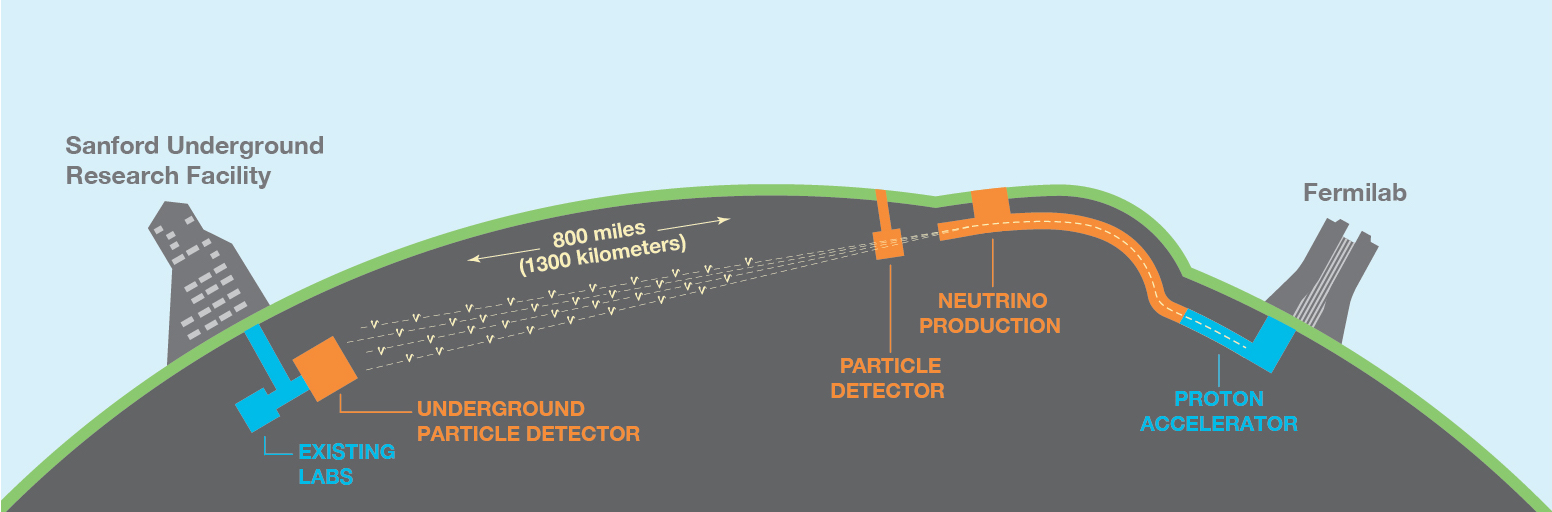
\includegraphics[width=\textwidth]{images/LBNE_Graphic_061615_2016.jpg}
\caption{Simple Draw up of DUNE FD taken from \citep{dune_cdr_2016_arxiv}}
\end{figure}

DUNE has three main science goals, all of which are geared towards pushing beyond the standard model:
\begin{itemize}
    \item Hadron Decay
    \item Neutrinos from Core-collapse supernovae
    \item Beamline neutrino interactions.
\end{itemize}

We will discuss the relevance of each of these items, and in \ref{chap:qpix} we will further discuss how the work presented here relates to each of these topics. 


Conventional horizontal drift detection for foreseeable DUNE modules are already considered possible for lengths up to 6.5m \citep{DUNE_Vertical:Paulucci_2022}.


\subsubsection{Hadron Decay}
\label{sect:intro_decay}

Second generation proton decay studies in the ICARUS experiment: \citep{ICARUS_2001}.

%% why do we care about hadron decay

\subsubsection{Supernova Studies}
\label{sect:intro_supernova}

%% why do we care about supernova neutrinos, what will they tell us?
The principal decay chain follows the pattern:
\begin{equation}
    \nu_{e} + ^{40}Ar \rightarrow e^- + ^{40}Kr^*
\end{equation}

%% text from the cdr 
% The neutrinos from a core-collapse supernova are emitted in a burst of a few tens of seconds
% duration, with about half the signal emitted in the first second. The neutrino energies are mostly
% 4The lifetime shown here is divided by the branching fraction for this decay mode, $\tau$ /B, and as such is a partial
% lifetime.
% Volume 1: The LBNF and DUNE Projects LBNF/DUNE Conceptual Design Report
% Chapter 2: DUNE Science 2–18
% in the range 5–50 MeV, and the luminosity is divided roughly equally between the three known
% neutrino flavors. Current experiments are sensitive primarily to electron antineutrinos ($\nu_e$), with
% detection through the inverse-beta decay process on free protons5
% , which dominates the interaction
%rate in water and liquid-scintillator detectors. Liquid argon has a unique sensitivity to the electronneutrino (νe) component of the flux, via the absorption interaction on 40Ar,

% This interaction can be tagged via the coincidence of the emitted electron and the accompanying
% photon cascade from the 40K∗ de-excitation. About 3000 events would be expected in a 40−kt
% fiducial mass liquid argon detector for a supernova at a distance of 10 kpc. In the neutrino channel
% the oscillation features are in general more pronounced, since the νe spectrum is always significantly
%different from the νµ (ντ ) spectrum in the initial core-collapse stages, to a larger degree than is
%the case for the corresponding ν¯e spectrum. Detection of a large neutrino signal in DUNE would
% help provide critical information on key astrophysical phenomena such as
%  the neutronization burst,
%  formation of a black hole,
%  shock wave effects,
%  shock instability oscillations, and
%  turbulence effects.
% In addition to yielding unprecedented information on the mechanics of the supernova explosion,
% the observation of a core-collapse supernova in DUNE will also probe particle physics, providing
% neutrino oscillation signatures (with sensitivity to mass hierarchy and “collective effects” due to
% neutrino-neutrino interactions), as well as tests for new physics such as Goldstone bosons (e.g.,
% Majorons), neutrino magnetic moments, new gauge bosons (“dark photons”), “unparticles” and
% extra-dimensional gauge bosons

%% what is the difference between NC and CC neutrino interactions.

\section{Even Further: Detectors in the Current Century}

Finally, in this last section we discuss recent development of various detector technologies.
There are many motivating pressures for new detectors to adopt pixelated designs. 
Below we discuss two contributing factors: the development of electronics and computing algorithms.

First, previously pixelated detectors have historically been more difficult because of the issues of cost and size regarding the number of readout channels.
This is being addressed, in part, by the advent of newer, cheaper, and larger Field-Programmable-Gate Arrays (FPGAs).
One method for reducing the electronic overhead required in pixelated detectors is to use digital multiplexing.
Cheap, high channel FPGAs directly solve this problem. 
Other electronics development, such as the Silicon-Photomultiplier, offer much cheaper alternatives for large pixel counters compared to their historical counter-parts. 

%% antihydrogen
\citep{Sadowski_2017}
Another driving factor is the the development of Machine Learning (ML) algorithms, particularly Convectional Neural Network (CNN \citep{Sadowski2017DeepLI}). 
Recent industry has driven the need for CNNs to be able to correctly identify and label 2-D images of various kinds, and thus championed much of progress in this field and spawned many kinds of CNN algorithms. 
%% cite sadowski here
Recently, it has been shown how these kinds of algorithms extend into High Energy Physics (HEP) for particle identification.
A major issue at the Intensity Frontier of physics is the sheer amount of data to store and process. 
These ML algorithms provied a developed tool to automate the analysis of huge amounts of data ($>> 1 TB$) and have been shown to be quite accurate ($>99\%$) at particle identification in LArTPCs.

%% LArPix / Argon Cube
\subsection{Current Pixelization Efforts in TPCs}

%% goeldi inspiration here from LArPix

Additional work has been performed in recent years which show that LArTPCs can also utilized a pixel-based readout \citep{larpix:Dwyer_2018}, \citep{Asaadi_2018}.



\subsection{SANDD}

Another Example of a pixelated detector is \citep{SUTANTO2021_sandd_165409}.


\subsection{The Single Volume Scatter Camera}

This work is presented in greater detail in (Appendicies-\ref{chap:OS1}/\ref{chap:OS2}) and represents a substantial amount of my own individual contribution. 
I am the 2nd author on the the paper described in Appendix-\ref{chap:OS1} and the corresponding author of Appendix-\ref{chap:OS2}, where I also collected and analyzed all presented data therein.

\subsection{Future Detectors}

The end of the Standard Model era is inevitable.
SM simply fails to account for physics with all major frontiers for physicists to accept its completeness; we know there is much and more to learn about nature.

The 20th century saw unprecented progress in its sophistication of its detectors from ray tubes, to spark chambers, to proportional counters, and to huge (>20 km) particle accelerators.
This century shows no signs holding any less promise than its predecessor.
Continued development in electronics, computing, and analysis methods will lead to more and newer frontiers of physics.

The work presented in this introduction aims to not only encapsulate the massive progress particle physics has made since the electron's discovery, but also to server as a reminder of how extraordinally surprising nature is.
At every turn and at every point where physicists think they've arrived at the end (or at an impossible roadblock) there always remains more to discover.
If we have learned anything, we have learned to knock and the door shall be opened.


%% chapter 2, the QPix Design concept
\chapter{A Novel Readout Technique for TPCs: Q-Pix}
\label{chap:qpix}
In this chapter we introduce a novel readout technology at the pixel level for LArTPCs. 
The basic readout circuit was first introduced by \citep{qpix:nygren:mei}.

Pixel based readouts offer several advantages over the traditional wire readout \citep{lartpc_recon_problems_joshi_2015}.
The key improvement offered is true 3-D image reconstruction. 
This allows for sharper vertex reconstruction, thereby improving the overall resolution of DUNE and decreasing the required time for a NP measurement.
Other advantages rely on data analysis and data storage. 
A pixel based readout automatically records 2 of the three spatial dimensions, and thereby provides for simpler analysis.
Additionally, the pixelated readout method presented here cuts the total required data storage and data acquisition rate (without loss to precision) by several orders of magnitude.

However, the advantages also come with the cost of increased design complexity as the number of readout channels increases by more than three orders of magnitude. 
The traditional wire based readout within a DUNE module will include hundreds to thousands of channels, whereas a full DUNE module with a pixel-based readout will have 10's of millions of channels.
This number of required channels to be stably readout during DUNE's expected lifetime ($> 10$ years), where the electronics continually operate at liquid argon temperatures is likely the largest hurtle for a pixel-based design.
The aim of this dissertation is to address the channel-size problem.

\section{Q-Pix: The Circuit Level Design}

Concept of this combined ASIC and reducing the number of channels relies on digital multiplexing.

This differs from other concepts such as Genetic Multiplexing (\citep{PROCUREUR2013888_genetic_multiplexing}) and using only regions of interest (ROI).

\begin{figure}[]
\centering
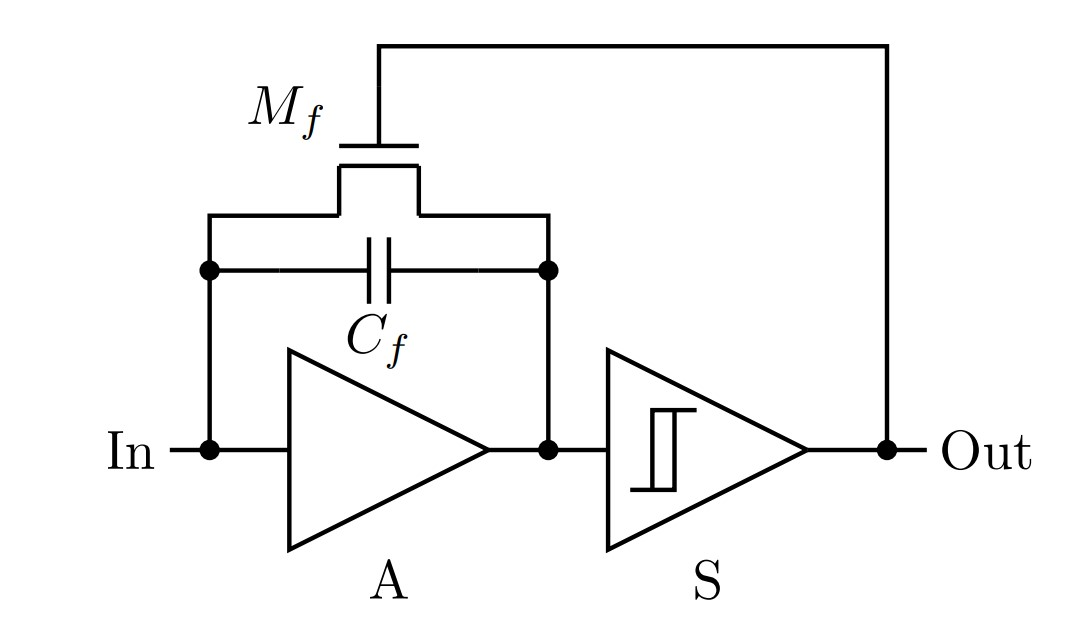
\includegraphics[width=\textwidth]{images/qpix_circuit.jpg}
\caption{Image of Basic Q-Pix Readout circuit. Currently this is being designed within a custom analog ASIC. Image is taken from \citep{qpix:nygren:mei}.}
\end{figure}


\begin{figure}[]
\centering
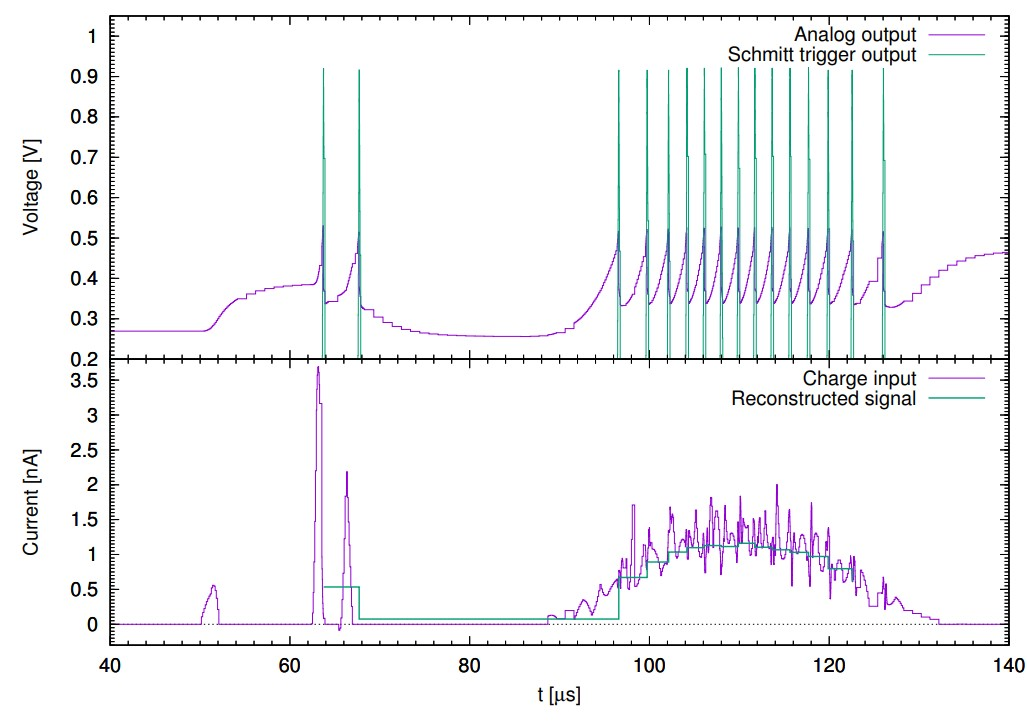
\includegraphics[width=\textwidth]{images/qpix_rtd_reconstruction_example.jpg}
\caption{Example reconstruction of the reset time difference (RTD) based on the Q-Pix readout design. Image is taken from \citep{qpix:nygren:mei}.}
\end{figure}

\begin{figure}[]
\centering
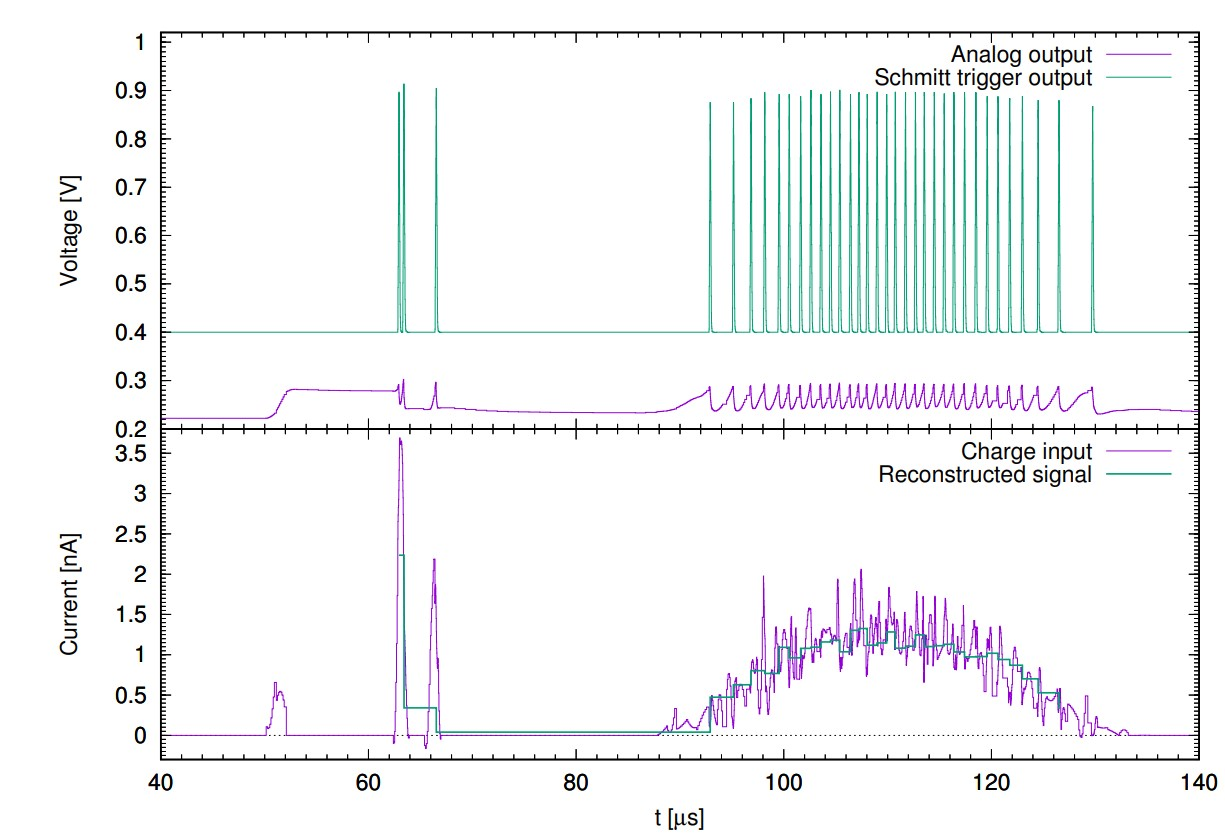
\includegraphics[width=\textwidth]{images/qpix_rtd_reconstruction_example_03fc.jpg}
\caption{Example reconstruction of the reset time difference (RTD) based on the Q-Pix readout design. delta-Q was chosen to be $0.3 fC$. Image is taken from \citep{qpix:nygren:mei}.}
\end{figure}

\section{System Requirements}

\section{How Q-Pix fits into a DUNE APA}

DUNE Anode Plane Assemblies (APA) designs are based on \citep{DUNE-FD_TDRv4:Abi_2020}.

%% example image of DUNE-APA from DUNE-FD TDR.
\begin{figure}[]
\centering
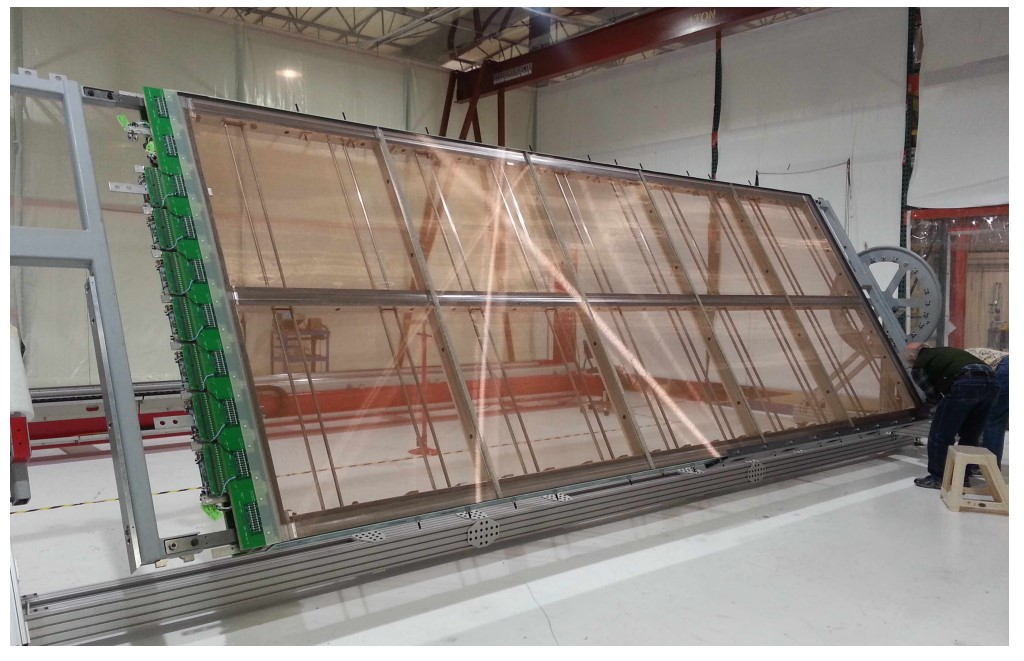
\includegraphics[width=\textwidth]{images/dune_fd_tdr_apa_image.jpg}
\caption{A simple caption \citep{DUNE-FD_TDRv4:Abi_2020}}
\end{figure}


%% chapter 3 - cap everything off with extended simulation studies based on results
\chapter{The First Prototype: First Resets and Leakage Measurements}
\label{chap:saq}
In this chapter, we present the first implementation of the Q-Pix-based design using off-the-shelf electronics.

This section describes the first prototype based on the Q-Pix readout: The Simplified Analog Q-Pix (SAQ).
First we discuss the design goals of the prototype and highlight the basic building blocks of any Q-Pix based prototype.
Next, We describe the prototype status as well as lessons learned in characterizing noise and performing calibrations.

In the final part of this section we describe the future goals of this prototype, including the addition of GEMs to the experimental setup.
The full results of the planned diffusion measurements are beyond the scope of this work, but we provide the initial details here because these measurements will ultimately provide the complete description of the prototype.

\section{Simplified Analog Q-Pix: System Design}

The SAQ prototype is designed as a first physical proof-of-concept for a Q-Pix readout.
The intended use

\section{The SAQ Protoype Design}

\begin{figure}[]
\centering
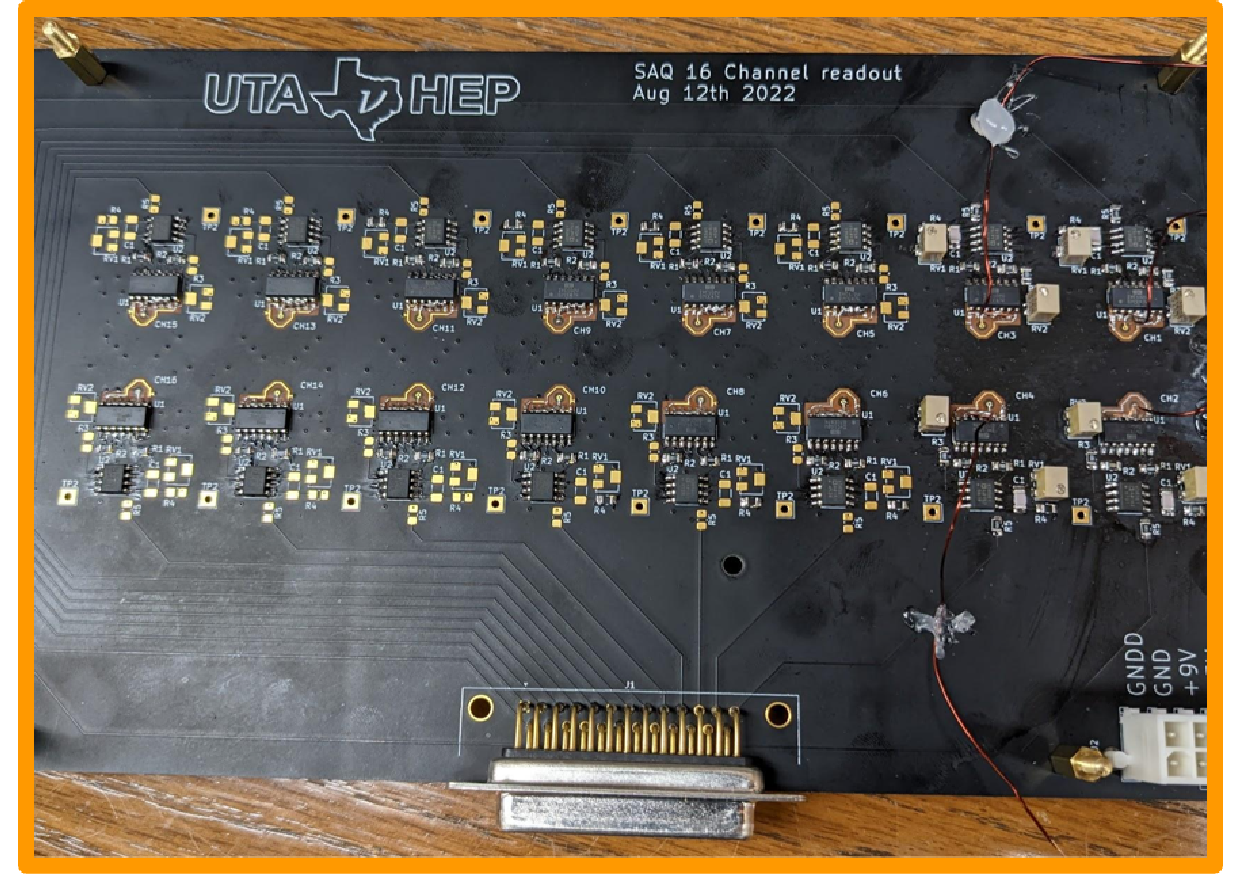
\includegraphics[width=\textwidth]{images/SAQ_16_ivc_readout_board.pdf}
\caption{The SAQ Setup model based on~\ref{}.}
\end{figure}~\label{fig:saq_readout_board}

%%
\begin{figure}[]
\centering
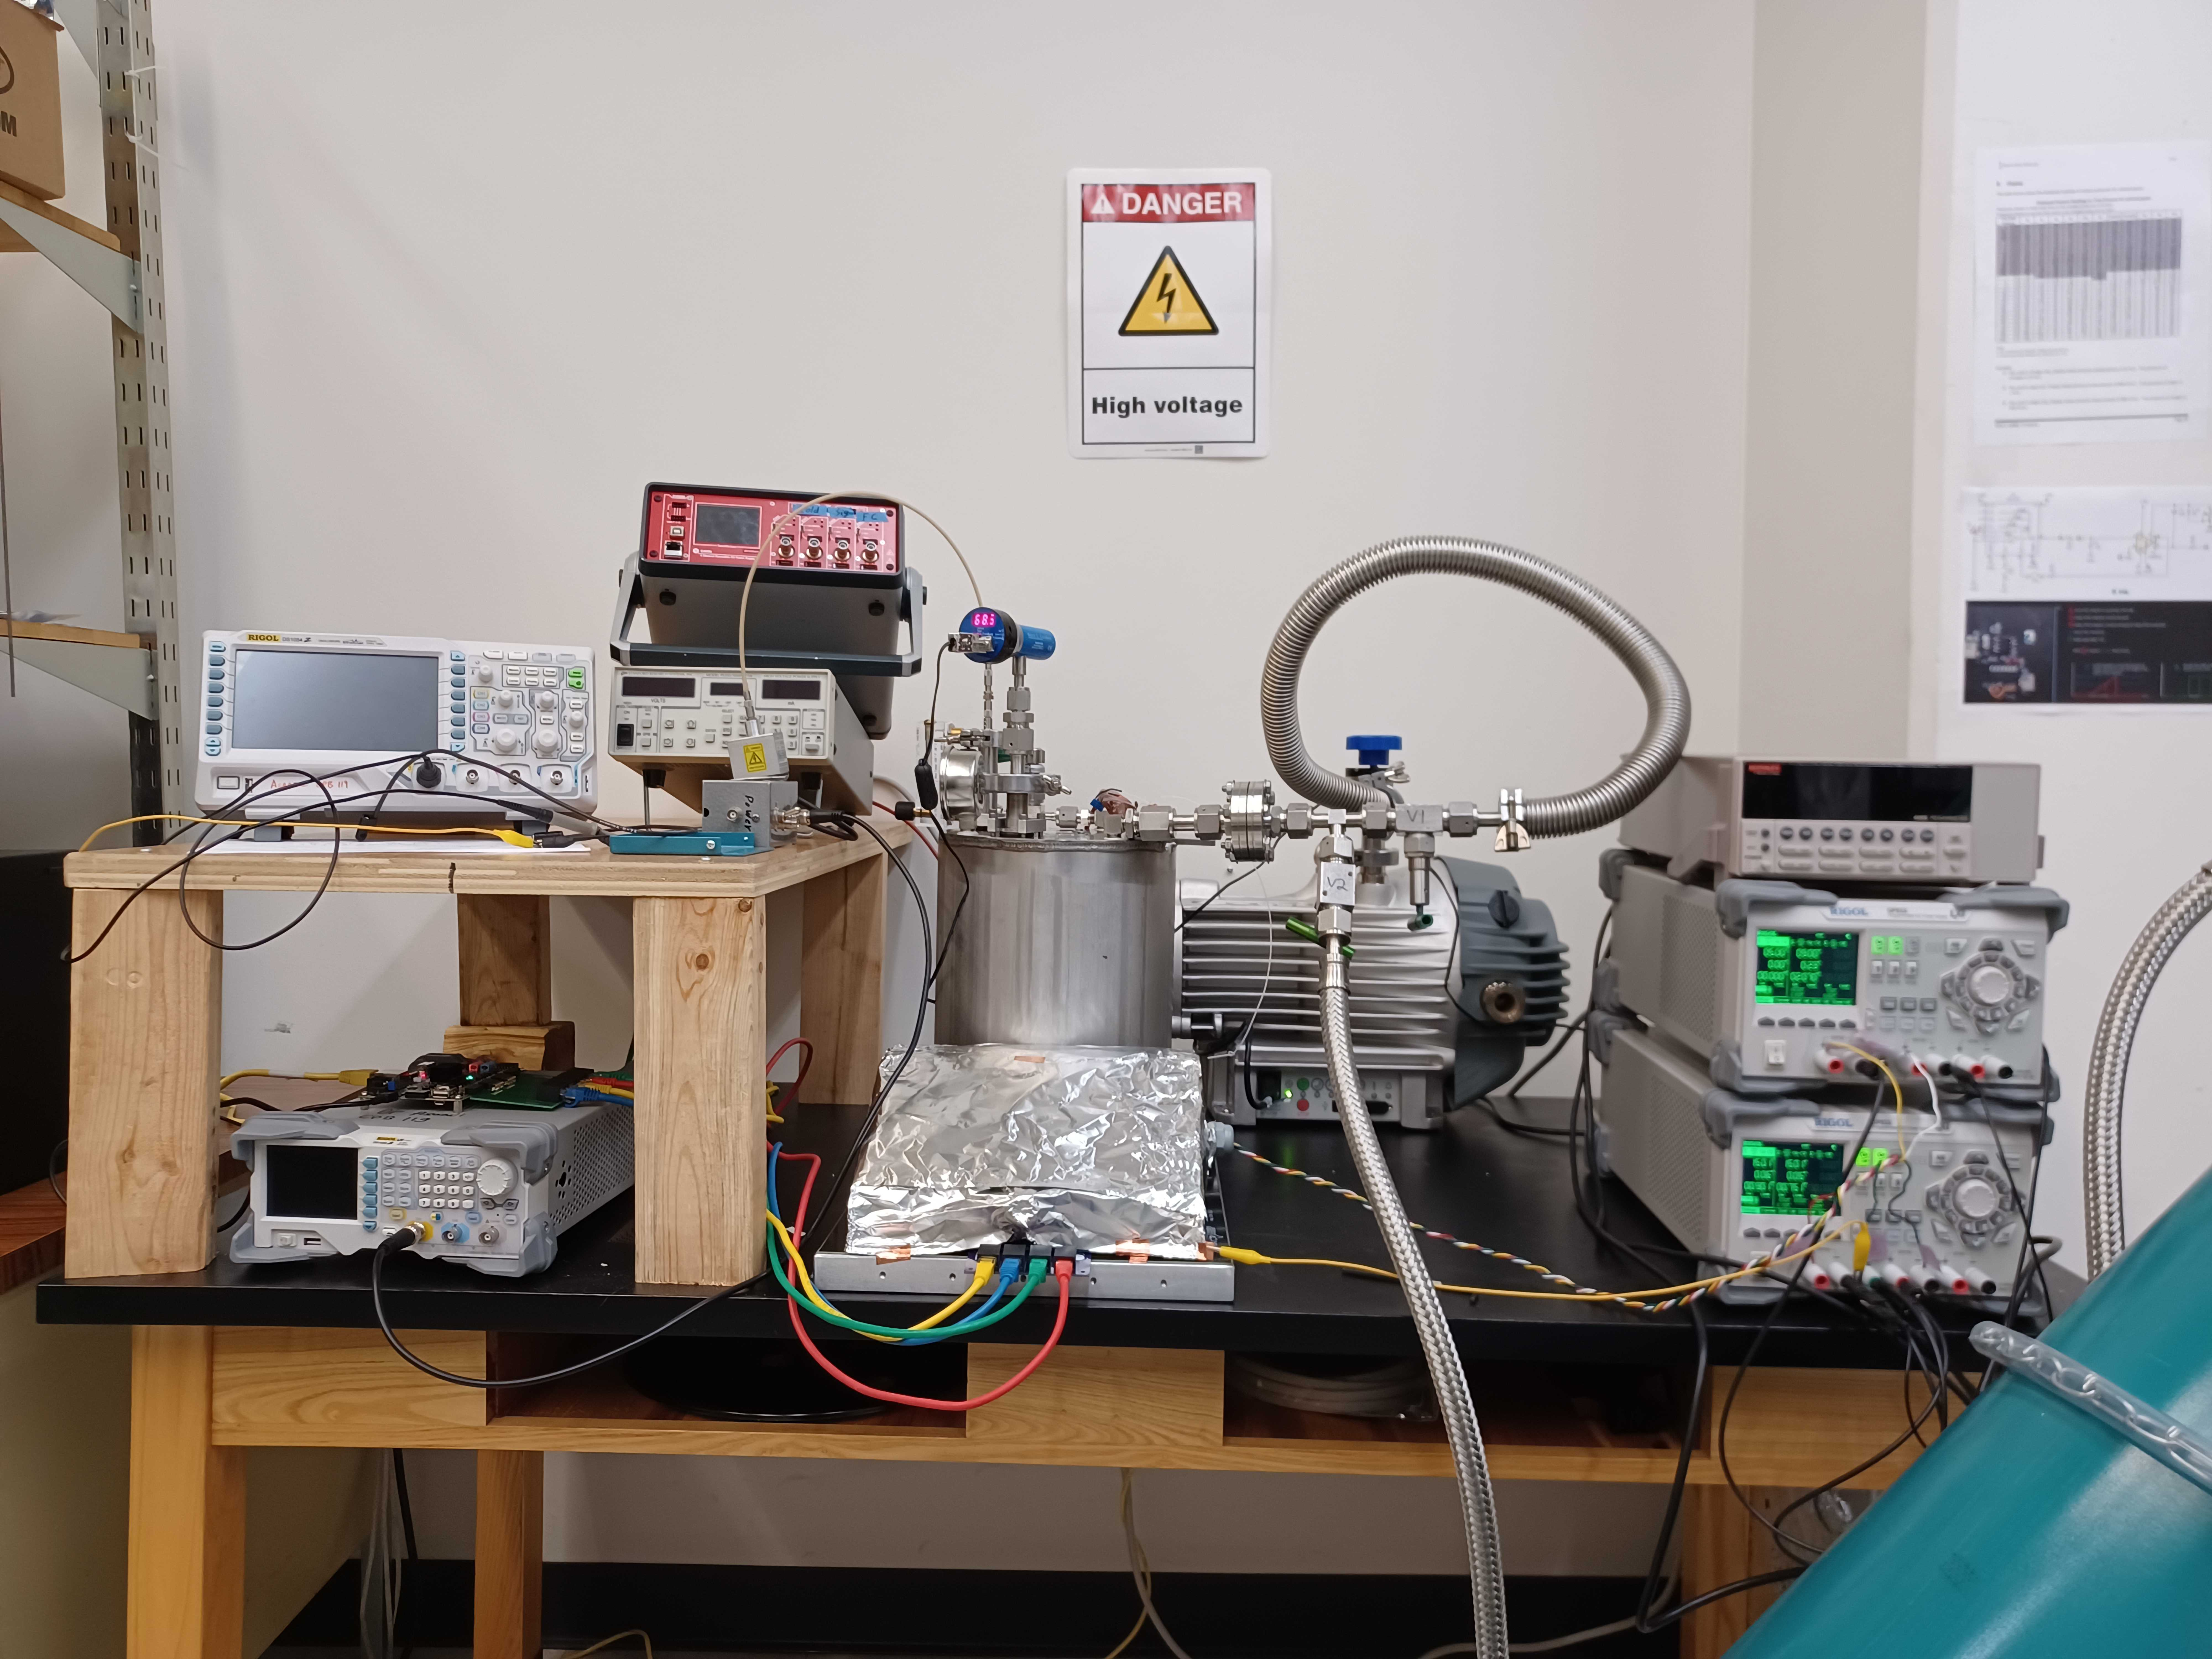
\includegraphics[width=\textwidth]{images/SAQ_physical_setup.jpg}
\caption{The SAQ Setup model based on~\ref{fig:saq_setup_physical}.}
\end{figure}~\label{fig:saq_setup_flatten}

\begin{figure}[]
\centering
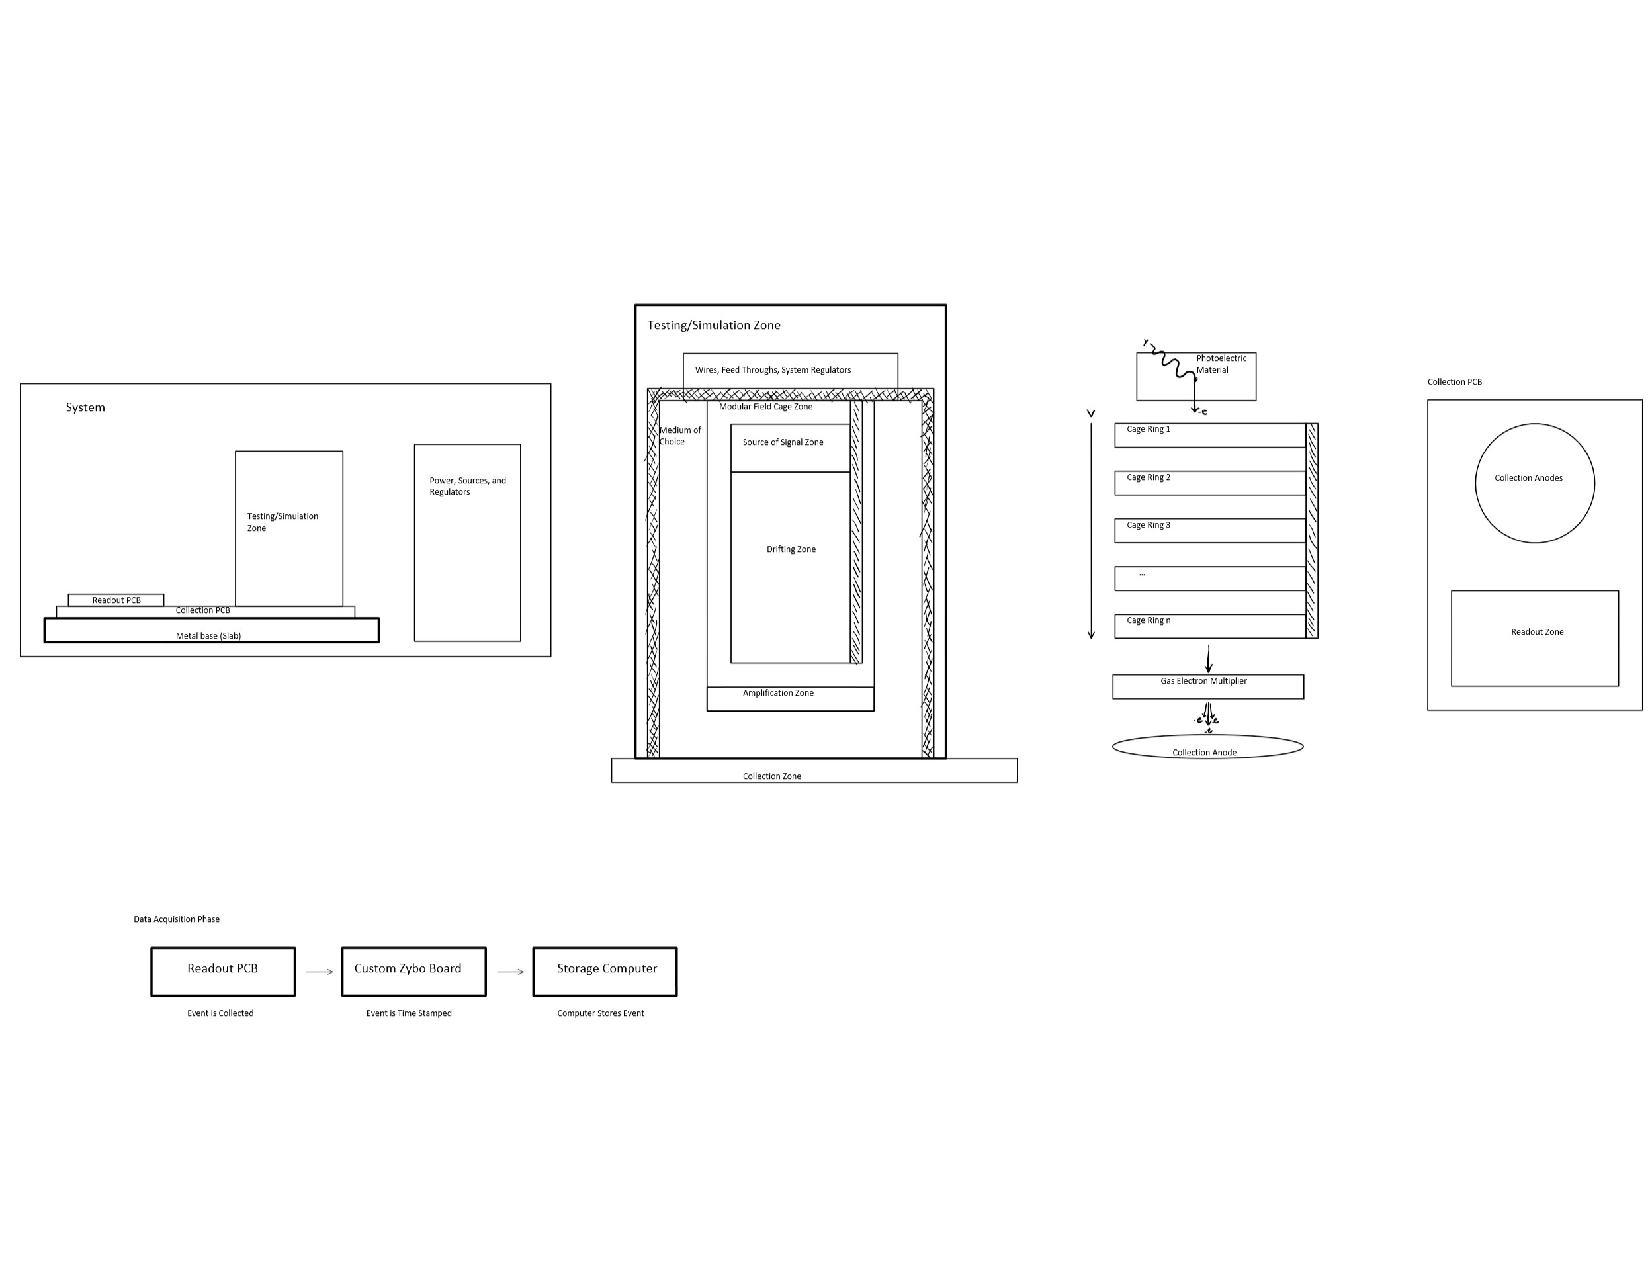
\includegraphics[width=\textwidth]{images/SAQ_setup_diagram.pdf}
\caption{The SAQ Setup model based on~\ref{fig:saq_setup_diagram}.}
\end{figure}~\label{fig:saq_setup_flatten}

\subsection{The TPC Design}
%% closeup image of the TPC here

\subsection{The Integrator Circuit}



\begin{figure}[]
\centering
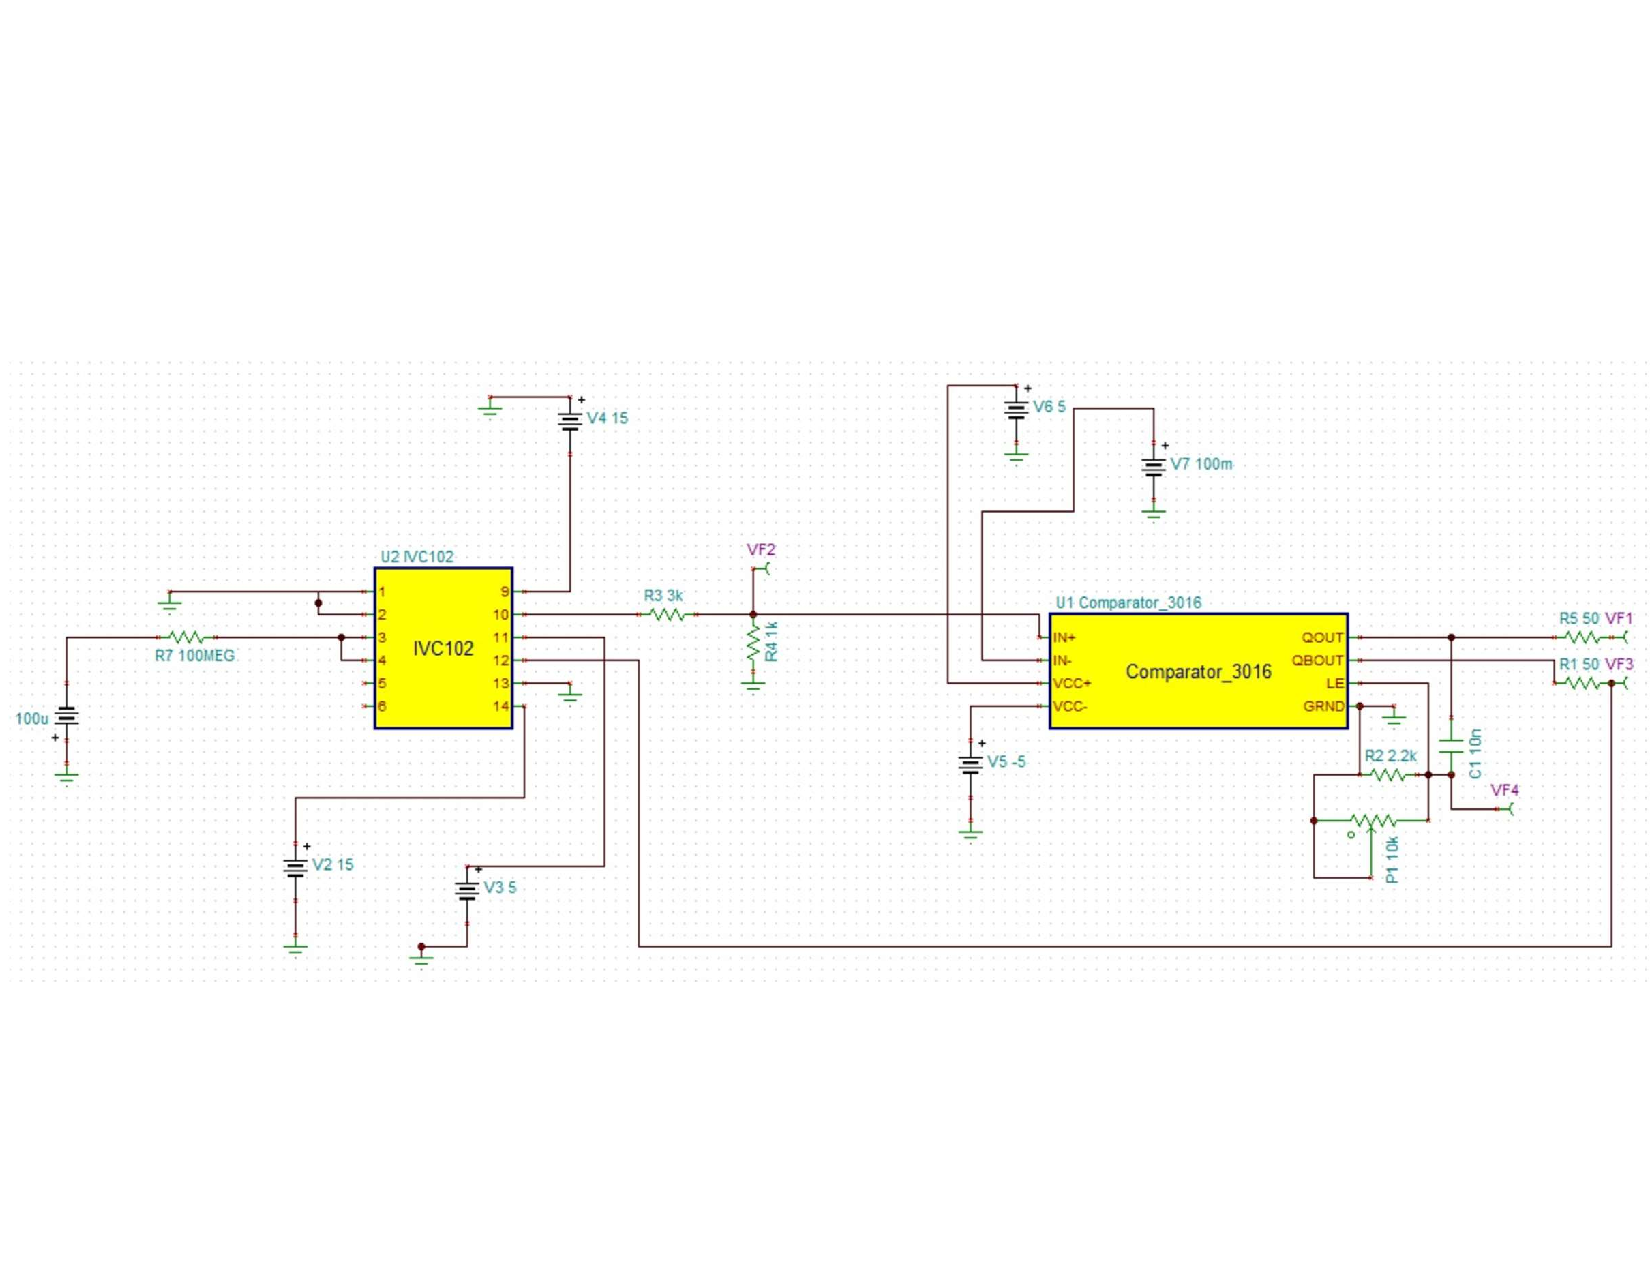
\includegraphics[width=\textwidth]{images/SAQ_spice_circuit.pdf}
\caption{The SAQ circuit in a Spice Simulation. The IVC~\citep{ivc_datasheet} chip chosen as the off-the-shelf integrator for this experiment. The main selection choice for this part is due to its low input bias current $\ll 750~\unit{fA}$.}
\end{figure}~\label{fig:saq_circuit_spice}


\subsection{The SAQ Data Acquisition}

All resets are recorded via a Zybo-Z7-20 Digilent FPGA prototype board, which uses an Artix Zynq based archticture.
The reference manual for the Zybo Z7 board used in SAQ can be found at \citep{zybo_zy_reference}.

\begin{figure}[]
\centering
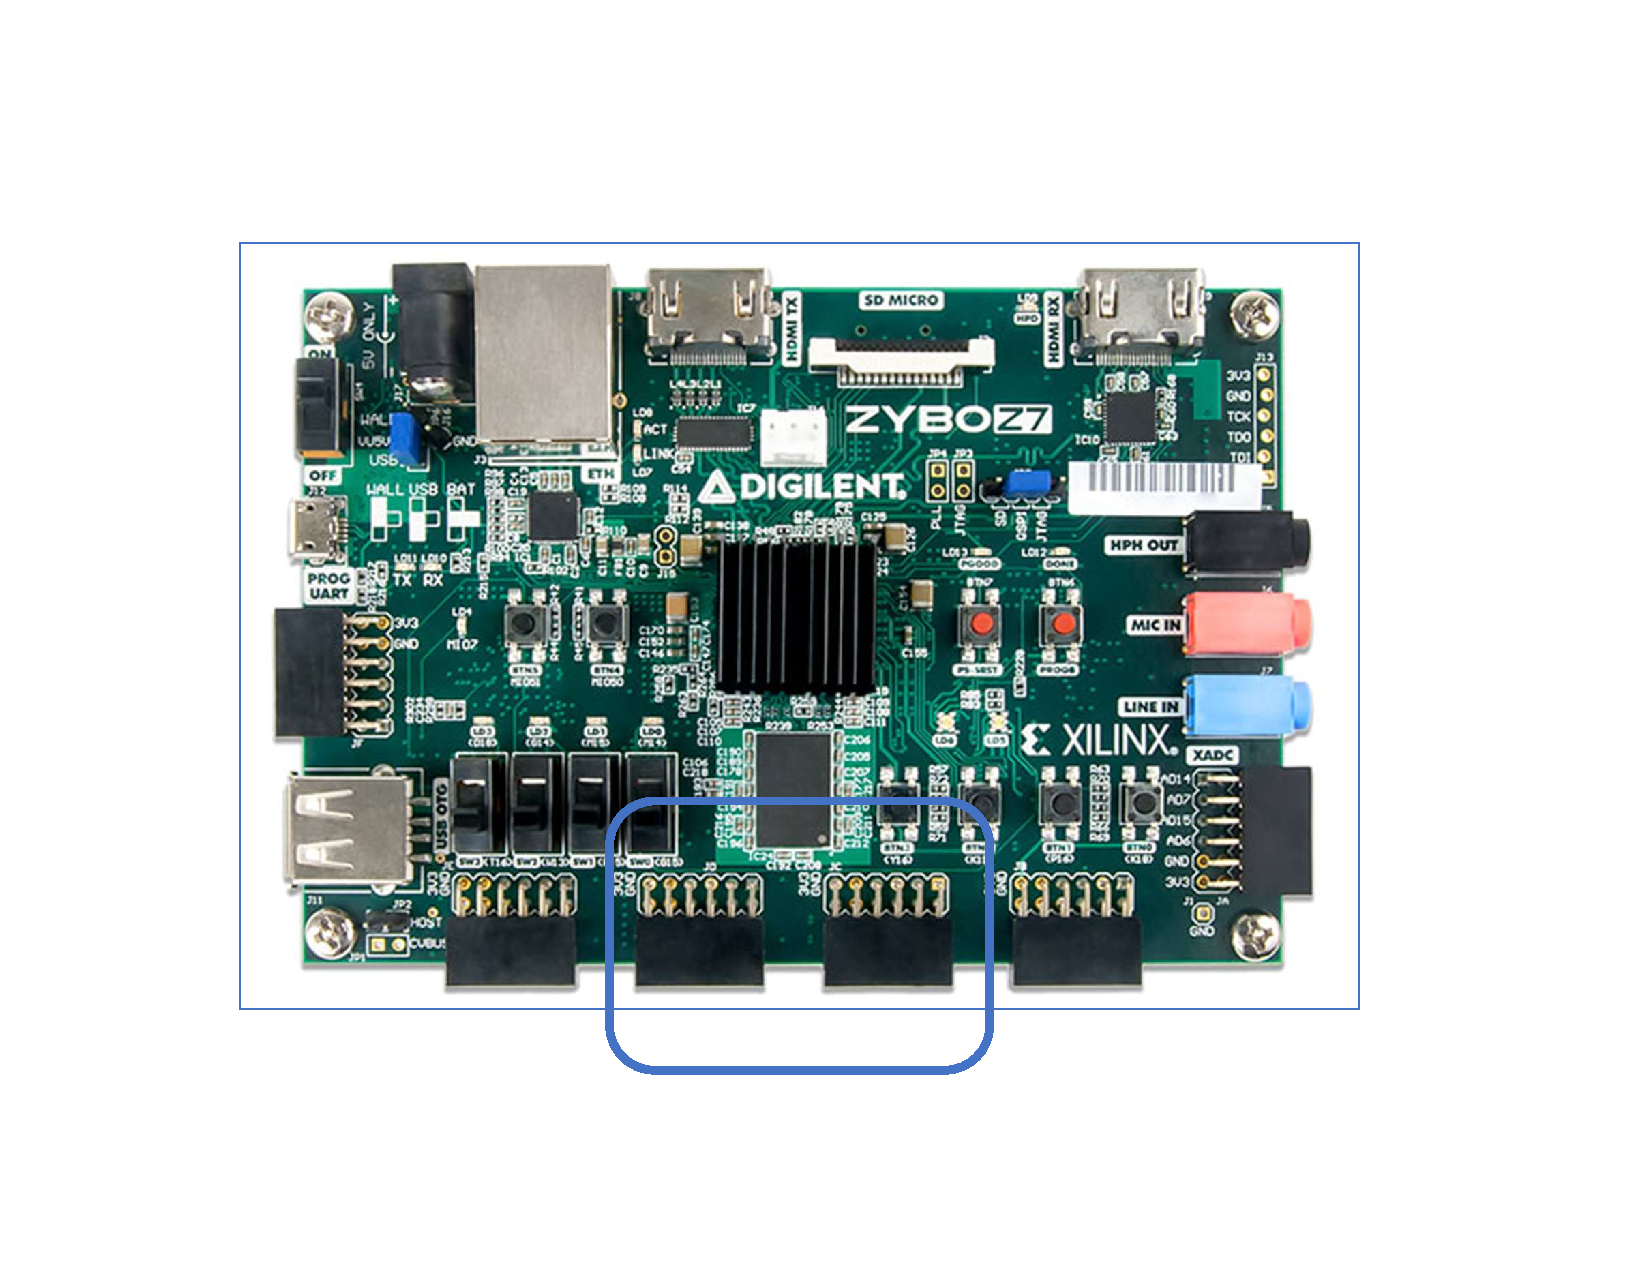
\includegraphics[width=\textwidth]{images/SAQ_zybo_daq.pdf}
\caption{An image of the data acquisition board from Digilent, Zybo Z7-20. This board was chosen for its multiple configurable input chanels, as well as the Zynq-based archiecture of the onboard FPGA. Additionally, the use of the ethernet provides $1~\unit{GB}$ transfer speeds, which is more than sufficient for the application.}
\end{figure}~\label{fig:saq_zybo}

\begin{figure}[]
\centering
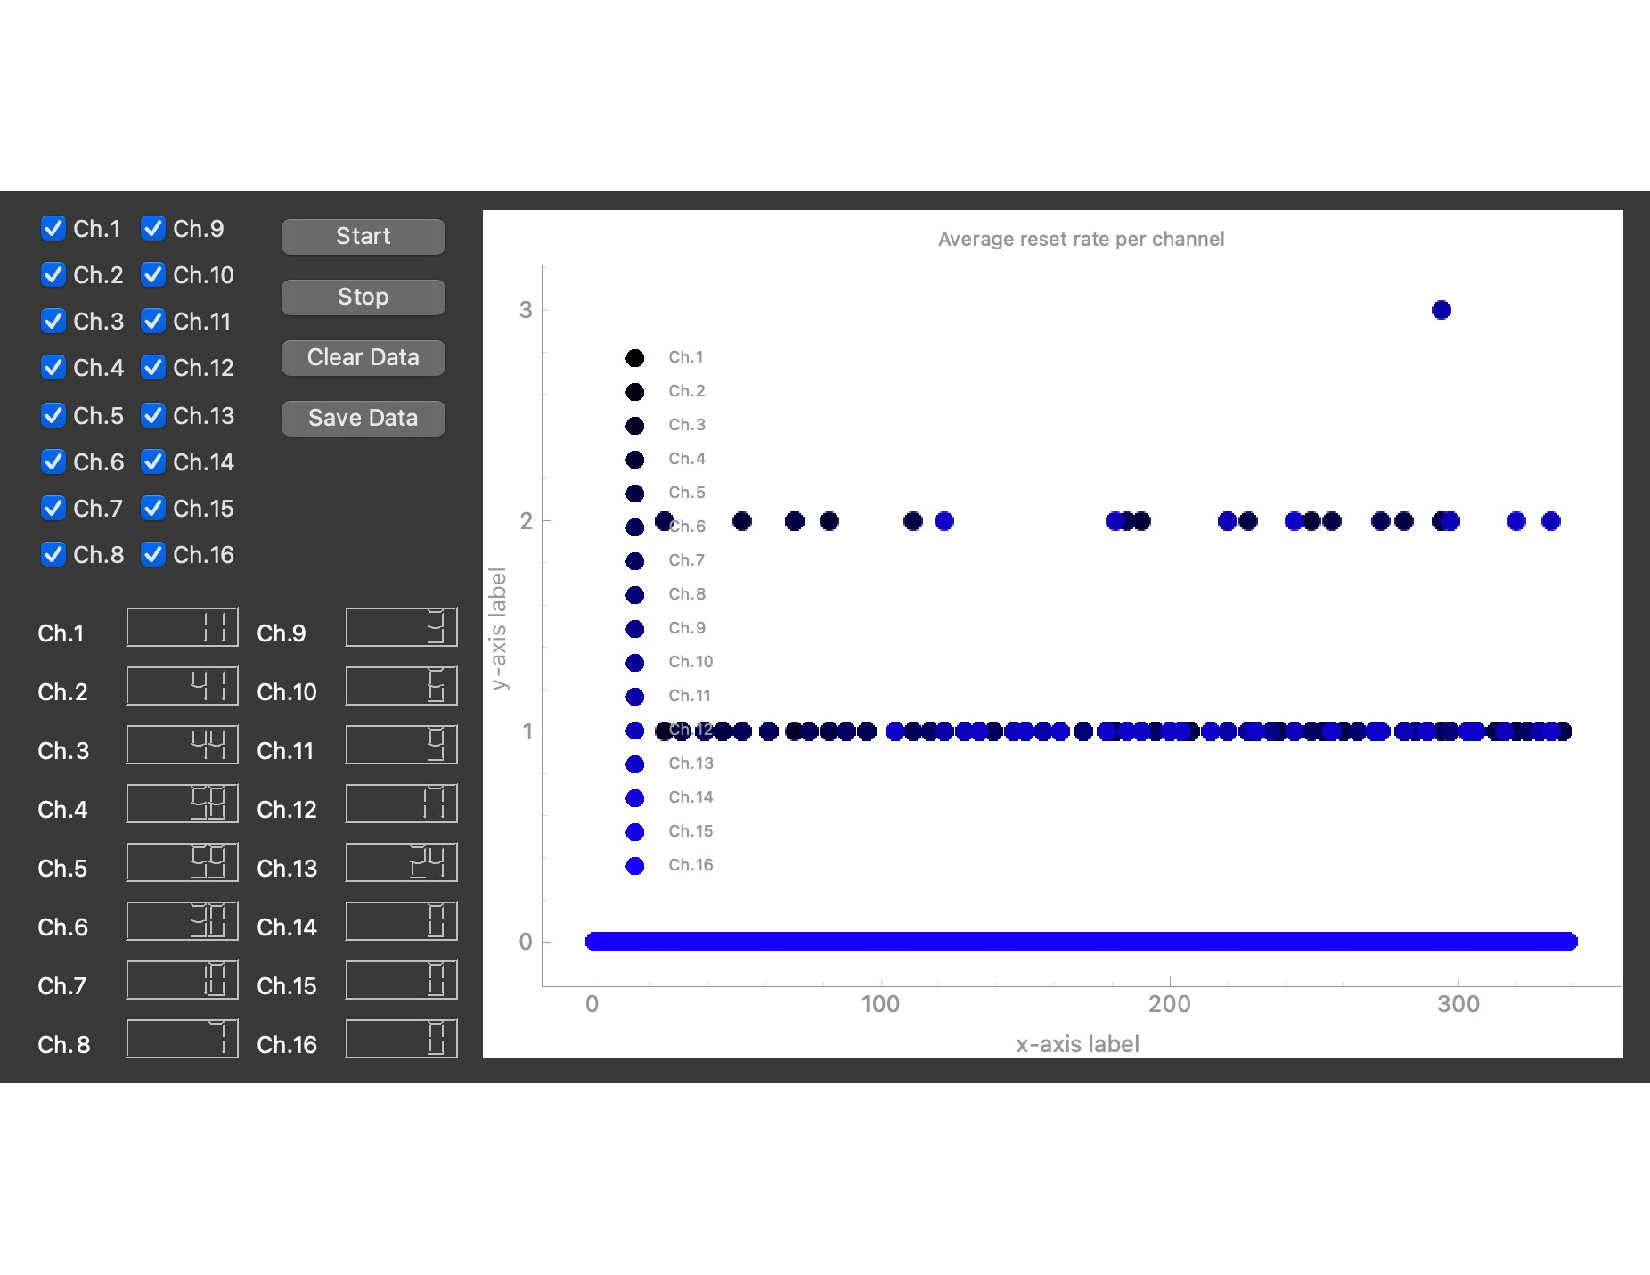
\includegraphics[width=\textwidth]{images/SAQ_gui_resets.pdf}
\caption{The SAQ GUI with real time plotting of incoming resets to the Zybo board.}
\end{figure}~\label{fig:saq_gui}


\section{Noise Measurements}

The Q-Pix readout is dependent on the integrator, which provides the basic datum of the reset time.
Therefore, a dominant source of noise are electrons which accumulate on the integrator which are not signal electrons.
There are two possible sources for these noise electrons: excess electrons produced from the target volume or leakage current due to transistor effects from the integrator circuit.
In this section we focus on the noise electrons due to the leakage current.

\subsection{Integrating towards background Current}

Leakage current arrises due to non-idyllic behavior of the integrator operational amplifier, where the voltage across the two input terminals is nonzero.
Measurements of this leakage current then are performed by measuring voltage difference across the terminals as well as directly using a pico-ammeter.

\subsection{Integrating towards background Current}

%% describe setup / filling of TPC here
The second source of noise electrons are produced from the target volume.
The target volume is an ultra pure Argon Gas at TODO militorr.
% 14 psi with argon (0.069 bar)
% And ~3mtorr of vacuum before that
In this case the excess electrons come from the nominal decay of Ar-39, which provide excess electrons from the natural $\beta$ decay, at a rate of $\approx 1~\unit{Bq}{Kg^{-1}}$

\subsection{Digital Noise Sources and Clock Stability}


\section{Xenon Gas Lamp Measurements}

\begin{figure}[]
\centering
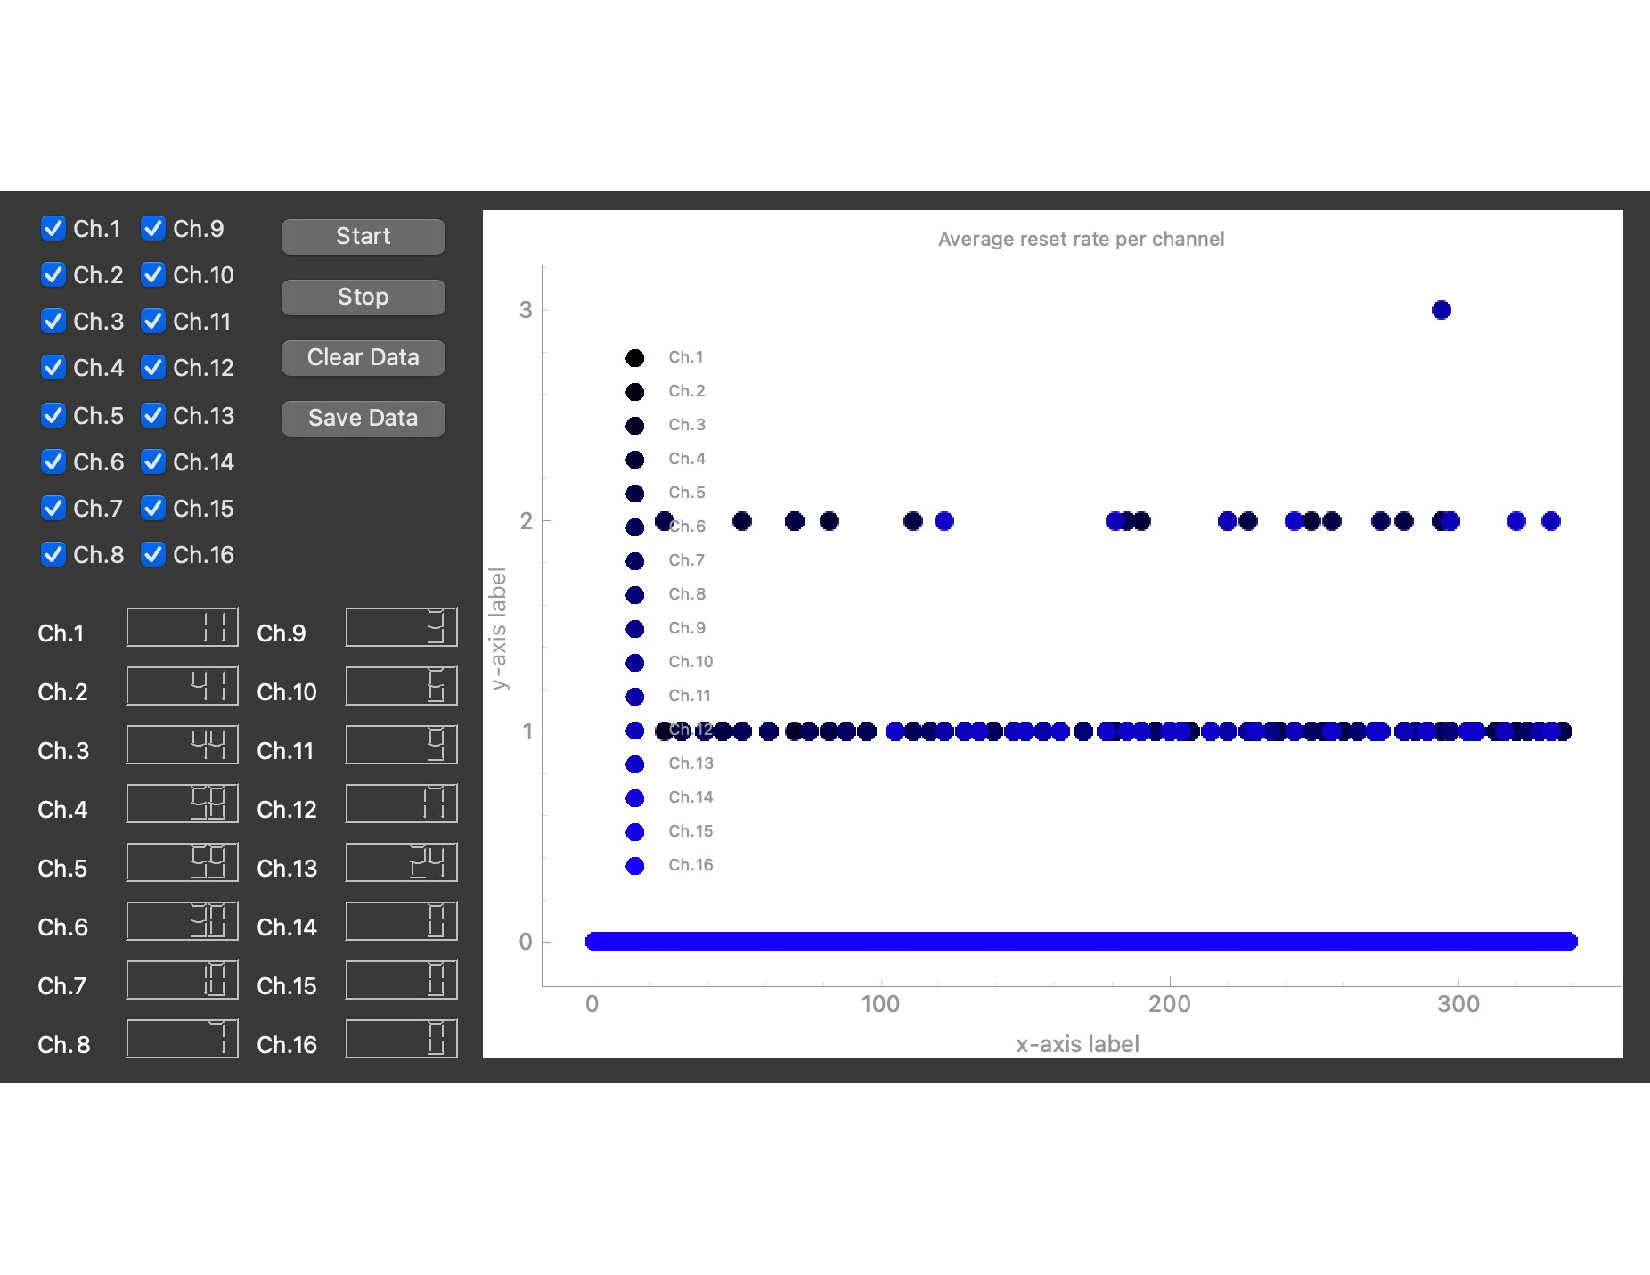
\includegraphics[width=\textwidth]{images/SAQ_gui_resets.pdf}
\caption{Drift Current Measurements to go here.}
\end{figure}~\label{fig:saq_drift_gui}

\section{Results and Discussion}

\begin{figure}[]
\centering
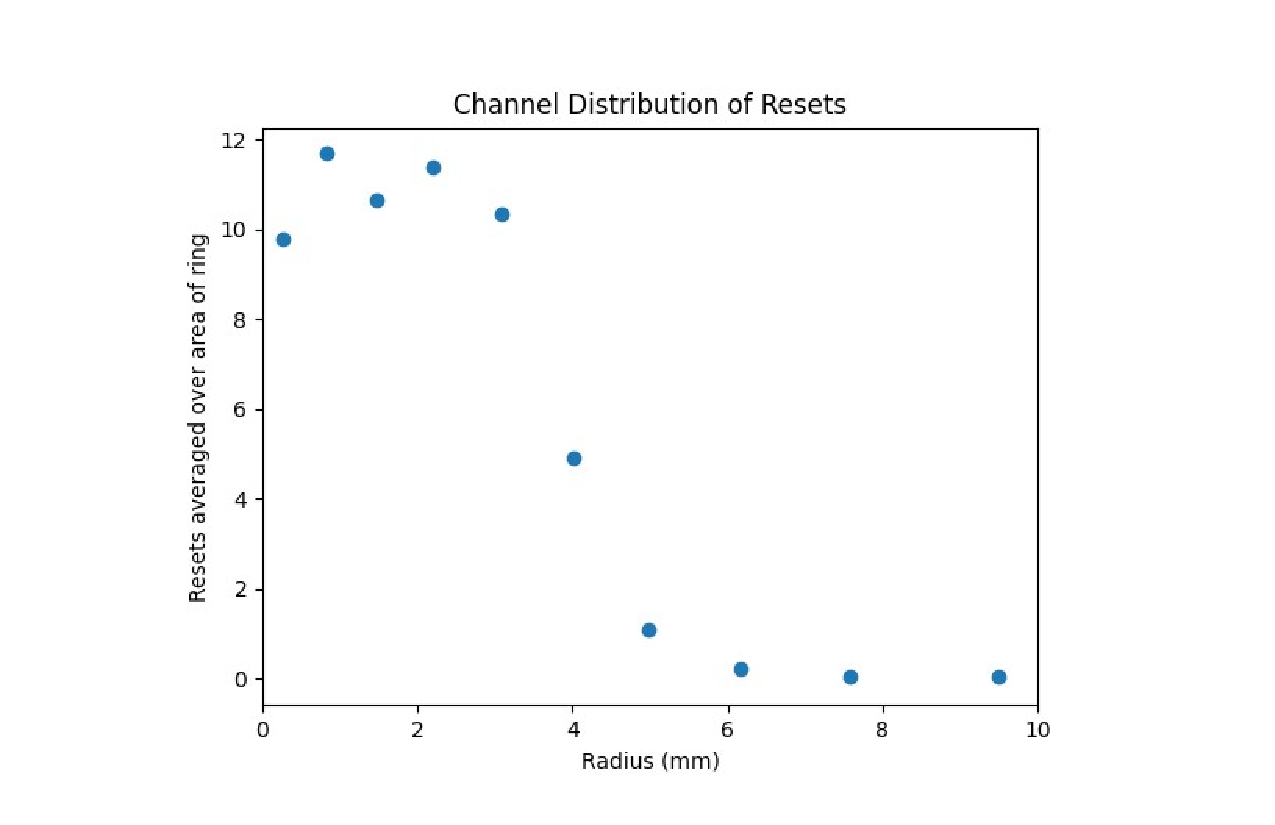
\includegraphics[width=\textwidth]{images/SAQ_first_diffusion_measurement.pdf}
\caption{First diffusion measurement in P-10 gas performed at Wellesy University.}
\end{figure}~\label{fig:saq_first_diffusion_measurement}

\subsection{Current Status and Planned Measurements}

Measurements of Transverse and Longitudinal diffusion of electrons within electric fields of strength 500 V/cm have been performed before \citep{lar_diffusion_measurement_LI2016160}.


%% chapter 4
\chapter{Digital Back-end Viability Studies}
\label{chap:qdb}
In this chapter we describe the overall structure of the digital back-end of the Q-Pix design as well as results from prototype board tests.
As described in previous chapters, the digital back-end of the Q-Pix readout is composed of an array of ASICs (FPGAs, here), which we refer to here to as digital nodes.
Each digital node in the prototype array is implemented as a lattice ice40UP5k FPGA.

This chapter is divided into two parts.
The first part we give a detailed description of the requirements of a successful deployment digital-system in a Q-Pix based detector at DUNE APA scales.
The motivation is to describe how the digital backend of Q-Pix based readout would eventually scale into a DUNE-FD LArTPC 10 kT module.

The second part of this chapter is dedicated to the first evaluation boards developed and tested which implement the digital nodes in Lattice iCE40UP FGPAs~\citep{lattice_ice40up_datasheet}.
The second part also outlines the design of the PCB on which these FPGAs are implemented, as well as results, which are motivated from the first part of this chapter.

The Lattice Semiconductor FPGAs \citep{lattice_ice40up_datasheet} were selected because of the small form factor, pin out, availability, as well as low power consumption.
There are planned tests for future, but not presented here, to indicate its viability of over-the-counter FPGAs in LArTPc.
If such cheap and available FPGAs were shown to be reliable use in a LArTPC environment, that could influence future detector development and the selection of the digital chip for the Q-Pix readout.

All results presented in this chapter are my own individual work.

\section{Digital Design Overview}

The digital system of the Q-Pix readout begins when the first digital data are recorded.
This occurs during the collection of a recorded timestamp in response to the logic reset pulse sent from the integrating analog front-end.
This record happens in response to output reset-pulse sent from any one, or more, of the pixels.
Then, the timestamp record is the value of a local 32-bit counter at the time the node receives the reset pulse.
When a reset occurs the data recorded are the reset values of each pixel, and the only data required for a full analysis of all reconstruction with a LArTPC are:

\begin{figure}[]
\centering
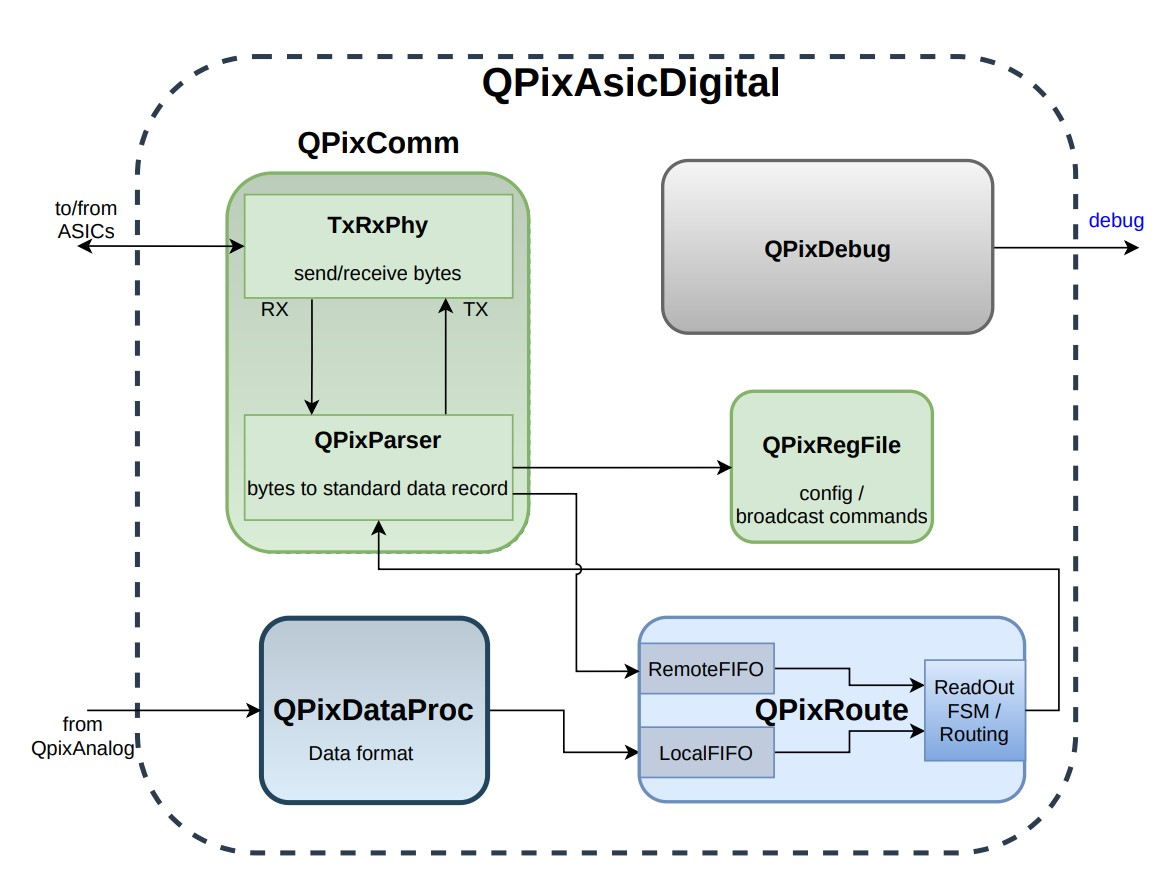
\includegraphics[width=\textwidth]{images/digital_node_overview.jpg}
\caption{Diagram of the Digital node.
  The controlling sections of the logic for the digital node are QpixComm, QPixDataProc, QPixRoute, and QPixRegFile.
  The Comm layer is responsible for routing packets between the physical layer and handles the parsing of incoming data packets.
  The DataProc layer is responsible for recording timestamp data during a reset from the analog front-end.
  The RegFile contains configuration information, such as routing.
  QPixRoute determines the controlling state machine that, based on register configurations, determines what packets are sent to which neighboring nodes.}
\end{figure}~\label{fig:qpa_diagram}

Each of these remote ASICs are running on free-running independent clocks, with an expected frequency of $\approx$ 30 MHz.

\subsection{Communications}

The QpixComm module controls incoming and outgoing packet logic.

The logic responsible for indentifying how an incoming packet is handled is defined in QPixParser.
When a valid 64 bit packet has been received, a valid signal is thrown high.
The packet is handled based on the bits within the header of this packet.
How the packet is handled is determined the by the packet header~\ref{bit_reservation}.

Packets are only comprehensable for types if the same region of the 64 bits are ubiqutous.
For this purpose all packets use or reserve the same 20 bits, with four bits reserved for the packet type:

\begin{itemize}
    \item Unused, 60--63
    \item Header, 56--59
    \item X Location, 36--39
    \item Y Location, 32--35
\end{itemize}~\label{bit_reservation}

If the packet originated from the aggregator node then this packet is treated as a broadcast.
Broadcast commands record unique numbers associated with this request and are also sent to all connected neighbornoods except from the direction that the broadcast is received.
A unique broadcast number is used to avoid registering the same request.

If the packet was not from an aggregator node, then this packet is treated as remote data from a neighbor node.
All data transfers of any kind are treated so that all communication happens between individual nodes and an aggregator node.
Therefore, any packet that originates on a node that isn't the aggregator node will be sent to the aggregator node.
The direction of that this packet is sent is deteremined by a configuration register.

\subsection{The Structure of a Data Word}

Each digital node responds to a successful transmission of a 64-bit packet.
We choose that each packet, regardless of type, be 64-bits to reduce the overall packet checking complexity on each node.
The type of the packet then is selected by the word type, which is reserved for a static 4 bits within each 64-bit word.
This allows for a total amount of 16 unique packets each of which may be handled differently.

A successful transmission of a data word is indicated by the protocol when the correct number of bits have been read~(see Section~\ref{sect:endeavor}).
When a correct packet is filled a single flag is raised to indicate that the word is valid, and then the appropriate logic parses the header bits of the packet and determines how the packet should be handled.

There are two main types of packets that a digital node would receive, a register request or a data word from another node.
In the first case, the register request indicates that this packet originated from the aggregator node and may either to a specific node or a broadcast to the entire array.
Whether or not the register request is a broadcast is checked against another bit, and the packet is handled accordingly.
If the packet is a broadcast, the receiving node records an identification number associated with the broadcast, which it uses to ignore additional packets it may receive that correspond to the same broadcast.

The second kind of packet the digital node may receieve is a data type word.
In the case of data words, there are also two main types: a word which contains the 32 bit timestamp or an event end word.
The 32 bit timestamp data word are the words which must eventually make it to disk for analysis.
The data words must also encode the row and column position of the original nodes.

\subsection{Configuration}

The configuration of the digital node is handled through local registers.
These registers are described within QpixRegFile module, shown in Figure.~\ref{fig:qpa_diagram}.
These registers include the ability to control routing of data packets, reset, enable, and channel masking.
The Table~\ref{tab:registers} describes the implemented register addresses and their functions:

\begin{table}
\begin{center}
\begin{tabular}{||c c c||}
 \hline
 Address & Name & Function \\ [0.5ex]
 \hline\hline
  0x01 & Command & Used to broadcast type or trigger \\
 \hline
  0x03 & Routing & Allows selection between manual or dynamic routing. \\
 \hline
  0x04 & Channel Mask & Selection of mask prevents triggers from masked channels. \\
 \hline
  0x05 & Position & Allows configuration of X and Y coordinates of node. \\
 \hline
  0x06 & Disable & Selection of which neighboard node inputs are ignored. \\
 \hline
  0x08 & Local Disable & Selection of which input and out neighboard nodes can be ignored. \\
 \hline
\end{tabular}
\caption{The address values are not sequential because some registers have become deprecated through development.}
\end{center}
\end{table}
~\label{table:node_registers}

The composition of any register word is shown in Table~\ref{tab:packet_register}.
\begin{table}
\begin{center}
\begin{tabular}{|| p{30mm} | p{30mm} | p{90mm} ||}
 \hline
 Bit Location & Name & Function \\ [0.5ex]
 \hline\hline
  0--15 & Data & Excess bits  \\
 \hline
  16--31 & Address & Excess bits  \\
 \hline
  40--43 & Y Position Transfers & Next Y position in tile. \\
 \hline
  44--47 & X Position Transfers & Next X position in tile. \\
 \hline
  48 & Source Flag & Single Bit flag to indicate whether ot not packet originated from aggregator. \\
 \hline
  49--52 & Request ID & Identifier bits to specify broadcast. \\
 \hline
  53 & Destination Flag & Identifier bit to specify if broadcast is meant for a specific node. \\
 \hline
  54 & Read Flag & Identifier flag to specify if register request is a read. \\
 \hline
  55 & Write Flag & Identifier flag to specify if register request is a write. \\
 \hline
\end{tabular}
\caption{Description of the bit values within the register request word.}
\end{center}
\end{table}
~\label{tab:packet_register}

\subsection{Local Data Collection}

The digital node is responsible for collecting and storing local timestamps in response to pixel resets as well as being able to communicate these data with neighbor nodes.
The node must be able to buffer data so as to prevent packet loss during transactions.
The separation of the remote and local packets are contained within two different FIFOs, as shown in Figure.~\ref{fig:qpa_diagram}.

There are two conditions which must be met in order for a timestamp to be recorded.
First, an incoming reset pulse must be supplied from one of the pixels.
Second, at the time of this incoming reset the corresponding pixel mask must not be set in the channel mask register (See Table~\ref{table:node_registers}).
When both conditions the value of the local reset is recorded into a 32 bit wide FIFO shown in QpixRoute in Figure~\ref{fig:qpa_diagram}.

The composition of the data word is shown in Table~\ref{tab:packet_register}.
\begin{table}
\begin{center}
\begin{tabular}{|| p{30mm} | p{30mm} | p{90mm} ||}
 \hline
 Bit Location & Name & Function \\ [0.5ex]
 \hline\hline
  0--31 & Timestamp & Basic Datum which records the local counter at the time of the reset pulse. \\
 \hline
  32--35 & Y Position & Assigned Y position in tile. \\
 \hline
  36--39 & X Position & Assigned X position in tile. \\
 \hline
  40--55 & Pixel Mask & Pixels which were issuing a reset at this time. \\
 \hline
  56--59 & Word Header & Header value, which is commond to all packets. \\
 \hline
  60--63 & Reserved & Unused bits for all packets. \\
 \hline
\end{tabular}
\caption{Data word composition.}
\end{center}
\end{table}
~\label{tab:packet_data}

\subsubsection{The Local Data Packet}~\label{sec:local_data_packet}

The transmission of the reset data from the local FIFO to adjacent neighbor nodes begins when an incoming register request from the aggregator is received.
This request is supplied as register request to the command register (~\ref{table:node_registers}).
This request may be considered either a ``hard'' or a ``soft'' interrogation command.

The difference between the two types of an interrogation command is whether or not the event end packet is created.
In the case of a ``hard''--interrogation, the event end packet is always created, regardless of the local FIFO.
In the case of a ``soft''--interrogation, the event end packet is created only if the local FIFO is not empty.

The use of two different types of interrogations allows the aggregator control flexibility in how many packets are created during an interrogation.
Interrogations may happen on timescales much more quickly than expected resent pulses ($\mathcal{O}(10^{1}~\unit{s})$, Chapter~\ref{chapters/qpix.tex}).
The ability to request data only if available prevents an over abundance of packets which prevents needless data transfers, reduces remote FIFO buildup, and conserves power.

\subsubsection{The Event End Packet}

The event end words perform multiple functions.
First, they may used as checksums to indicate at the aggregator node, or on disk, that this node has successfully transmitted all of its data.
Secondly, the event end word, since it is necessarily 64 bits long, may also transmit its own timestamp with the excess bits.
The timestamp that the event end word carries is the time that the time that the node received the broadcast.
This timestamp is used in the frequency calibration of the node; the method for calibration is described in greater detail in Section~\ref{sec:calib}.

\subsection{Debug and Future ASIC Prototypes}

Finally, The last block in Figure.~\ref{fig:qpa_diagram} is the QPixDebug.
This portion is is used to expose certain ports to the physical pins in a digital ASIC design.
This design will be the first prototype of the digital ASIC, and is beyond the scope of the work presented here, but will be discussed in the final section of this thesis.

\subsubsection{Inter-Node communication via endeavor protocol}
~\label{sect:endeavor}

The Endeavor protocol is a bi-directional serial communication protocol which allows communication between asynchronous devices.
The asynchronous communication is achieved by extending the length of time that each bit is sent between the two devices.
In this protocol the way that the receiving node (RXN) identifies the correct logic value of the current bit is by counting the number of clocks that the incoming signal is logic high.
The incoming bit is either a logic low, if held high for fewer clocks than it would be if it was an incoming logic high.
The number of clocks which corresond to high and low must be programmed beforehand and are tunable parameters.

\begin{figure}[]
\centering
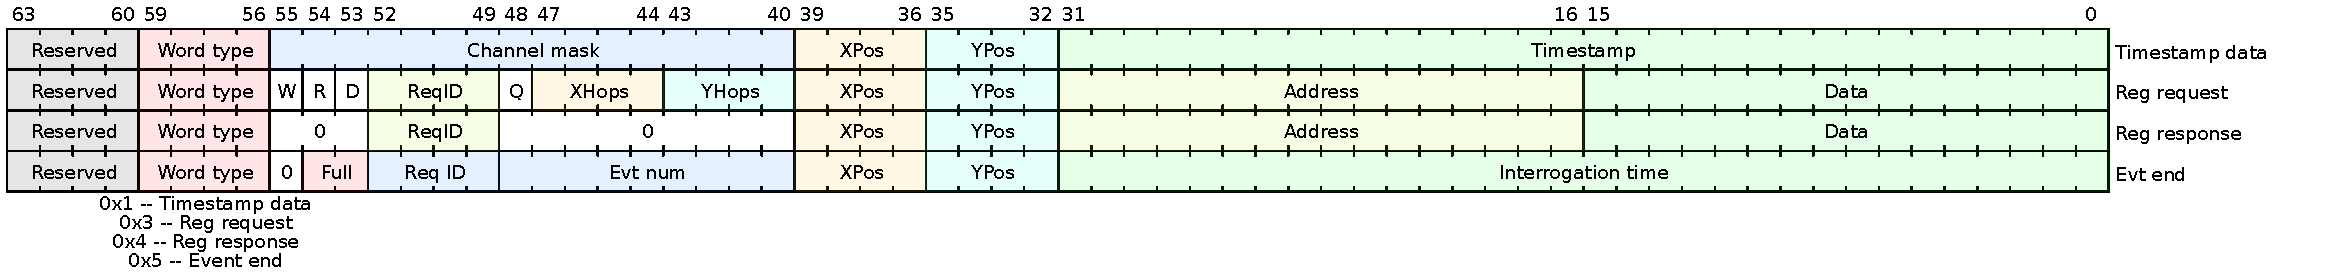
\includegraphics[width=\textwidth]{images/qpix_word_format.pdf}
\caption{Example of Datum words and their allocation as currently implemented in the simulation and first prototypes.}
\end{figure}~\label{fig:datum}

\subsection{Basic System Requirements}

The sheer number of pixels required for an APA (and the 10~\unit{kT} entire module) require an effective means of charge and time calibration, stable buffer depths, and protection against single-point failure (SPF).
Resets are records of a local counter at the current node and are recorded in response to a reset pulse sent from a pixel.

\subsubsection{Comments on Data Rates and required Computing}

Based on the minimum number of bits for each RTD~\ref{bit_calc} we can estimate minimum data rates based on tile size.


\section{The Digital Finite State Machine}

The Finite State Machine (FSM) of the remote digital ASIC outlines the designed behavior response to inputs from a controlling DAQ node.

\begin{figure}[]
\centering
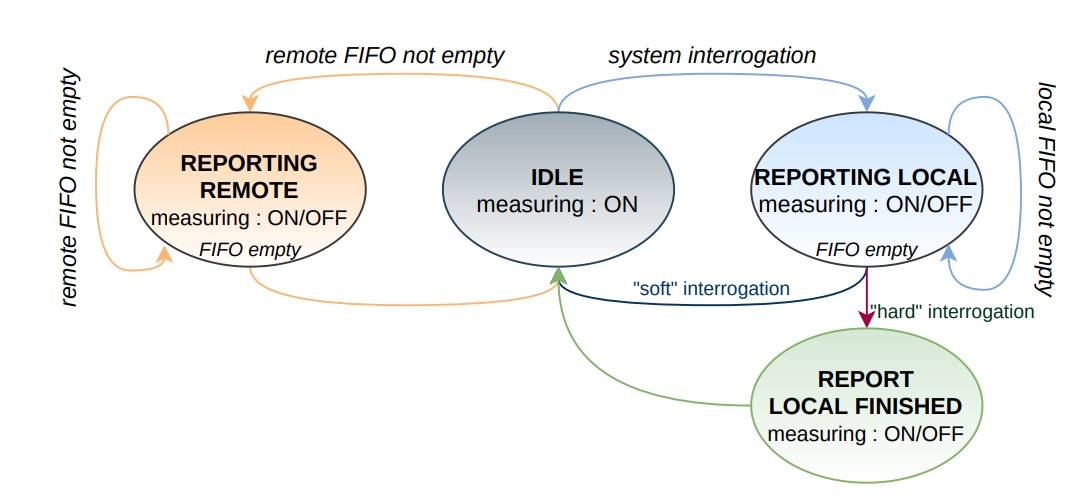
\includegraphics[width=\textwidth]{images/digital_fsm_overview.jpg}
\caption{Diagram of the Digital node's FSM which determines how to respond to incoming packets.}
\end{figure}~\label{fig:digital_fsm}

\begin{itemize}
    \item Idle, Acquisition State
    \item Transmit Local
    \item Transmit Finish
    \item Transmit Remote
    \item DONE
\end{itemize}~\label{fsm_state_labels}

\subsection{Idle}

\subsection{Transmit Data}

\subsection{Transmit Remote}


\section{The Parameter Space of the Digital System}~\label{sec:parameter_space}

The digital back-end design

\subsection{Buffer Depth Requirements}

The required buffer depth of each node in an array is the maximum number of timestamps the node can store in memory before overflow (dataloss).
Each node requires some buffer memory to record local data as well as separate storage for remote data.
The remote data which can be sent can come from any of the adjacent connected nodes, and may of any type: data words, register request, etc.
Since the remote

The ice40 FPGAs have a total of 20 Embedded Block Ram models (EBRs) which allow for a for total of 64xTODO memory depths allocated in each node.

\subsection{Endeavor Packet Stability at Different Scales}

We test two differet scales for the endeavor protocol.
This protocol maintains a relative relationship between the number of high signals used to send either a high and low bit.
The convention to send a high bit is to pulse a logic high signal for twice as long as is done for a low bit.

The number of bits used for to send a high bit are either

\begin{table}
\begin{center}
\begin{tabular}{||c c c||}
 \hline
 Name & Function & Value Range\\ [0.5ex]
 \hline\hline
  Zero & Controls how many clocks to send a logic high to transfer a low bit & 1--3 \\
 \hline
  One & Controls how many clocks to send a logic high to transfer a high bit & 2--5 \\
 \hline
\end{tabular}
\caption{The address values are not sequential because some registers have become deprecated through development.}
\end{center}
\end{table}
~\label{table:node_registers}

\subsection{The Push and Pull Architectures}~\label{sec:architectures}


\section{The Digital Back-end problem}

The main objectives of the digital back-end are to correctly measure the data presented to it by the analog front-end and ensure lossless transport of that data to disk.
More simply, the goals of the digital portion of the Q-Pix readout are to record and send data.
We note that the successful completion of these two objectives to be goal of these simulation studies.

\subsection{The Basic Datum}

We begin with a discussion of the basic datum and mention initial design choices at the physical connection interface.
The structure of this datum determines the buffer widths and depths required to store the data at the local ASIC level as well as the protocol used to transfer this data between ASICs and eventually out of the detector.

The minimum data which needs to be recorded are the timestamp, the relative location of the digitizing ASIC within the detector, plus any channels which were responsible for this reset.
Each of the number of bits assigned to recording these parameters are a design consideration.
We choose the number of bits for the timestamp ($N_{T}$) to be 32, which prevents frequency wrap-around based on a fast clock frequency (Equation~\ref{{eq:tloop}}).
We choose as the number of bits to assign a location ($N_{loc}$) to be 8, which provides a maximum possible number of unique positions before aggregation to be 256.
Next, since the number of pixels (required by analog front-end design) is 16 we choose this number as the number of bits to represent a ``mask'' ($N_{bits} = 16$).
We need to record all of the channels during each reset since it is technically possible (even if less likely) for multiple analog channels to provide a reset within the same clock window.

We calculate the minimum number of bits per datum to be:
\begin{equation}
  N_{bits} = N_{T} + N_{pix} + N_{loc} = 32 + 16 + 8 = 56
\end{equation}~\label{eq:nbits_datum}

Since buffer memory addresses and widths are normally characterized by powers of two, we can construct the basic datum size above the minimum number of bits provided by~\ref{eq:nbits_datum} to get $N_{datum} = 64$.
The remaining bits are useful for constructing different types of packets to be used by the digital ASICs for additional uses such as register configuration or to provide packet identification.

\subsection{Communication of the Datum}~\label{sec:comms}

There exist many asynchronous protocols of communication of digital information.
Most of the differences between protocols exist based on the number of connections between devices and whether or not one pin is allocated to share a clock, etc.

Our design considerations for this readout include reduction of SPF risk, low power, and minimal routing.
Partly for these reasons, the design choice for communication relies on only two connections between ASICs.
One connection is defined as a data receiver (Rx) and the other as a data transmitter (Tx).
This choice of interface dramatically limits a choice of possible protocols.
Here, we describe the difference between two that we tested: Universal Asynchronous Receiver-Transmitter (UART) and Endeavor.
We discuss and test only these two protocols for simplicity, and find it instructive to compare a proven and custom protocol (Endeavor) with a very common one (UART).

The importance of choosing a correct protocol is to ensure lossless data transmission.
Since there are free running clocks, an asynchronous communication protocol is required.
The way to ensure that data can be moved between clocks of different speeds is to stretch the signal or to repeat bits.
The more the word is stretched in time, the larger the allowable difference in frequency between the two devices.
However, this lengthening can't proceed forever, obviously, otherwise data transmission time could exceed data capture rates.

It is another important design consideration, then, to ensure that transactions proceed as quickly as possibly without data loss.
Additional concerns of long data transactions include the use of more clock cycles which use more power and increase the risk noise to leak to the analog front-end.

%% appendix??
\subsubsection{UART}~\label{sec:uart}
This common protocol is typically stable between devices with a maximum difference of clock frequency to be 10\%.

% \begin{tikztimingtable}[%
%     timing/dslope=0.1,
%     timing/.style={x=5ex,y=2ex},
%     x=5ex,
%     timing/rowdist=3ex,
%     timing/name/.style={font=\sffamily\scriptsize}
% ]
% \centering
% % \busref{$CLK_{base-tx}$} & 0.10L 156{.1428570c} \\
% % \busref{$CLK_{base-rx}$} & 0.35L 156{0.12857c} \\
% \busref{$CLK_{tx}$} & 0.10L 20{c} \\
% \busref{$CLK_{rx}$} & 0.35L 22{0.9c} \\
% \busref*{Tx} & 0.10L 2u 1D{START} 10d{DATA} 1D{STOP} 2U \\
% \busref*{Rx} & 0.35L 1.80u 0.9D{START} 10.8d{DATA} 0.9D{STOP} 1.8U \\
% \extracode
% \begin{pgfonlayer}{background}
% \begin{scope}[semitransparent ,thick]
% \vertlines[darkgray,dotted]{0.10,1.10,...,2.1}
% \vertlines[black,solid]{0.35,1.25,...,10.25}
% \end{scope}
% \end{pgfonlayer}
% \end{tikztimingtable}~\label{tikz:uart}
% wavedrom - improvement to avoid difficult tikz

%% appendix??
\subsubsection{Endeavor}~\label{sec:endeavor}

This protocol is slower than UART, but allows for approximately double the frequency difference: $\approx$ 20\%.

The endeavor protocol relies on repeating the value of a high-bit, (digital '1' value) for an integer number of clock cycles.
The receiver continually samples in incoming data transmission and counts the number of clock cycles that the signal was high for.
The longer the signal was high, the more likely it is the the transmitter was attempting to encode a high bit, and vice verse.

The number of clock cycles which accompany either a high bit transmission or a low bit transmission then represent a possible design choice for the protocol.
The actual number of bits which should be used ultimately depend on the similarity of the frequency between adjacent digital channels; the more similar the frequency (and relative phase) the lower these numbers can be.

\begin{itemize}
    \item Start Bit
    \item High Bit
    \item Low Bit Send
    \item Stop Bit Send
\end{itemize}\label{item:endeavor}

%% This section should reference how Q-Pix fits into a DUNE APA as a design goal
\section{Constraining the Digital-Backend Design}

Section~\ref{sec:qpix_apa} describes in detail how a Q-Pix based hardware readout architecture could fit within a single DUNE-APA.
Here we extend this discussion and use those constraints as the starting point for a search for a solution to the digital back-end architecture.
The first problem to solve is how to aggregate the all timestamp data supplied by the large number of channels within a DUNE-FD APA.

A Q-Pix architecture would likely use either a high-performance FPGA or a custom ASIC to aggregate the large number of $(\mathcal{O}(10^{7})$ channels.
The number of aggregated digital channels determines the required capabilities of the aggregator node and the selection of an FPGA or ASIC.
Since each additional aggregator node represents an additional SPF risk, our design goal suggests that the optimal configuration is one that produces the least number of aggregator nodes.
Therefore, the goal is to design a routing architecture which is responsible for as many digital channels as possible for each data aggregator node which still allows for accurate timing calibration and lossless data acquisition.

However, as one increases the number of digital channels per aggregator node one also increases the amount of local oscillators per aggregator, each of which must be calibrated.
Additionally, since each digital channel requires extra communication time (as discussed in section~\ref{sec:comms}) the introduction of more channels negatively affects the precision of timing calibrations and potentially increases SPF risk of digital channels.
We consider then that an optimal number of digital channels per aggregator node is one that maximizes the number of digital channels but still maintains the required timing calibration~(Sec.~\ref{sec:background}) and transmits lossless data.

We refer to the total number of digital channels collected from one pathway to an aggregator as a tile.
In a fully realized design an aggregator might in fact be responsible for multiple tiles, which need not necessarily be the same size.
The requirements of an aggregator node is completely determined by the composition of tiles it is connected to.
Then, a parameteriziation of the data requirements imposed by each tile can be extended to describe the requirements of the aggregator node.
Finally, we reach the conclusion that the required parameterization of the back-end system relies on the parameterization of the tile.

A tile is composed of inter-connections between digital channels.
The LArTPC design suggests that each digital channel have a maximum of four connections since the collection of charge happens on a flat two-dimmensional anode plane.
Therefore, a two-dimensional routing requires at least two independent communication channels, which if we require the digital channels to allow bi-directional communication, the minimum number of channels is four.
We use this number as a starting point for the digital channel design.
These four connections per channel immediately creates a rectangular connection structure for a tile.

% once aggregator is selected, hardware can be parameterized
We note here that in order to meet other physical design requirements to fit into a pre-existing APA frame, the capability of the aggregator nodes could be increased to be responsible for more tiles, which would reduce the cable and hardware engineering considerations.
However, further consideration here is beyond the scope of this work.

% tile connection methods
\subsection{Tile Routing Considerations}

A tile is a rectangular composition of digital channels which must provide a path to all digital channels and send lossless data to the aggregator.
Since there is one connection between a tile and the aggregator, there is one special node within the tile that connects to the aggregator.
This special node we refer to as the ``base-node'' as all data and instruction commands, regardless of routing, must pass through this node.
The symmetry of the rectangular tile allows any corner node to be the base node, and we choose the upper-left to define a convention.
An example of a tile with a Corner base-node is shown in Figure.~\ref{fig:cbn}.

We do not consider possible configurations where an aggregator might be connected to a digital channel within a tile since we require that all digtal channels are identical and fully connected.
We require identical channels as a practical choice due the required number of total channels.
We also require the tile to be fully connected to allow as many possible unique paths between the base-node and the other nodes which provides maximum protection against SPF.
We address that we discuss why we do not consider base-nodes placed on the outter edge of a tile, but not at the corners more generally in section~\ref{sec:base_node}.
Briefly, base-nodes which are along the outter edge of a FCT but not at the corners simply contain two sub-graphs of FCT with a base-node along the edge.
Therefore, an analysis of the constraints of a FCT with corner base-nodes can be mapped to an analysis of FCT with edge base-nodes.

\begin{figure}[]
\centering
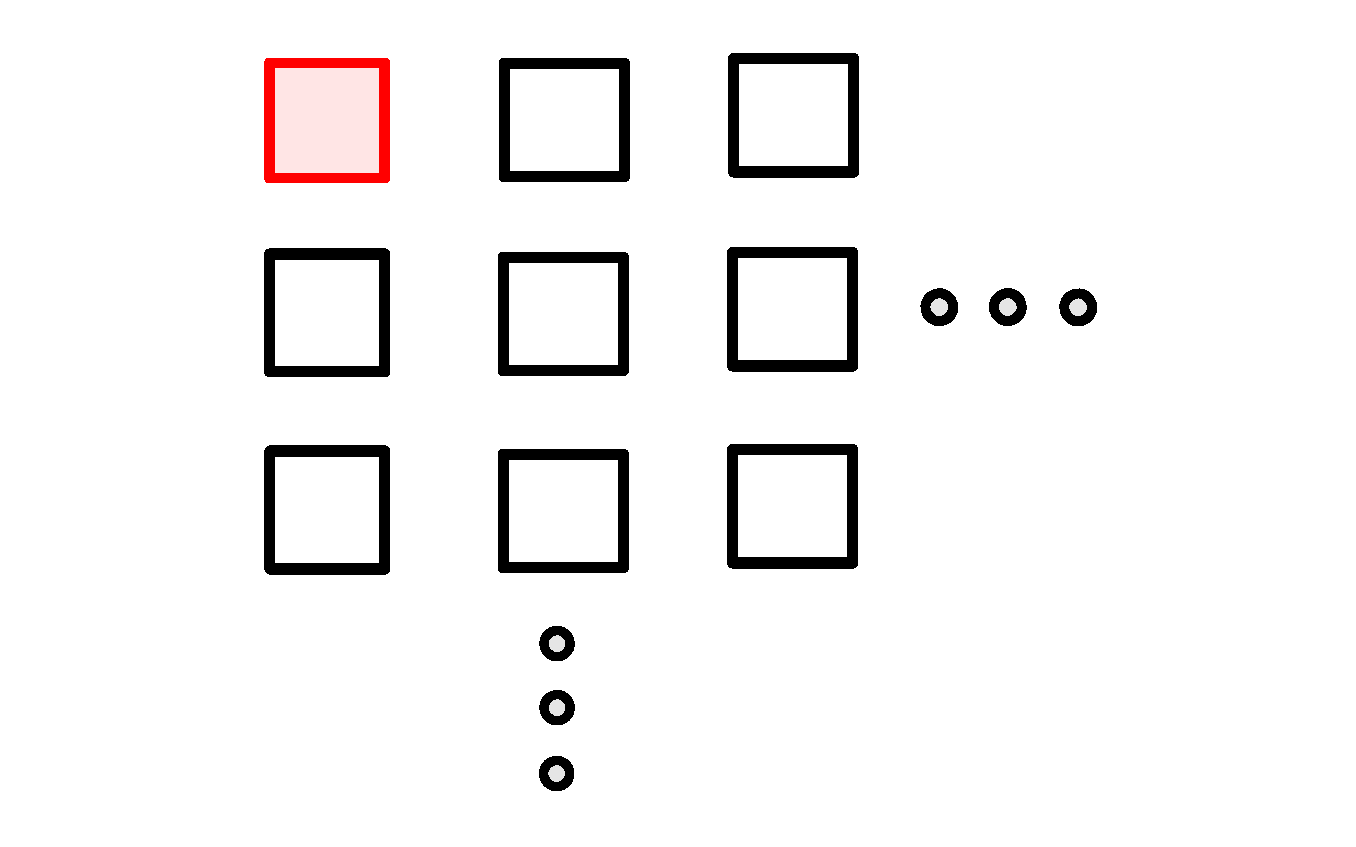
\includegraphics[width=\textwidth]{images/CBN.pdf}
\caption{Example of an Corner Base-Node configuration. The base-node is colored and highlighted in red.}
\end{figure}~\label{fig:cbn}

Here we introduce a particular representation (based on graph-theory) for a tile which is useful for simplifying simulations and for analyzing particular routing configurations.
The most general tile configuration occurs when we assume that all adjacent nodes within the tile are connected; this creates what we refer to as a ``fully connected tile'' (FCT).
An example of a FCT is shown in Figure~\ref{fc_tile}.
Any particular choice of an effective routing must then be a subset of this fully connected version.

\begin{figure}[]
\centering
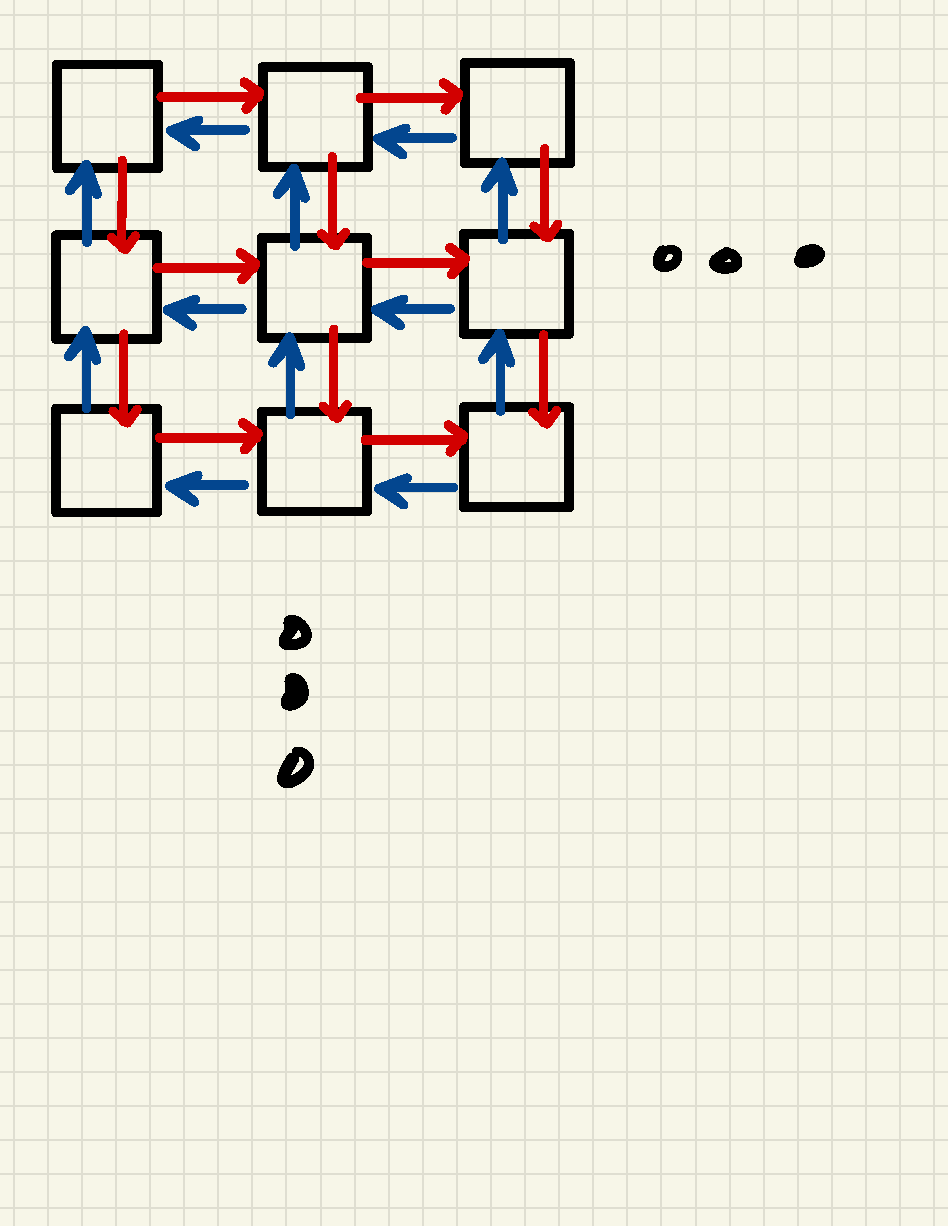
\includegraphics[width=\textwidth]{images/Notes.pdf}
\caption{Example of the fully connected routing configuration for a tile (FCT). Each Node represents a digital channel which must be aggregated, and the red and blue connections distinguish directions of communication. The red connection lines indicate pathways away from the base node, whereas the blue lines represent connection paths towards the base-node in the upper-left.}
\end{figure}~\label{fig:fc_tile}

To elaborate on the adjacency matrix of the FCT we consider an $2\times 3$ tile.
A $2\times 3$ tile has six total nodes, where we consider the upper-left most node to be the base node.
Then, the unweighted adjacency matrix has dimensions $6\times6$ of the form:
\begin{equation}
M =
 \begin{pmatrix}
 0 & 1 & 0 & 1 & 0 & 0 \\
 1 & 0 & 1 & 0 & 1 & 0 \\
 0 & 1 & 0 & 0 & 0 & 1 \\
 1 & 0 & 0 & 0 & 1 & 0 \\
 0 & 1 & 0 & 1 & 0 & 1 \\
 0 & 0 & 1 & 0 & 1 & 0 \\
 \end{pmatrix}
\end{equation}~\label{eq:adjacency_matr}


Where each non-zero value of $M_{ij}$ represents a connection between nodes $i$ and $j$.
As an unweighted, undirected graph this is a symmetric matrix.

In practice each digital channel within a tile is actually controlled by a unique, free-running oscillator.
Therefore, we can define the length of each edge between nodes as the length of time to send of a packet of data between two nodes ($T_{i\rightarrow j}$).
With this we can extend the model the adjacency matrix as a weighted and directed graph if we recognize that the non-zero elements of $M_{ij}$ become $T_{i\rightarrow j}$, or the length of time it takes for the $i^{th}$ local oscillator to transmit a packet to node $j$.

We can generalize this matrix in terms of an arbitrary number of rows ($r$) and columns ($c$).
We define a convention of numbering nodes within the tile in terms of increasing column number followed by increasing row number.
With this convention we obtain the general adjacency matrix with values defined by:
\begin{equation}
  M_{ij} = T_{i\rightarrow j}(\delta_{i,j=i\pm 1} + \delta_{i,j=i\pm r})
\end{equation}~\label{eq:adjacency_comp}

An adjacency list can similarly be constructed from Equation~\ref{eq:adjacency_comp} where the non-zero connections are given by the kroniker-deltas factors.

The length between the nodes represets the time it takes for a packet to transact from one node to the next.
This is determined by both the number of clocks to be sent in the communication protocol ($N_{bits}$) and the period of the transmitting and receiving oscillators, $T_{i}$ and $T_{j}$, respectively.
Unlike the transmitter, the receiver only affects the transaction time with a single clock cycle, as the protocls we test here, (UART and Endeavor), each conclude a packet transaction when the receiver records the last bit transaction from the transmitter.

The full length between two nodes, $i$ and $j$, connected by an edge is represented by:
\begin{equation}
T_{i\rightarrow j} = N_{bits}T_{i} + T_{j}(t)
\end{equation}~\label{eq:t_packet_full}

where $T_{j}(t)$ represents the time dependent fractional part of one nominal clock period of the receiving node.
The expectation value of $T_{j}(t)$ is half of the nominal window so that mean Equation~\ref{eq:t_packet_full} is:
\begin{equation}
\bar{T}_{i\rightarrow j} \simeq N_{bits}T_{i} + \frac{T_{j}}{2}
\end{equation}~\label{eq:t_packet_avg}

Since the transaction time of a packet is much larger than a single clock cycle ($N_{bits} \simeq \mathcal{O}(10^{2}) \gg \frac{1}{2}$), we can approximate Equation~\ref{eq:t_packet_avg}:

\begin{equation}
\bar{T}_{i\rightarrow j} \approx N_{bits}T_{i}
\end{equation}~\label{eq:t_packet}

This representation is also useful to model certain SPF where a node becomes inactive.
Dead or inactive nodes are ones in which all of their connections are effectively disconnected.
This is equivalent to setting their transaction lengths to zero: $T_{SPF} = 0$.

We comment that although it is possible to construct tiles where more than one node connects to the aggregator, we observe that this configuration simply produces two effective tiles.
These distinct tiles then are the data paths which are unique to each base-node.
In this graphical representation a packet of data can follow one, and only one path from the origin node to the base-node unless there was duplication of packets.
We emphatically avoid designs which might depend on data duplication for reduncancy; these two base-nodes are in unconnected graphs.

Additionally, it is possible to connect non-rectangular tiles, but these tiles are effectively a larger rectangular tile with disconnected nodes to produce the desired shape.
Since every node is designed to be robust in the full version, it will be be robust in the subset.

We can apply this same argument to base-nodes which do not lie at the corners of the rectangular tile.
In the case where the base-node is selected along the edge
Therefore, we conclude that the analysis of the tile with the above adjacency matrix and a selection of the base-node at the corner of a rectangular corner provides the basis problem to the tile configuration.

\subsubsection{The SPF Cost}~\label{sec:spf_cost}

We define the average SPF cost as the amount of nodes that will be lost during a transaction as the number of digital channels at a height below the failed digital channel.
For example, the number of nodes which are lost if a leaf-node fails is one since no other channels are between it and the data node.
Likewise, the number of nodes which are lost in the event of a base-node failure is the total tile, $N$.

We can then calculate a mean cost SPF, $C_{SPF}$, :
\begin{equation}
  C_{SPF} = \frac{1}{N}\sum_{node} \frac{n_{i}}{N} = \frac{1}{N^{2}}\sum_{node} n_{i}
\end{equation}~\label{eq:cspf}

\subsubsection{Minimize Occupancy}~\label{sec:min_conn}

One of the goals of a succesful digital design is to ensure lossless data transfer.
One point of failure on the digital side is an overabudance of data arriving at a single layer within the tree.
This data loss occurs when data are sent to a node faster than the data leaves the node, and persists for long enough such that the buffers of the node overflow.
This creates a horrible loss of data which can't be recovered.

A routing scheme which minimizes the overall occupancy in the tree depths is shown in Figure~\ref{fig:snake}.
We refer to the style of routing as ``Snake''-routing (SR), because this is also the longest possible routing scheme for a square tile.

\begin{figure}[]
\centering
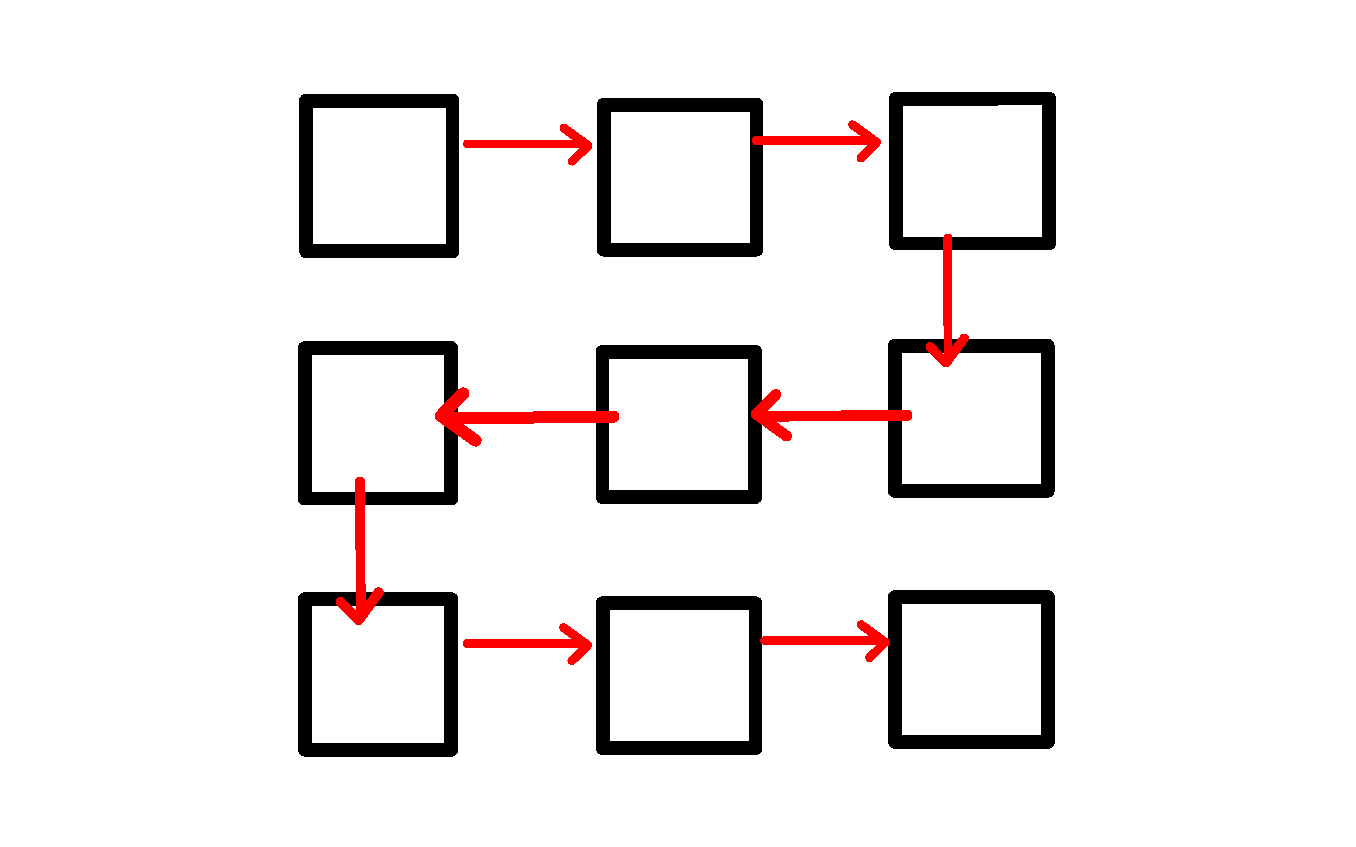
\includegraphics[width=\textwidth]{images/snakeroute.pdf}
\caption{Minimal Occupancy Path of a FCT. This routing path ensures that the number of input connections equal the number of output paths for the node.}
\end{figure}~\label{fig:snake}

We inspect the SPF risk from this routing scheme with Equation~\ref{eq:cspf}, where we notice that the $n_{i}$ of each node is simply a running sum from the leaf to $N$ at the base node.

\begin{equation}
  C_{SPF} = \frac{1}{N^{2}}\frac{N(N+1)}{2} = \frac{1}{n}\frac{N+1}{2} = \frac{1}{2} + \frac{1}{2N}
\end{equation}~\label{eq:cspf_snake}

Equation~\ref{eq:cspf_snake} tells us that the SPF risk of this routing configuration converges to half as the size of the tile grows.
Intuitively, this makes sense, since it is equally likely to select a node close to the base-node as it is far away, which implies that the sum should converge to half the tile size for large $N$.

Although this routing scheme provides the most lax constraint on the requried buffers at each digital channel, it provides the longest average path between the base node.
The longer the transaction delay between the base-node and other nodes increases the reconstruction time uncertainty.
Therefore, a natural alternative routing scheme is one that minimizes the communication scheme.

\subsubsection{Minimize Delay}~\label{sec:min_comm}

For any given node in an edge FCT with location $(R_{i},C_{i}$), the shortest path to the base-node is simply the sum of its coordinates: $R_{i}+C_{i}$.
An example of such a routing configuration for a tile is shown in Figure~\ref{fig:leftroute}.

\begin{figure}[]
\centering
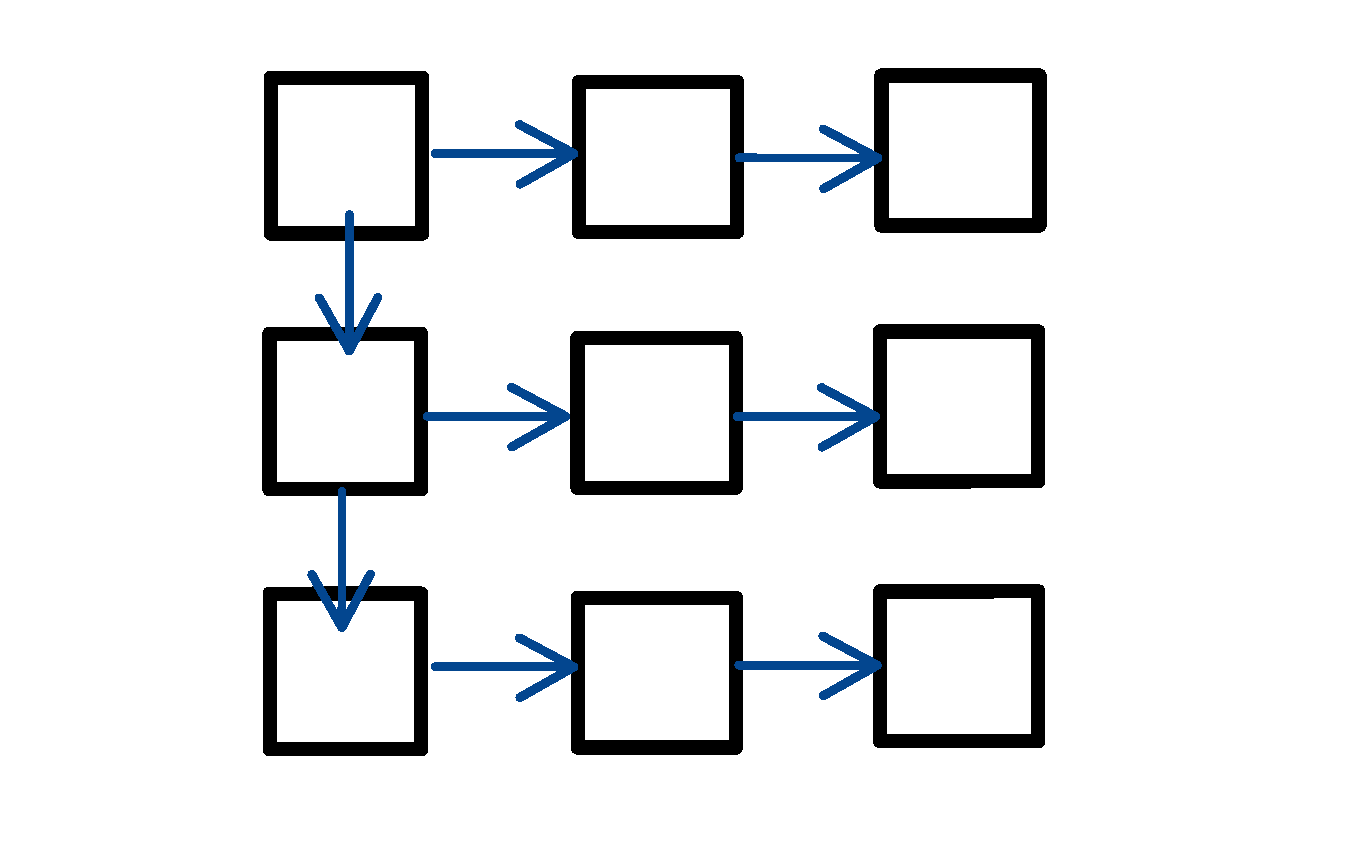
\includegraphics[width=\textwidth]{images/leftroute.pdf}
\caption{Minimal Delay Path of a FCT. This routing path ensures that the minimum number of transactions occur from every node in the FCT to reach the base-node. For any node along any column this is equivalent to the sum of the row and column of that node.}
\end{figure}~\label{fig:leftroute}

We can calculate $C_{SPF}$ for this routing configuration if we identify that there are a $C$ number of rows which sum from one to $R-1$.
Likelise, the far-left column in Figure~\ref{fig:leftroute} shows that the number of rows, $R$, sum from one to $C$.
We can rewrite the sum over all nodes in Equation~\ref{eq:cspf} as:

\begin{equation}
  \sum_{node}n_{i} = C\sum_{i=0}^{i=R-1}i + R\sum_{i=0}^{i=C}i
\end{equation}~\label{eq:cspf_left_s}

We simplify the running sum of each term in Equation~\ref{eq:cspf_left_s}:
\begin{equation}
  \sum_{node}n_{i} = C\frac{R(R-1)}{2} + R\frac{C(C+1)}{2} = RC(\frac{R+C}{2})
\end{equation}~\label{eq:cspf_left_e}

Using this result we obtain $C_{SPF}$ by identifying $N = RC$:
\begin{equation}
  C_{SPF} = \frac{1}{N^{2}}\sum_{node}n_{i} = \boxed{\frac{R+C}{2RC}}
\end{equation}~\label{eq:cspf_left_fin}

This result informs that relative cost of losing a node tends to zero as the size of the tile grows.
Again, this result can be obtained intuitively, since as the number of columns (or rows) grow in size, the probability of a single failure occuring on the aggregator column is increasingly less likely.


\subsubsection{Broadcasts to avoid SPF}~\label{sec:broadcast}

In order to protect against SPF we only consider a designs which implement the FCT, since SPF can occur on any node the most robust connection scheme is the FCT.
A FCT allows searches to probe all possible paths to any node via a ``broadcast'' produced from packets sent by the aggregator to the base-node.
Therefore the broadcast algorithm can be represented by a complete circuit which begins at the base-node and proceeds to a target node with no repeated nodes until the target node is reached.
The backward path is then completed in reverse by following the edges (connections) between each node until arriving finally again at the base-node.

In practice, we encode the broadcast packet with a special header, to separate it from a request packet, and include an identification number.
Then, any node which receives a broadcast packet will record the identification number of the most recent broadcast, which it can use to discard additional broadcast packets that arrive with the same number.

In the event that a particular node becomes inactive it will ``block'' data comming from the nodes along its path.
In this case, there must be some sort of ``broadcast'' originating from the base-node that would allow information tranverse regardless of the effective routing path.

%% colored matrix
\def\r{\color{red}1}
\def\b{\color{blue}1}
\begin{figure}[h]
  \begin{tabular}{p{5cm}c}
    {${\renewcommand{\arraystretch}{2.0}}
        \begin{pmatrix}
          0 & \r & 0 & \r & 0 & 0 \\
          \b & 0 & \r & 0 & \r & 0 \\
          0 & \b & 0 & 0 & 0 & \r \\
          \b & 0 & 0 & 0 & \r & 0 \\
          0 & \b & 0 & \b & 0 & \r \\
          0 & 0 & \b & 0 & \b & 0 \\
        \end{pmatrix}$}
    &
    $\vcenter{\hbox{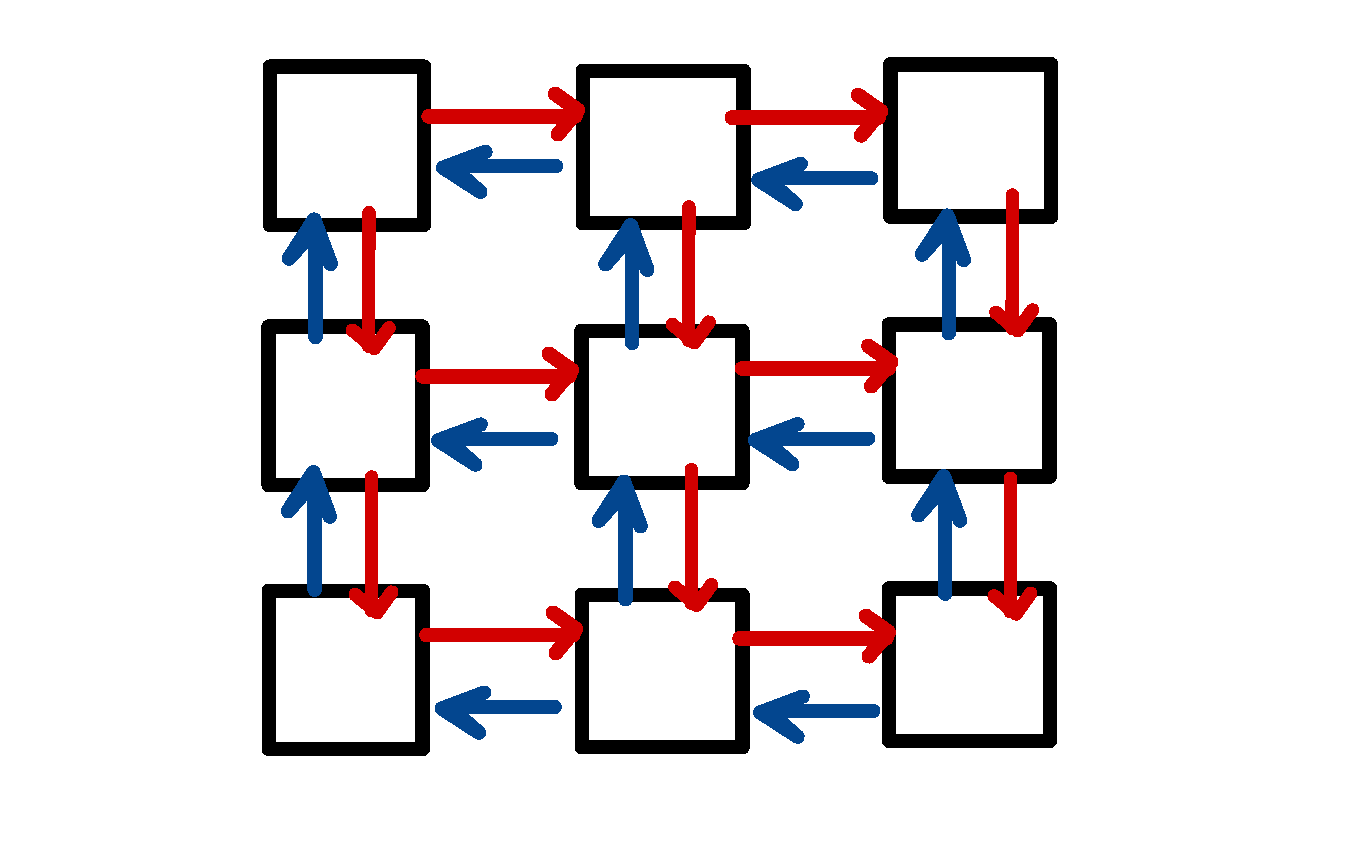
\includegraphics[scale=0.5]{images/Broadcast.pdf}}}$
  \end{tabular}
\caption{Minimal Routing Path of a FCT. This routing path ensures that the number of input connections equal the number of output paths for the node.}
\end{figure}~\label{fig:FCT_colored}

\subsection{Comments on the Edge Base-node and Other Routings}~\label{sec:base_node}

We discuss here the case of a FCT with an edge base node.
An edge base node (EBN) is a digital channel that connects to the aggregator and to three other digital channels within a tile.
Like before, this base-node must provide a unique path during data transmission to all digital channels within the tile.
In this configuration the adjacency matrix is still the same as given in Equation~\ref{eq:adjacency_comp}.

Also, as before, we wish to inspect different routing scenarios for a tile of a given square dimension of $R$ rows and $C$ columns.
We can proceed by dividing the FCT graph into two subgraphs, $S1$ and $S2$, where $S1$ represets the rectangular section of the graph below and to the left of the EBN, while $S2$ are the remaining channels.

We identify that while the number of columns ($C$) in tile is equal to both subgraphs, the total number of rows $R$ of the tile is equal to the sum of the rows from these two subgraphs: $R = R_{1} + R_{2}$.

\begin{figure}[]
\centering
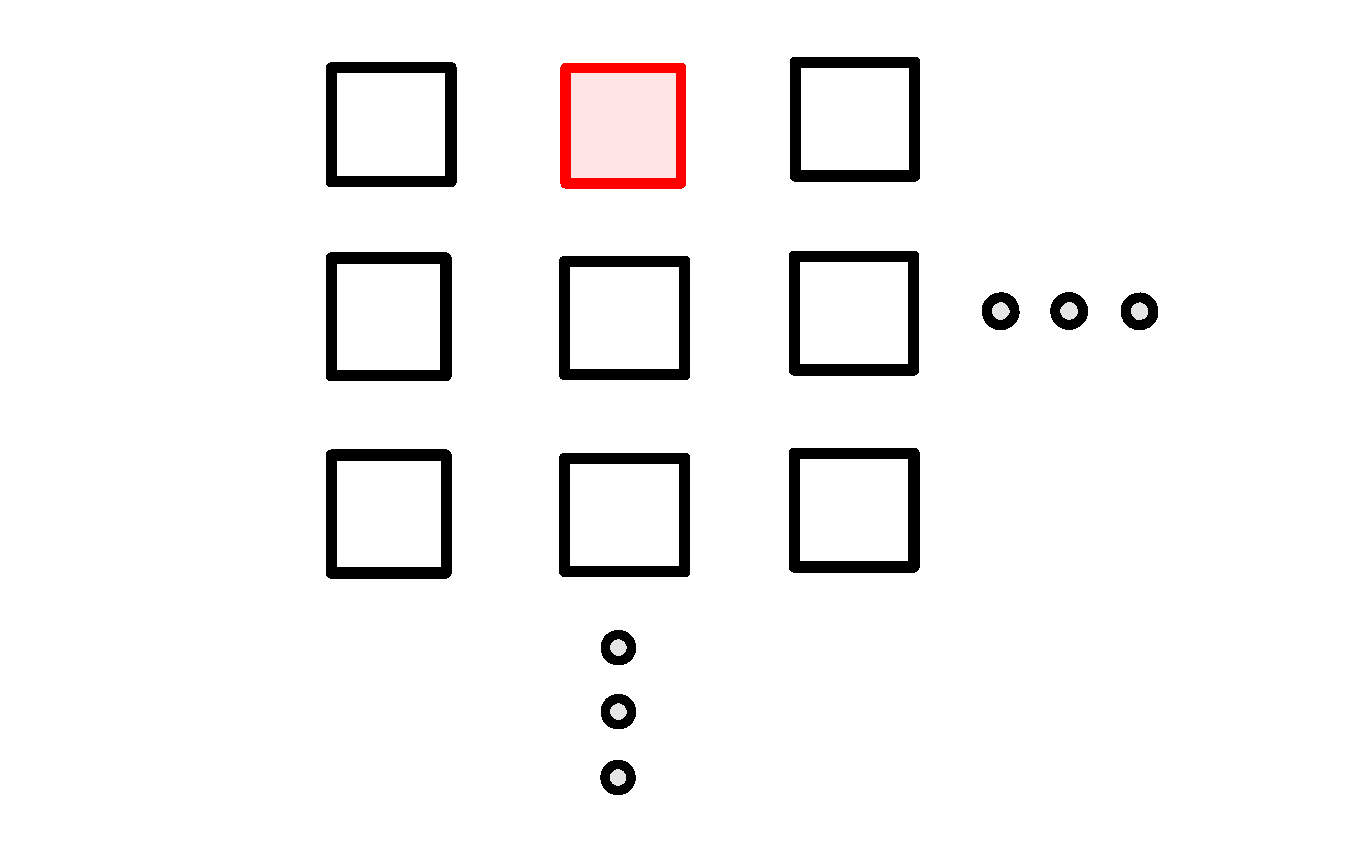
\includegraphics[width=\textwidth]{images/EBN.pdf}
\caption{Example of an Edge base-node configuration. The base-node is colored and highlighted in red.}
\end{figure}~\label{fig:ebn}

% \begin{tikzpicture}[->,>=stealth',shorten >=1pt,auto,node distance=1.25cm,
%                     ,auto=center]
%                     % ,auto=center,every node/.style={circle,fill=blue!20}]
%   \tikzstyle{every node}=[fill=blue,draw=none,text=white]

%   \node (1) at (0,0) {1};
%   %% row 1
%   \node (2) at (1,-1) {2};
%   \node (3) at (2,-2) {3};
%   \node (4) at (3,-3) {4};
%   % row 2
%   \node (5) at (0, -1) {5};
%   \node (6) at (1,-2) {6};
%   \node (7) at (2,-3) {7};
%   \node (8) at (3,-4) {8};

%   %% end nodes
%   \node (10) at (0, -5) {$C$}; % must be at 0 x
%   \node (11) at (5, -5) {$R$}; % must be 1:1 slope
%   \node (12) at (5, -10) {$R+C$}; % must be 1:1 slope

%   %% paths
%   % \path (4) -- (11) [red, midway, sloped] {$\dots$};
%   % \path (5) -- (10) [red, midway, sloped] {$\dots$};
%   \draw[red,thick,dashed] (4) -- (11);
%   \draw[red,thick,dashed] (5) -- (10);
%   \draw[red,thick,dashed] (10) -- (12);
%   \draw[red,thick,dashed] (11) -- (12);

%   \path (1) edge (2);
%   \path (1) edge (5);
%   \path (2) edge (3);
%   \path (3) edge (4);
%   \path (5) edge (6);
%   \path (6) edge (7);
%   \path (7) edge (8);
% \end{tikzpicture}

The EBN then is actually just a composition of two subgraphs which are each equivalent to The tree characteristics which determine requirements for the digital channels are the tree height and total occupancy at each level.
Therefore, since the EBN provides no difference in either of these characteristics and is a suposition of two fundamental CBN, an analysis of an EBN is equivalent to the analysis of a CBN.

However, we do remark comment that the average difference of the relative weights of each node in a SPF analysis are different in a EBN compared to the CBN case.
This should be obvious since the relative weight of each node is determined by the running sum of the path length betwee the base-node and its leaf.
For a fixed row dimension, $R$, the EBN offers a smaller average tree height for each of its componet radia $R_{1}$ and $R_{2}$.

Therefore, in a EBN tile, with two subgraphs of radii $R_{1}$ and $R_{2}$ where the base-node is on the $R_{1}$ edge.
The total sum of the weights of all nodes in the tile are the sums of the two subgraphs plus $CR_{2}$, which is the average weight of the nodes from the subgraph $R_{2}$ when it connects to $R_{1}$.
\begin{equation}
  \sum_{node}n_{i} = \sum_{R_{1}} + \sum_{R_{2}} + CR_{2}
\end{equation}~\label{eq:cspf_ebn}

Equation~\ref{eq:cspf_ebn} gives the general formula for calculating the SPF risk for a EBN case, depending on the routing methods of subgraphs $R_{1}$ and $R_{2}$.
We can treat these sub-graphs as in equation~\ref{eq:cspf_left_fin} to obtain:
\begin{equation}
  \sum_{R_{1}} + \sum_{R_{2}} + CR_{2} = \frac{R_{1}C(R_{1}+C)}{2} + \frac{R_{2}C(R_{2}+C)}{2} + CR_{2}
\end{equation}~\label{eq:cspf_e}

We use this result to obtain the relation of the general $C_{SPF}$:
\begin{equation}
  C_{SPF} = \frac{1}{N^{2}}(\frac{R_{1}C(R_{1}+C)}{2} + \frac{R_{2}C(R_{2}+C)}{2} + CR_{2})
\end{equation}

if we identify that $N = C(R_{1}+R_{2})$ and use $R_{2} = R - R_{1}$:
\begin{equation}
  C_{SPF} = \frac{1}{2CR^{2}}(2R_{1}^{2}-2R_{1}R+R^{2}+CR+2(R-R_{1}))
\end{equation}


\section{Frequency Calibration of Local Oscillators}~\label{sec:calib}

The Q-Pix calibration requirements are described in detail in Section~\ref{sec:qpix_calib}.
The important parameters which must be calibrated for each pixel are the charge per reset and the frequency of the local oscillator.
An aim of this work is to demonstrate an additional frequency calibration method using the minimal required connections between each digital node.

Any method of a frequency calibration must synchronize time measurements between all digital nodes within a tile and the aggregator.
There are several possibile methods to achieve this, but ultimately the data that are recorded must be some time at the aggregator, $T_{a}$, and the time at any specific node, $T_{j}$.

%% distribute clock for calibration of time
A direct method is one where the aggregator distributes its own clock to all nodes in the tile.
This scenario removes the need for a calculation of the frequency of each node altogether since the clock of each node is already known from the aggregator.
This is the simplest case for timing calibration: remove all free running oscillators.
However, this method also introduces complex routing and power requirements within every tile.

% TODO
% cross-talk
A distributed clock network indeed removes ambiguity of the remote oscillator frequencies, but at the cost of hardware complexity.
Whether or not this design choice is preferred is entirely detector dependent, but likely increases in difficulty with the scale of the TPC.

We comment, however, that we ignore this scenario because it may altogether be unnecessary depending on future ASIC performance.
In the event that frequency calibrations of sufficient precision ($\bar{f} \approx 1 ppm$) are possible occur on free-running local oscillators future detectors would need only to acquire these ASICs and place them with minimal cost in terms of both time and money.

%% distribute trigger for calibration of time
Another simple scenario is one where the aggregator itself connects directly to all nodes within a tile via a single connection which can be used as a reference trigger.
This means that some trigger from the aggregator would issue directly into each node at the same time: $T_{a} = T_{n}$.
To calcuate the frequency in this manner, the controller would issue two triggers from the aggregator with a known time separation, $T_{o} = T_{a2} - T_{a1}$.
The remote nodes would each record and send their timestamps back to the aggregator, where the time difference would be calculated as:

\begin{equation}
  T_{o} = T_{a2} - T_{a1} = T_{n2} - T_{n1}
\end{equation}

this is rewritten in terms of frequency as follows:
\begin{equation}
  f_{n} = \frac{T_{n2} - T_{n1}}{T_{o}}
\end{equation}

This calibration method extremely simple but introduces an additional connection to each node between itself and the aggregator.
For a large scale system such as Q-Pix even this simple connection scheme introduces $\approx 60\times 10^{3}$ hardware points of failure per APA.

Both of these scenarios are valid implementations of a Q-Pix readout system.
In both of these scenarios, however, there is added complexity into the hardware design of the system in the form of additional routing where each route which represents a possible point of failure.

In a world of perfect hardware and costless routing in terms of both time and money these routing schemes would clearly be sufficient.
However, no hardware is perfect.
Therefore we introduce and discuss a calibration technique which relies on no additional routing and could be optionally implemented even in the above schemes in the event of a failure.
Therefore, even if not the primary implemented calibration technqiue, since this calibration introduces no superfluous routing it could still be used regardless of the actual future hardware implementation.

%% distribute packet for calibration of time
\subsection{A Minimal Connection Calibration Procedure}~\label{sec:min_calib}

As stated in the previous section, any frequency calibration records a reference time at the aggregator ($T_{a}$) and an event time ($T_{n}$) at a node within a tile.

the time calibration procedure presented here requires only the minimal routing required in any Q-Pix readout system, where we assume time-dependent free-running local oscillators at each node within the tile.

%% issue 1
The calibration procedure begins at a time ($T_{0}$) where the aggregator sends a calibration packet.

%% recv1
Next, the packet propagates through the tile to some remote node, $N_{j}$.
This node receives the packet later at some time $T_{n1}$:

\begin{equation}
  T_{n1} = T_{o} + T_{f1}
\end{equation}

Where $T_{f1}$ is the propogation time of the packet from the aggregator to the $N_{j}$ node.

%% meas1
This remote node then sends the packet with its time ($T_{n1}$) back to the aggregator.

%% wait
The aggregator will wait some calibration time ($T_{cal}$) before issuing another calibration packet.
This wait period $(\mathcal{O}(10^{0-2})$) can be long compared to the full transaction time to the $N_{j}$ node $(\mathcal{O}(j*10^{-5})$).

%% issue 1
After the wait period, the aggregator will issue a second calibration packet to be sent to a remote node at time:
\begin{equation}
  T_{1} = T_{cal} + T_{0}
\end{equation}

%% recv2 and meas2
Similarly to the first packet this packet will propagate to $N_{j}$ with some new time $T_{f2}$ where $N_{j}$ will record time $T_{n2}$:
\begin{equation}
  T_{n2} = T_{1} + T_{f2}
\end{equation}

Now, we define $\Delta T_{j}$ as the difference in the two time measurements from the two packets sent from the aggregator.
The time difference is related to the number of clocks that occured between the two different measured values of the clock, $T_{n1}$ and $T_{n2}$.

\begin{equation}
  \Delta T_{j} = T_{n2} - T_{n1}
\end{equation}

We use the known relationships for $T_{n2}$ and $T_{n1}$ to obtain:
\begin{equation}
  \Delta T_{j} = (T_{1} + T_{f2}) - (T_{o} + T_{f1}) = (T_{1} - T_{0}) + (T_{f2} - T_{f1}) = T_{cal} + \Delta T_{f}
\end{equation}

Where we defined $\Delta T_{f}$ as the difference in forward propagation times from the packets sent from the aggregator node at $T_{1}$ and $T_{0}$.

We arrive at the result which compares the measured time at the aggregator $T_{cal}$ and the time measured at each node, $\Delta T_{j}$:
\begin{equation}
  \Delta T_{j} = T_{cal} + \Delta T_{f}
\end{equation}

A perfect reconstruction of the nodal frequency would follow if $\Delta T_{f} = 0$.
But it is sufficient to note that the wait period happens on the order of seconds, whereas $\Delta T_{f}$ is on the order of $\mu s$ or at least a six order of magnitude difference.
We then use $\Delta T_{f} \ll T_{cal}$ to obtain:
\begin{equation}
  \Delta T_{j} \approx T_{cal}
\end{equation}

We convert time into frequency with the difference of the timestamps measured and a known aggregator frequency ($f_{a}$):
\begin{equation}
   \frac{\Delta N_{j}}{f_{j}} = \frac{\Delta N_{a}}{f_{a}}
\end{equation}

or,
\begin{equation}
   \boxed{f_{j} = \frac{\Delta N_{j}}{\Delta N_{a}}f_{a}}
\end{equation}

Where $\Delta N_{j}$ and $\Delta N_{a}$ are the differences in the timestamps of the 32-bit clocks at the remote node and aggregator, respectively.


\subsubsection{Packet Transaction Time}

 We next examine the approximation that $\Delta T_{f} \ll T_{cal}$ and consider its contribution to the error in the reconstruction of $T_{j}$.
This analysis also provides a constraint on the duration of $T_{cal}$ to ensure an accurate measurement of each $T_{j}$ in a tile.
We begin by discussing how long it takes for a packet to traverse a tile.

The time it takes for each packet to be received by the next node is given in Equation~\ref{eq:t_packet}.
The value, $N_{bit}$, is the number of clock cycles used for the packet and is protocol-dependent.
Since the protocol must be deterministic for each packet, $N_{bits}$ must be the same for each transaction on the path from the base-node to the remote node.

As an example, the time it takes for a packet to go from the base-node, $N_{1}$, to a remote node, $N_{3}$, via the path $1\rightarrow 2 \rightarrow 3$ is determined by:
%% packet transaction time
\begin{equation}
  T_{1\rightarrow 3} = T_{1\rightarrow 2} + T_{2\rightarrow 3} \approx \frac{N_{bits}}{f_{1}} + \frac{N_{bits}}{f_{2}} = N_{bits}(\frac{1}{f_{1}} + \frac{1}{f_{2}})
\end{equation}~\label{eq:t_packetTransfer}

Where, $f_{i}$, is the frequency of the clock at sending node. The approximation is within a single clock cycle of the receiving digital node ($\approx 33~\unit{ns}$).

Therefore the time it takes for a packet for go from the base-node to any remote node is proportional to $N_{bits}$ multiplied by the sum of the edges in the full adjacency matrix given by Equation~\ref{eq:adjacency_comp}.

We generalize Equation~\ref{eq:t_packetTransfer} to represent the time it takes a packet to go from the aggregator ($i = 0$) to any remote node, $N_{j}$:
\begin{equation}
  T_{f} = T_{0\rightarrow j} = N_{bits}\sum_{i=0}^{i=j-1}\frac{1}{f_{i}}
\end{equation}

We require that every calibration packet on the protocol uses the same number of clocks ($N_{bits}$ is constant) and follows the same path. $\Delta T_{f}$ becomes:
\begin{equation}
  \Delta T_{f} = N_{bits}\sum_{i=0}^{i=j-1}\frac{1}{\Delta f_{i}} = N_{bits} \sum_{i=0}^{i=j-1}\Delta T_{i}
\end{equation}

We recognize $\Delta T_{i}$ as the nominal time-dependent clock drift of the each local oscillator in the path between the base-node to the remote-node.
We can provide an order of magnitude estimate for $\Delta T_{f}$ if we assume a (very poor) $\approx 1\%$ drift in each of the remote clocks within the tile during a period of $T_{cal} \approx 1~\unit{s}$.
In this approximation we also assume that the mean of the periods of the nodes are the designed value ($\approx 33~\unit{ns}$) for which a 1\% error gives $\sigma_{T_{f}} \approx 3~\unit{ps}$.
If we assume that all of the clocks (for whatever reason) drift have error which drifts int he same direction (the sum doesn't cancel) then for 100 transactions with 1000 clocks per transaction, we obtain for $\Delta T_{f}$:
\begin{equation}
  \Delta T_{f} \approx 1000 * 100 * 3\times 10^{-12} \approx 30~\unit{ns} \ll 1~\unit{s} \simeq T_{cal}
\end{equation}

%% Part 2 begins here
%% QDB Hardware Discussion
\section{The Digital Prototype Design}

This section marks the second part of this chapter.
We describe the design of a digital back-end prototype, which is configured as a 4$\times$4 array of nodes.
Each node is implemented with the logic described in the previous sections.

These nodes are used to test the cotrol logic, communication stability, buffer requirements, and calibration methods.
The most important quantity that much be calibrated for the digital nodes is the frequency of the local oscillator.
The Q-Pix reconstruction for both time and z position are dependent on this parameter, see Chapter~\ref{chap:qpix}.

Since the frequency is the most important quantity, we also dedicate a full section to describe the results of the of local oscillator tests.

Future implementations of the digital back-end for Q-Pix may, of course, use different oscillators.
However, these results are still beneficial as a proof of concept for the frequency calibration, as well as tests to the packet loss susceptibility.
Packet loss is a function of relative frequency drift between neighbor nodes.

\subsection{Frequency Calibration of each Node}

\subsection{Charge Auto-Calibration of each Pixel}~\label{sec:charge_calibration}

Natural decay products produced by $^{39}$Ar provide a continous source of incoming current across a LArTPC.

%% schematic of PCB

\section{Timing Stability}

We describe here the methods of measuring a stable time for different configurations of the nodes.
We also comment on the results of the timing with resepect to the minimum required timing sensitivity in order to have accurate timestamp reconstruction.

\section{Power and Current Characteristics}

There are test pads on the PCBs used to measure the voltage stability of the different FPGA voltages.
For each voltage, there is also a single 1~$\unit{\Omega}$ probe-resistor.
This resistor is used to measure the relative current drawn from each of the voltage sections on the PCB.

\section{Analysis of Systematics for Different System Implementations}

The essential features of the digital node in the Q-Pix readout are the properties of the local oscillator.
The frequency, relative phases, and stability of the oscillator determine the power consumption, packet transaction time, minimum timestamp resolution, which determines maximum current measurements, and affects packet loss probability in larger tile systems.
It is not an understatement to say that the successful development of the digital node relies on the development of the local oscillator.

\section{Towards the Integration of the Aggregator Node}

In the studies presented here, The aggregator node which was used was the Zybo Z7-20.


\section{Comments on A Super-DAQ-Node}

Each APA module within a larger DUNE module must ultimately be interconnected so that the entire module can be readout.
As described above, a single modular tile is controlled by an individual DAQ node, where many constitute a complete APA.
Therefore, we refer to the device that digitally multiplexes all of the DAQ node data as the "Super DAQ Node" (SDN).
Then, we imagine the final multiplexing stage for an entire DUNE module as an array of SDNs, each of which consistute an array of DAQ nodes, where each DAQ node is a 2-D array of Q-Pix based ASICs.

The total number of request SDNs within the full dune module depends on the final size of a DAQ-node controlled tile.

%% high level figure here from TPC -> Integrator -> Digital Node -> Aggregator -> SuperDAQ-Node -> WIC -> Disc

\section{The Back-End Summary}


%% chapter 5
\chapter{The Q-Pix Back-end and Simulation Studies for Future Q-Pix Prototypes}
\label{chap:sim}
This chapter highlights the requirements of a digital back-end suited to a Q-Pix based readout implemented in a LArTPC design.

The first part of this chapter details the design problem which must solve data collection rates, total data aggretation, and hardware constraints for a successful deployment.
The Q-Pix readout~(Chapter~\ref{chap:qpix}) relies on several key factors which promise possible improvements over a traditional MWPC readout: automatic calibration from quesicent background, an overall reduction in data collection, and simpler analysis and data reconstruction, to name a few.
However, this novel readout technique not only changes the front-end analog structure but also dramatically increases the number of digitization channels.
The increase of the number digital channels and required ASICs creates the need for a new digital-backend design.

The second part of this chapter describes a simulation framework which aims to parameterize the search for an optimal digital design.
We use this simulation framework to address these questions, since any sufficiently complicated design offers an intractible number of possible choices which can signficantly alter the performance (good or bad) of a detector.
The Q-Pix readout is no different.
A few examples of crucial design choices for the digital back-end are: the use of free-running local oscillators, the selection of an inter-ASIC communication protocol, the choice of inter-ASIC connections or routing profiles, and the buffer sizes of FIFOs to store charge-reset data.
The goal of the simulation is to parameterize these design choices.

The final part of this chapter summarizes the results of the simulations and provides, to the best of its ability, a description of the effects of the most important parameters determined from these results.
We use as inputs to the simulation the expected input charge from radiogenic background and beamline neutrino interaction over a DUNE-FD APA.
The characterization of the analog front-end, namely the charge characteristics per channel is an on-going collaborative work, whose results (when available) should be able to be applied here.
The goal of the next chapter~\ref{chap:qdb.tex} is to provide a hardware verification of the simulation results presented here.

The vast majority of the work presented in this chapter is my own individual work.

% \begin{figure}[]
% \centering
% \includegraphics[width=\textwidth]{images/}
% \caption{}
% \end{figure}~\label{fig:}

%%
\section{The Digital Back-end problem}

The main objectives of the digital back-end are to correctly measure the data presented to it by the analog front-end and ensure lossless transport of that data to disk.
More simply, the goals of the digital portion of the Q-Pix readout are to record and send data.
We note that the successful completion of these two objectives to be goal of these simulation studies.

\subsection{The Basic Datum}

We begin with a discussion of the basic datum recorded and mention initial design choices at this interface.
The structure of this datum motivates the buffer widths and depths required to store the data at the local ASIC level as well as the protocol used to transfer this data between ASICs and eventually out of the detector.

The minimum data which needs to be recorded are the time, the relative location of the digitizing ASIC within the detector, plus any channels which were responsible for this reset.
Each of the number of bits assigned to recording these parameters are a design consideration.
We choose the number of bits for the timestamp ($N_{T}$) to be 32, which prevents frequency wrap-around based on a fast clock frequency (Equation~\ref{{eq:tloop}}).
We choose as the number of bits to assign a location ($N_{loc}$) to be 8, which provides a maximum possible number of unique positions before aggregation to be 256.
Next, since the number of pixels (required by analog front-end design) is 16 we choose this number as the number of bits to represent a ``mask'' ($N_{bits} = 16$).
We need to record all of the channels during each reset since it is technically possible (even if less likely) for multiple analog channels to provide a reset within the same clock window.

We calculate the minimum number of bits per datum to be:
\begin{equation}
  N_{bits} = N_{T} + N_{pix} + N_{loc} = 32 + 16 + 8 = 56
\end{equation}~\label{eq:nbits_datum}

Since buffer memory addresses and widths are normally characterized by powers of two, we can construct the basic datum size above the minimum number of bits provided by~\ref{eq:nbits_datum} to get $N_{datum} = 64$.
The remaining bits are useful for constructing different types of packets to be used by the digital ASICs for additional uses such as register configuration or to provide packet identification.

\begin{figure}[]
\centering
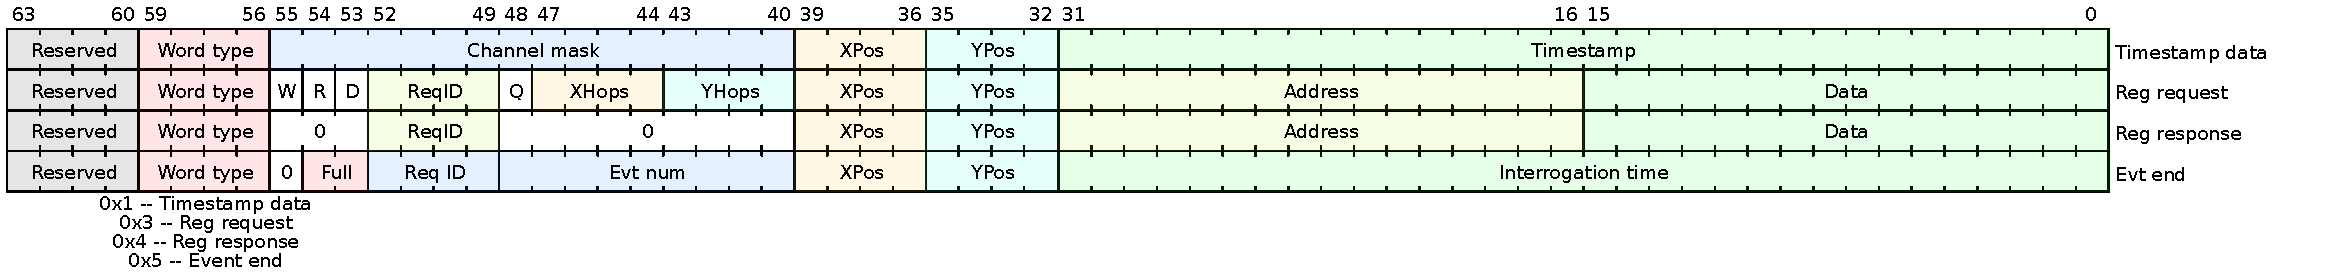
\includegraphics[width=\textwidth]{images/qpix_word_format.pdf}
\caption{Example of Datum words and their allocation as currently implemented in the simulation and first prototypes.}
\end{figure}~\label{fig:datum}

\subsection{Communication of the Datum}~\label{sec:comms}

There exist many asynchronous protocols of communication of digital information.
Most of the differences between protocols exist based on the number of connections between devices and whether or not one pin is allocated to share a clock, etc.

Our design considerations for this readout include reduction of SPF risk, low power, and minimal routing.
Partly for these reasons, the design choice for communication relies on only two connections between ASICs.
One connection is defined as a data receiver (Rx) and the other as a data transmitter (Tx).
This choice of interface dramatically limits a choice of possible protocols.
Here, we describe the difference between two that we tested: Universal Asynchronous Receiver-Transmitter (UART) and Endeavor.
We discuss and test only these two protocols for simplicity, and find it instructive to compare a proven and custom protocol (Endeavor) with a very common one (UART).

The importance of choosing a correct protocol is to ensure lossless data transmission.
Since there are free running clocks, an asynchronous communication protocol is required.
The way to ensure that data can be moved between clocks of different speeds is to stretch the signal or to repeat bits.
The more the word is stretched in time, the larger the allowable difference in frequency between the two devices.
However, this lengthening can't proceed forever, obviously, otherwise data transmission time could exceed data capture rates.

It is another important design consideration, then, to ensure that transactions proceed as quickly as possibly without data loss.
Additional concerns of long data transactions include the use of more clock cycles which use more power and increase the risk noise to leak to the analog front-end.

%% appendix??
\subsubsection{UART}~\label{sec:uart}
This common protocol is typically stable between devices with a maximum difference of clock frequency to be 10\%.

\begin{tikztimingtable}[%
    timing/dslope=0.1,
    timing/.style={x=5ex,y=2ex},
    x=5ex,
    timing/rowdist=3ex,
    timing/name/.style={font=\sffamily\scriptsize}
]
\centering
% \busref{$CLK_{base-tx}$} & 0.10L 156{.1428570c} \\
% \busref{$CLK_{base-rx}$} & 0.35L 156{0.12857c} \\
\busref{$CLK_{tx}$} & 0.10L 18{c} \\
\busref{$CLK_{rx}$} & 0.35L 20{0.9c} \\
\busref*{Tx} & 0.10L 2u 1D{START} 10d{DATA} 1D{STOP} 2U \\
\busref*{Rx} & 0.35L 1.80u 0.9D{START} 10.8d{DATA} 0.9D{STOP} 1.8U \\
\extracode
\begin{pgfonlayer}{background}
\begin{scope}[semitransparent ,thick]
\vertlines[darkgray,dotted]{0.10,1.10,...,2.1}
\vertlines[black,solid]{0.35,1.25,...,10.25}
\end{scope}
\end{pgfonlayer}
\end{tikztimingtable}~\label{tikz:uart}

%% appendix??
\subsubsection{Endeavor}~\label{sec:endeavor}

This protocol is slower than UART, but allows for approximately double the frequency difference: $\approx$ 20\%.

The endeavor protocol relies on repeating the value of a high-bit, (digital '1' value) for an integer number of clock cycles.
The receiver continually samples in incoming data transmission and counts the number of clock cycles that the signal was high for.
The longer the signal was high, the more likely it is the the transmitter was attempting to encode a high bit, and vice verse.

The number of clock cycles which accompany either a high bit transmission or a low bit transmission then represent a possible design choice for the protocol.
The actual number of bits which should be used ultimately depend on the similarity of the frequency between adjacent digital channels; the more similar the frequency (and relative phase) the lower these numbers can be.

\begin{itemize}
    \item Start Bit
    \item High Bit
    \item Low Bit Send
    \item Stop Bit Send
\end{itemize}\label{item:endeavor}

%% This section should reference how Q-Pix fits into a DUNE APA as a design goal
\section{Constraining the Digital-Backend Design}

Section~\ref{sec:qpix_apa} describes in detail how a Q-Pix based hardware readout architecture could fit within a single DUNE-APA.
Here we extend this discussion and use those constraints as the starting point for a search for a solution to the digital back-end architecture.
The first problem to solve is how to aggregate the all timestamp data supplied by the large number of channels within a DUNE-FD APA.

A Q-Pix architecture would likely use either a high-performance FPGA or a custom ASIC to aggregate the large number of $(\mathcal{O}(10^{7})$ channels.
The number of aggregated digital channels determines the required capabilities of the aggregator node and the selection of an FPGA or ASIC.
Since each additional aggregator node represents an additional SPF risk, our design goal suggests that the optimal configuration is one that produces the least number of aggregator nodes.
Therefore, the goal is to design a routing architecture which is responsible for as many digital channels as possible for each data aggregator node which still allows for accurate timing calibration and lossless data acquisition.

However, as one increases the number of digital channels per aggregator node one also increases the amount of local oscillators per aggregator, each of which must be calibrated.
Additionally, since each digital channel requires extra communication time (as discussed in section~\ref{sec:comms}) the introduction of more channels negatively affects the precision of timing calibrations and potentially increases SPF risk of digital channels.
We consider then that an optimal number of digital channels per aggregator node is one that maximizes the number of digital channels but still maintains the required timing calibration~(Sec.~\ref{sec:background}) and transmits lossless data.

We refer to the total number of digital channels collected from one pathway to an aggregator as a tile.
In a fully realized design an aggregator might in fact be responsible for multiple tiles, which need not necessarily be the same size.
The requirements of an aggregator node is completely determined by the composition of tiles it is connected to.
Then, a parameteriziation of the data requirements imposed by each tile can be extended to describe the requirements of the aggregator node.
Finally, we reach the conclusion that the required parameterization of the back-end system relies on the parameterization of the tile.

A tile is composed of inter-connections between digital channels.
The LArTPC design suggests that each digital channel have a maximum of four connections since the collection of charge happens on a flat two-dimmensional anode plane.
Therefore, a two-dimensional routing requires at least two independent communication channels, which if we require the digital channels to allow bi-directional communication, the minimum number of channels is four.
We use this number as a starting point for the digital channel design.
These four connections per channel immediately creates a rectangular connection structure for a tile.

% once aggregator is selected, hardware can be parameterized
We note here that in order to meet other physical design requirements to fit into a pre-existing APA frame, the capability of the aggregator nodes could be increased to be responsible for more tiles, which would reduce the cable and hardware engineering considerations.
However, further consideration here is beyond the scope of this work.

% tile connection methods
\subsection{Tile Routing Considerations}

A tile is a rectangular composition of digital channels which must provide a path to all digital channels and send lossless data to the aggregator.
Since there is one connection between a tile and the aggregator, there is one special node within the tile that connects to the aggregator.
This special node we refer to as the ``base-node'' as all data and instruction commands, regardless of routing, must pass through this node.
The symmetry of the rectangular tile allows any corner node to be the base node, and we choose the upper-left to define a convention.
An example of a tile with a Corner base-node is shown in Figure.~\ref{fig:cbn}.

We do not consider possible configurations where an aggregator might be connected to a digital channel within a tile since we require that all digtal channels are identical and fully connected.
We require identical channels as a practical choice due the required number of total channels.
We also require the tile to be fully connected to allow as many possible unique paths between the base-node and the other nodes which provides maximum protection against SPF.
We address that we discuss why we do not consider base-nodes placed on the outter edge of a tile, but not at the corners more generally in section~\ref{sec:base_node}.
Briefly, base-nodes which are along the outter edge of a FCT but not at the corners simply contain two sub-graphs of FCT with a base-node along the edge.
Therefore, an analysis of the constraints of a FCT with corner base-nodes can be mapped to an analysis of FCT with edge base-nodes.

\begin{figure}[]
\centering
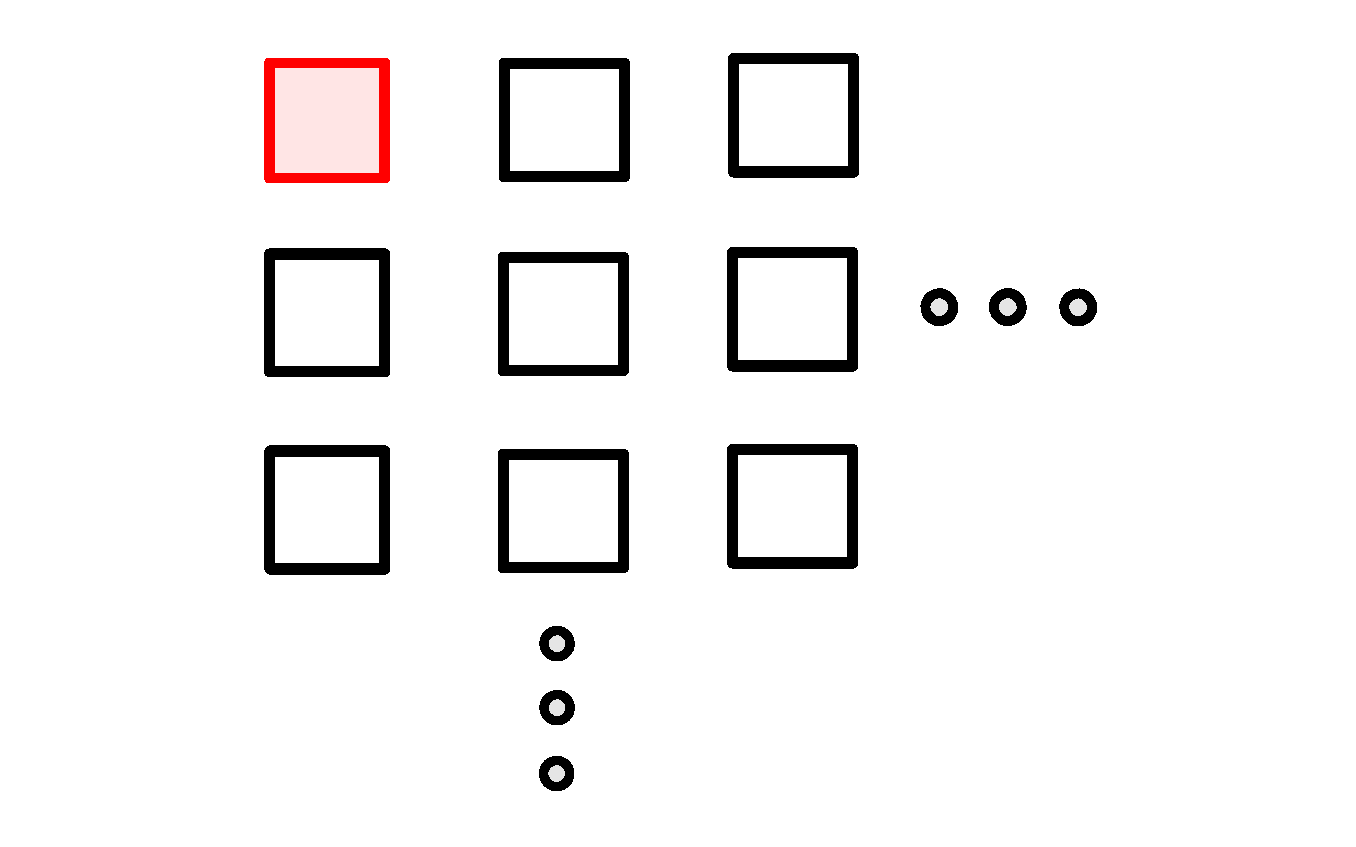
\includegraphics[width=\textwidth]{images/CBN.pdf}
\caption{Example of an Corner base-node configuration. The base-node is colored and highlighted in red.}
\end{figure}~\label{fig:cbn}


Here we introduce a particular representation (based on graph-theory) for a tile which is useful for simplifying simulations and for analyzing particular routing configurations.
The most general tile configuration occurs when we assume that all adjacent nodes within the tile are connected; this creates what we refer to as a ``fully connected tile'' (FCT).
An example of a FCT is shown in Figure~\ref{fc_tile}.
Any particular choice of an effective routing must then be a subset of this fully connected version.

\begin{figure}[]
\centering
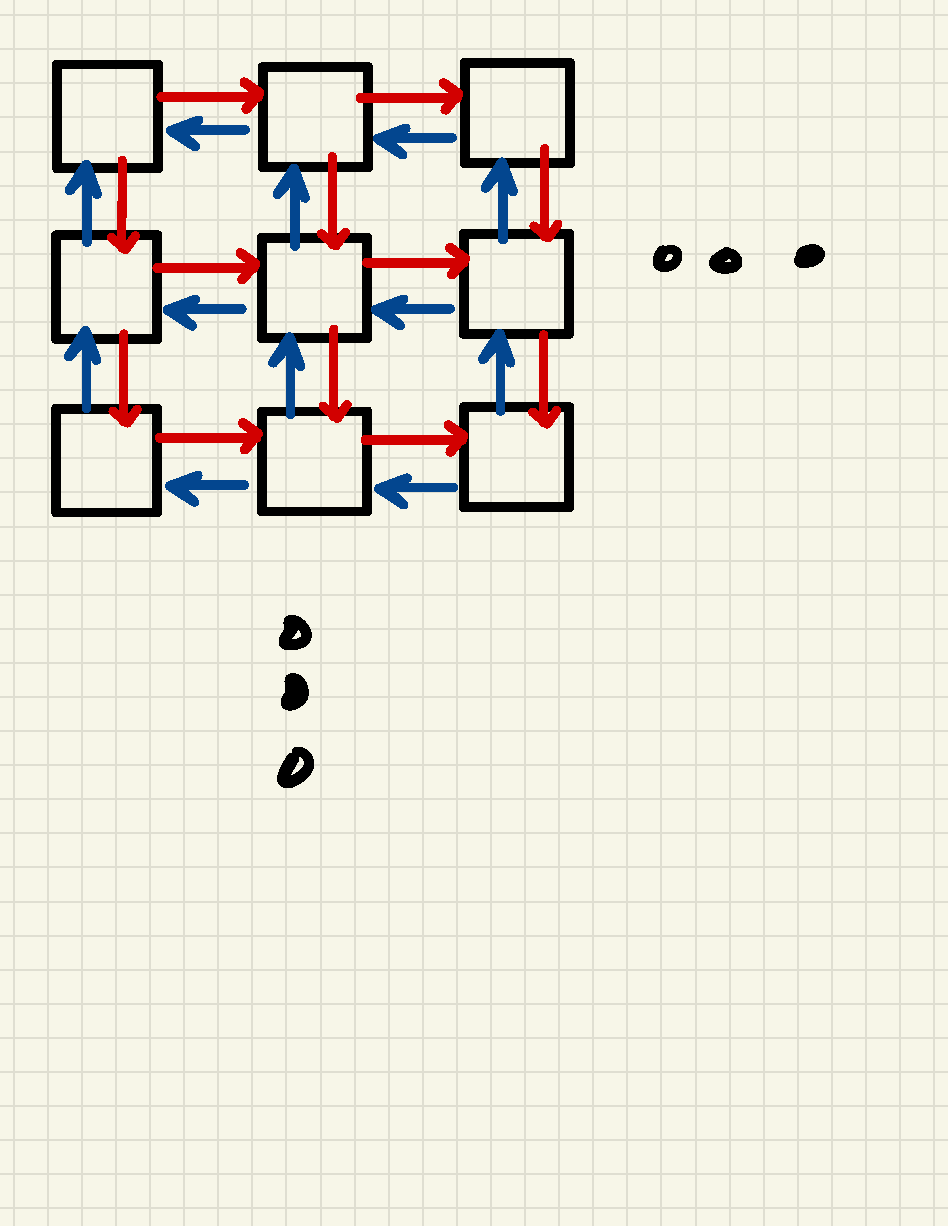
\includegraphics[width=\textwidth]{images/Notes.pdf}
\caption{Example of the fully connected routing configuration for a tile (FCT). Each Node represents a digital channel which must be aggregated, and the red and blue connections distinguish directions of communication. The red connection lines indicate pathways away from the base node, whereas the blue lines represent connection paths towards the base-node in the upper-left.}
\end{figure}~\label{fig:fc_tile}

To elaborate on the adjacency matrix of the FCT we consider an $2\times 3$ tile.
A $2\times 3$ tile has six total nodes, where we consider the upper-left most node to be the base node.
Then, the unweighted adjacency matrix has dimensions $6\times6$ of the form:
\begin{equation}
M =
 \begin{pmatrix}
 0 & 1 & 0 & 1 & 0 & 0 \\
 1 & 0 & 1 & 0 & 1 & 0 \\
 0 & 1 & 0 & 0 & 0 & 1 \\
 1 & 0 & 0 & 0 & 1 & 0 \\
 0 & 1 & 0 & 1 & 0 & 1 \\
 0 & 0 & 1 & 0 & 1 & 0 \\
 \end{pmatrix}
\end{equation}~\label{eq:adjacency_matr}

Where each non-zero value of $M_{ij}$ represents a connection between nodes $i$ and $j$.
As an unweighted, undirected graph this is a symmetric matrix.

In practice each digital channel within a tile is actually controlled by a unique, free-running oscillator.
Therefore, we can define the length of each edge between nodes as the length of time to send of a packet of data between two nodes ($T_{i\rightarrow j}$).
With this we can extend the model the adjacency matrix as a weighted and directed graph if we recognize that the non-zero elements of $M_{ij}$ become $T_{i\rightarrow j}$, or the length of time it takes for the $i^{th}$ local oscillator to transmit a packet to node $j$.

We can generalize this matrix in terms of an arbitrary number of rows ($r$) and columns ($c$).
We define a convention of numbering nodes within the tile in terms of increasing column number followed by increasing row number.
With this convention we obtain the general adjacency matrix with values defined by:
\begin{equation}
  M_{ij} = T_{i\rightarrow j}(\delta_{i,j=i\pm 1} + \delta_{i,j=i\pm r})
\end{equation}~\label{eq:adjacency_comp}

An adjacency list can similarly be constructed from Equation~\ref{eq:adjacency_comp} where the non-zero connections are given by the kroniker-deltas.

The length between the nodes represets the time it takes for a packet to transact from one node to the next.
This is determined by both the number of bits to be sent in the communication protocol ($N_{bits}$) and the frequency of the local oscillator ($f_{i}$).
We note that the receiving local oscillator also affects the true transaction time up to a single clock cycle.
However, since the transaction time of a packet is much larger than a single clock cycle ($N_{bits} \simeq \mathcal{O}(10^{2}) \gg 1$), we can approximate:

\begin{equation}
T_{i\rightarrow j} \approx T_{i} = N_{bits}/f_{i}
\end{equation}~\label{eq:t_packet}

This representation is also useful to model certain SPF where a node becomes inactive.
Dead or inactive nodes are ones in which all of their connections are effectively disconnected.
This is equivalent to setting their transaction lengths to zero: $T_{SPF} = 0$.

We comment that although it is possible to construct tiles where more than one node connects to the aggregator, we observe that this configuration simply produces two effective tiles.
These distinct tiles then are the data paths which are unique to each base-node.
In this graphical representation a packet of data can follow one, and only one path from the origin node to the base-node unless there was duplication of packets.
We emphatically avoid designs which might depend on data duplication for reduncancy; these two base-nodes are in unconnected graphs.

Additionally, it is possible to connect non-rectangular tiles, but these tiles are effectively a larger rectangular tile with disconnected nodes to produce the desired shape.
Since every node is designed to be robust in the full version, it will be be robust in the subset.

We can apply this same argument to base-nodes which do not lie at the corners of the rectangular tile.
In the case where the base-node is selected along the edge
Therefore, we conclude that the analysis of the tile with the above adjacency matrix and a selection of the base-node at the corner of a rectangular corner provides the basis problem to the tile configuration.

\subsubsection{The SPF Cost}~\label{sec:spf_cost}

We define the average SPF cost as the amount of nodes that will be lost during a transaction as the number of digital channels at a height below the failed digital channel.
For example, the number of nodes which are lost if a leaf-node fails is one since no other channels are between it and the data node.
Likewise, the number of nodes which are lost in the event of a base-node failure is the total tile, $N$.

We can then calculate a mean cost SPF, $C_{SPF}$, :

\begin{equation}
  C_{SPF} = \frac{1}{N}\sum_{node} \frac{n_{i}}{N} = \frac{1}{N^{2}}\sum_{node} n_{i}
\end{equation}~\label{eq:cspf}

\subsubsection{Minimize Occupancy}~\label{sec:min_conn}

One of the goals of a succesful digital design is to ensure lossless data transfer.
One point of failure on the digital side is an overabudance of data arriving at a single layer within the tree.
This data loss occurs when data are sent to a node faster than the data leaves the node, and persists for long enough such that the buffers of the node overflow.
This creates a horrible loss of data which can't be recovered.

A routing scheme which minimizes the overall occupancy in the tree depths is shown in Figure~\ref{fig:snake}.
We refer to the style of routing as ``Snake''-routing (SR), because this is also the longest possible routing scheme for a square tile.

\begin{figure}[]
\centering
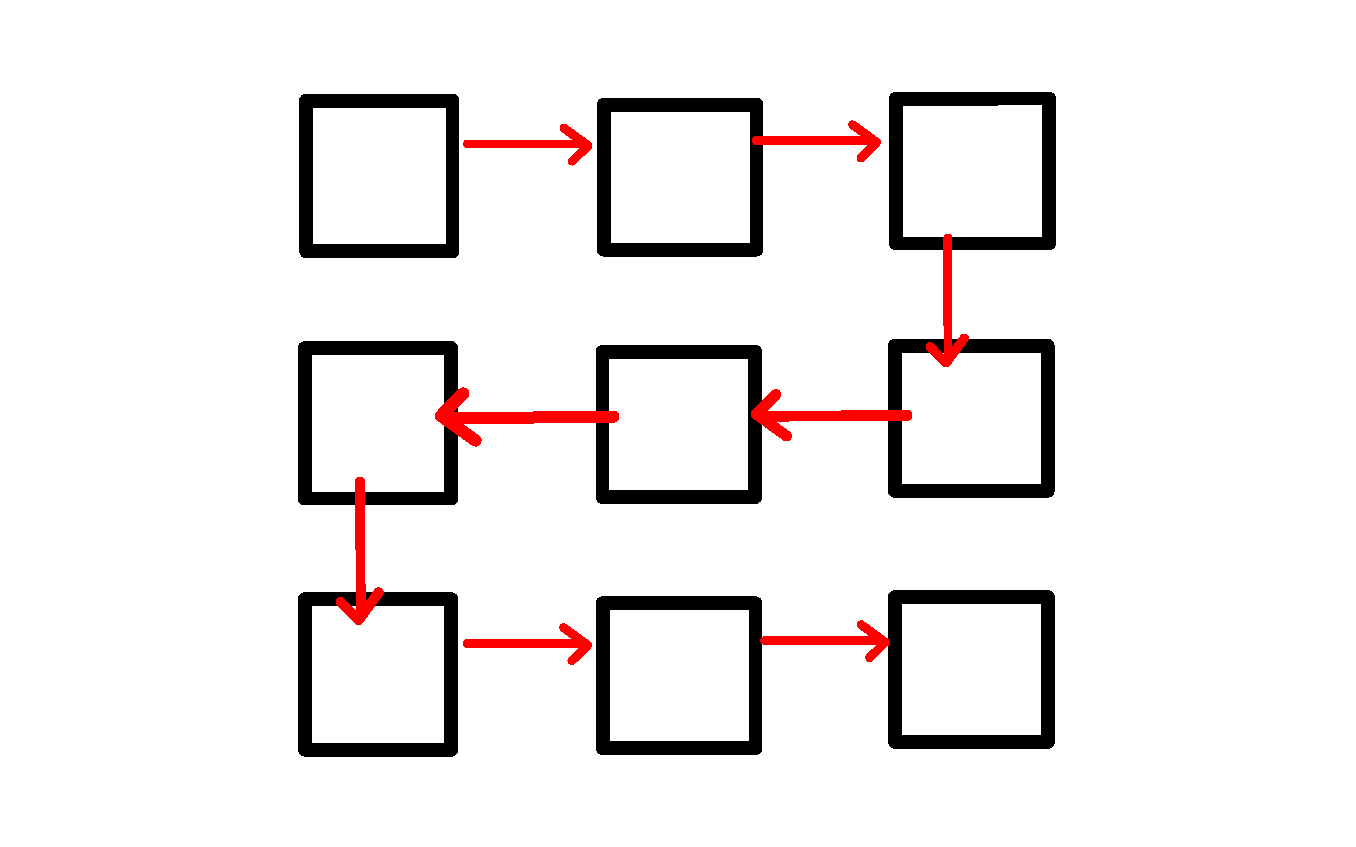
\includegraphics[width=\textwidth]{images/snakeroute.pdf}
\caption{Minimal Occupancy Path of a FCT. This routing path ensures that the number of input connections equal the number of output paths for the node.}
\end{figure}~\label{fig:snake}

We inspect the SPF risk from this routing scheme with Equation~\ref{eq:cspf}, where we notice that the $n_{i}$ of each node is simply a running sum from the leaf to $N$ at the base node.

\begin{equation}
  C_{SPF} = \frac{1}{N^{2}}\frac{N(N+1)}{2} = \frac{1}{n}\frac{N+1}{2} = \frac{1}{2} + \frac{1}{2N}
\end{equation}~\label{eq:cspf_snake}

Equation~\ref{eq:cspf_snake} tells us that the SPF risk of this routing configuration converges to half as the size of the tile grows.
Intuitively, this makes sense, since it is equally likely to select a node close to the base-node as it is far away, which implies that the sum should converge to half the tile size for large $N$.

Although this routing scheme provides the most lax constraint on the requried buffers at each digital channel, it provides the longest average path between the base node.
The longer the transaction delay between the base-node and other nodes increases the reconstruction time uncertainty.
Therefore, a natural alternative routing scheme is one that minimizes the communication scheme.

\subsubsection{Minimize Delay}~\label{sec:min_comm}

For any given node in an edge FCT with location $(R_{i},C_{i}$), the shortest path to the base-node is simply the sum of its coordinates: $R_{i}+C_{i}$.
An example of such a routing configuration for a tile is shown in Figure~\ref{fig:leftroute}.

\begin{figure}[]
\centering
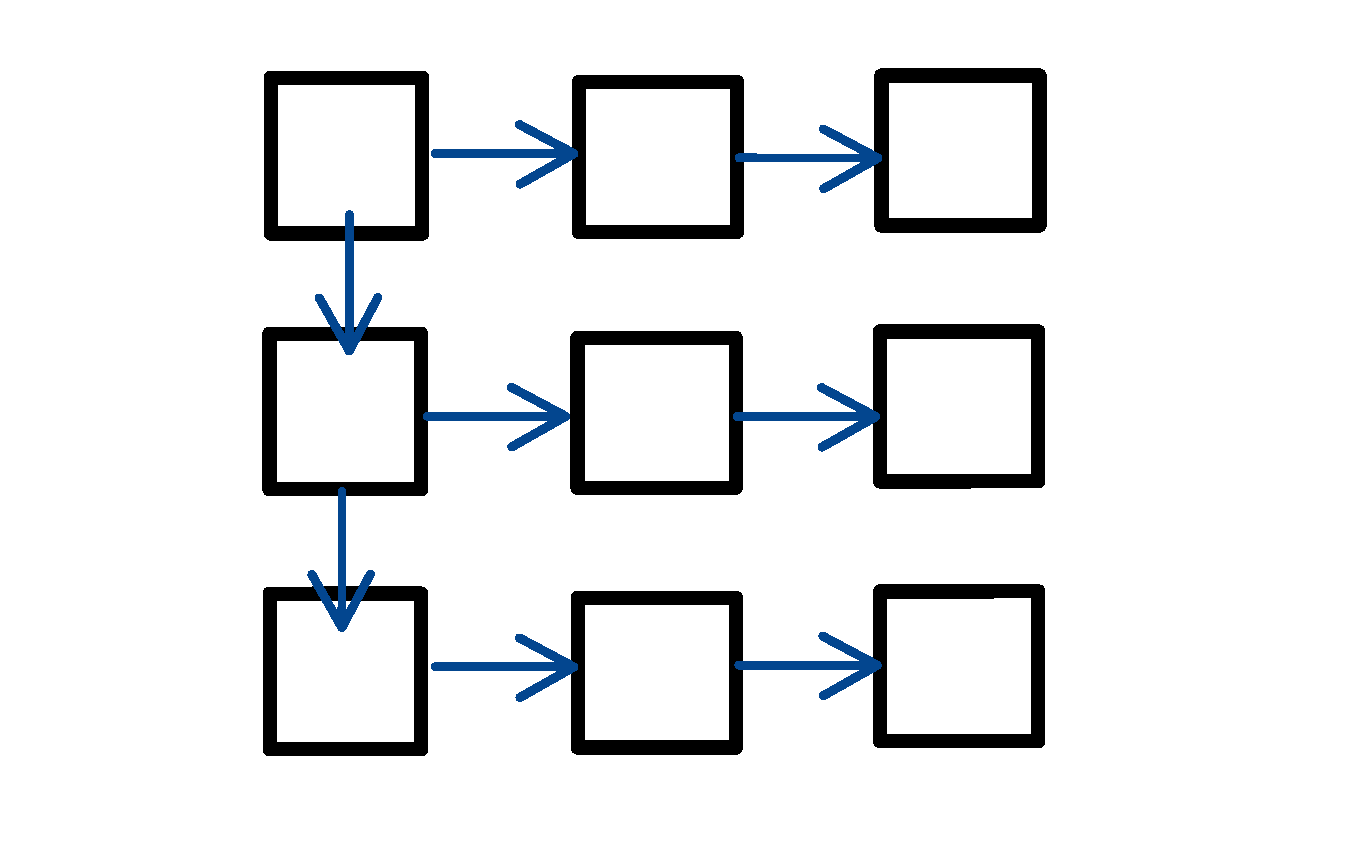
\includegraphics[width=\textwidth]{images/leftroute.pdf}
\caption{Minimal Delay Path of a FCT. This routing path ensures that the minimum number of transactions occur from every node in the FCT to reach the base-node. For any node along any column this is equivalent to the sum of the row and column of that node.}
\end{figure}~\label{fig:leftroute}

We can calculate $C_{SPF}$ for this routing configuration if we identify that there are a $C$ number of rows which sum from one to $R-1$.
Likelise, the far-left column in Figure~\ref{fig:leftroute} shows that the number of rows, $R$, sum from one to $C$.
We can rewrite the sum over all nodes in Equation~\ref{eq:cspf} as:

\begin{equation}
  \sum_{node}n_{i} = C\sum_{i=0}^{i=R-1}i + R\sum_{i=0}^{i=C}i
\end{equation}~\label{eq:cspf_left_s}

We simplify the running sum of each term in Equation~\ref{eq:cspf_left_s}:
\begin{equation}
  \sum_{node}n_{i} = C\frac{R(R-1)}{2} + R\frac{C(C+1)}{2} = RC(\frac{R+C}{2})
\end{equation}~\label{eq:cspf_left_e}

Using this result we obtain $C_{SPF}$ by identifying $N = RC$:
\begin{equation}
  C_{SPF} = \frac{1}{N^{2}}\sum_{node}n_{i} = \boxed{\frac{R+C}{2RC}}
\end{equation}~\label{eq:cspf_left_fin}

This result informs that relative cost of losing a node tends to zero as the size of the tile grows.
Again, this result can be obtained intuitively, since as the number of columns (or rows) grow in size, the probability of a single failure occuring on the aggregator column is increasingly less likely.


\subsubsection{Broadcasts to avoid SPF}~\label{sec:broadcast}

In order to protect against SPF we only consider a designs which implement the FCT, since SPF can occur on any node the most robust connection scheme is the FCT.
A FCT allows searches to probe all possible paths to any node via a ``broadcast'' produced from packets sent by the aggregator to the base-node.
Therefore the broadcast algorithm can be represented by a complete circuit which begins at the base-node and proceeds to a target node with no repeated nodes until the target node is reached.
The backward path is then completed in reverse by following the edges (connections) between each node until arriving finally again at the base-node.

In practice, we encode the broadcast packet with a special header, to separate it from a request packet, and include an identification number.
Then, any node which receives a broadcast packet will record the identification number of the most recent broadcast, which it can use to discard additional broadcast packets that arrive with the same number.

In the event that a particular node becomes inactive it will ``block'' data comming from the nodes along its path.
In this case, there must be some sort of ``broadcast'' originating from the base-node that would allow information tranverse regardless of the effective routing path.


\begin{figure}[]
\centering
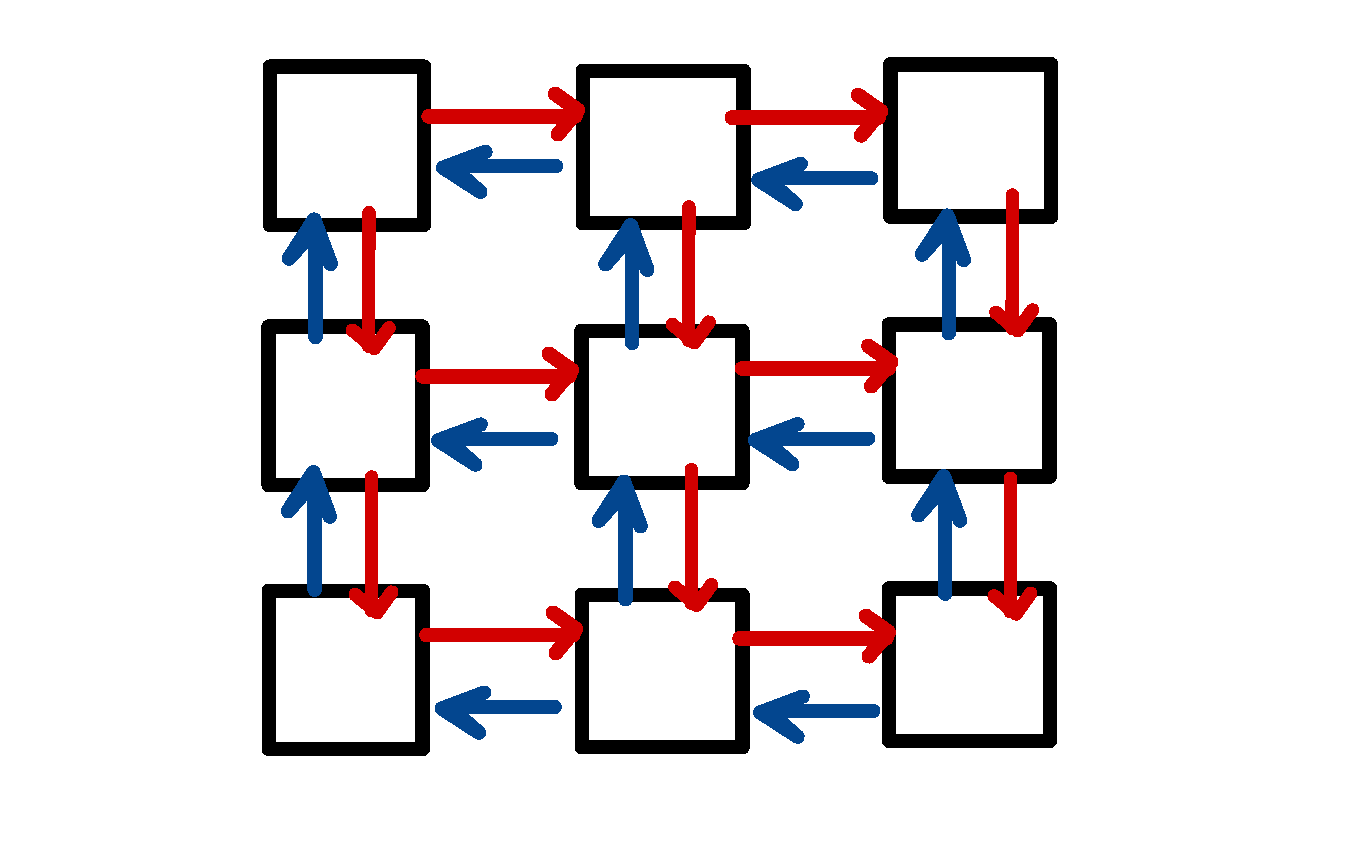
\includegraphics[width=\textwidth]{images/Broadcast.pdf}
\caption{Minimal Routing Path of a FCT. This routing path ensures that the number of input connections equal the number of output paths for the node.}
\end{figure}~\label{fig:broadcast}

\subsection{Comments on the Edge Base-node and Other Routings}~\label{sec:base_node}

We discuss here the case of a FCT with an edge base node.
An edge base node (EBN) is a digital channel that connects to the aggregator and to three other digital channels within a tile.
Like before, this base-node must provide a unique path during data transmission to all digital channels within the tile.
In this configuration the adjacency matrix is still the same as given in Equation~\ref{eq:adjacency_comp}.

Also, as before, we wish to inspect different routing scenarios for a tile of a given square dimension of $R$ rows and $C$ columns.
We can proceed by dividing the FCT graph into two subgraphs, $S1$ and $S2$, where $S1$ represets the rectangular section of the graph below and to the left of the EBN, while $S2$ are the remaining channels.

We identify that while the number of columns ($C$) in tile is equal to both subgraphs, the total number of rows $R$ of the tile is equal to the sum of the rows from these two subgraphs: $R = R_{1} + R_{2}$.

\begin{figure}[]
\centering
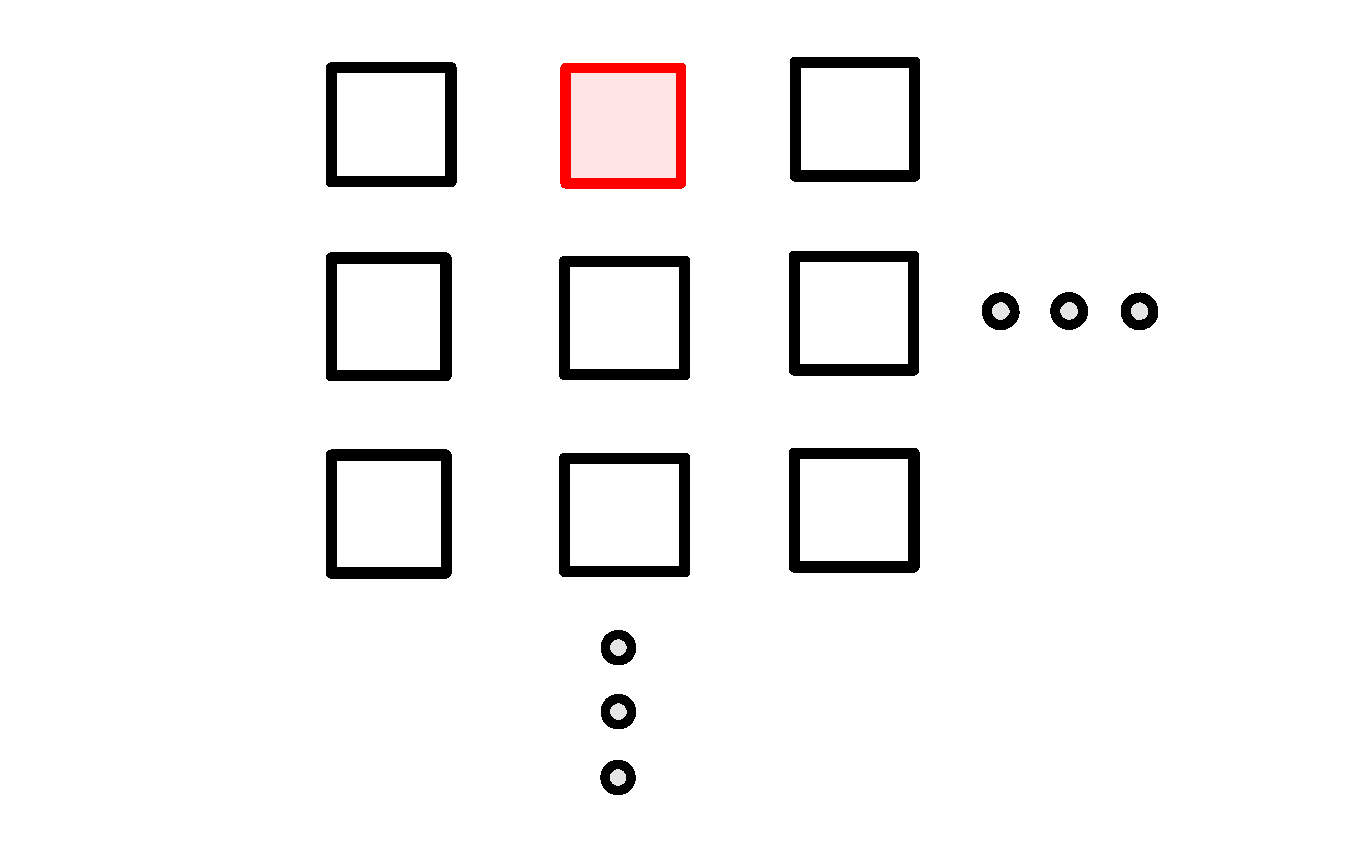
\includegraphics[width=\textwidth]{images/EBN.pdf}
\caption{Example of an Edge base-node configuration. The base-node is colored and highlighted in red.}
\end{figure}~\label{fig:ebn}

\begin{tikzpicture}[->,>=stealth',shorten >=1pt,auto,node distance=1.25cm,
                    ,auto=center]
                    % ,auto=center,every node/.style={circle,fill=blue!20}]
  \tikzstyle{every node}=[fill=blue,draw=none,text=white]

  \node (1) at (0,0) {1};
  %% row 1
  \node (2) at (1,-1) {2};
  \node (3) at (2,-2) {3};
  \node (4) at (3,-3) {4};
  % row 2
  \node (5) at (0, -1) {5};
  \node (6) at (1,-2) {6};
  \node (7) at (2,-3) {7};
  \node (8) at (3,-4) {8};

  %% end nodes
  \node (10) at (0, -5) {$C$}; % must be at 0 x
  \node (11) at (5, -5) {$R$}; % must be 1:1 slope
  \node (12) at (5, -10) {$R+C$}; % must be 1:1 slope

  %% paths
  % \path (4) -- (11) [red, midway, sloped] {$\dots$};
  % \path (5) -- (10) [red, midway, sloped] {$\dots$};
  \draw[red,thick,dashed] (4) -- (11);
  \draw[red,thick,dashed] (5) -- (10);
  \draw[red,thick,dashed] (10) -- (12);
  \draw[red,thick,dashed] (11) -- (12);

  \path (1) edge (2);
  \path (1) edge (5);
  \path (2) edge (3);
  \path (3) edge (4);
  \path (5) edge (6);
  \path (6) edge (7);
  \path (7) edge (8);
\end{tikzpicture}

The EBN then is actually just a composition of two subgraphs which are each equivalent to
The tree characteristics which determine requirements for the digital channels are the tree height and total occupancy at each level.
Therefore, since the EBN provides no difference in either of these characteristics and is a suposition of two fundamental CBN, an analysis of an EBN is equivalent to the analysis of a CBN.

However, we do remark comment that the average difference of the relative weights of each node in a SPF analysis are different in a EBN compared to the CBN case.
This should be obvious since the relative weight of each node is determined by the running sum of the path length betwee the base-node and its leaf.
For a fixed row dimension, $R$, the EBN offers a smaller average tree height for each of its componet radia $R_{1}$ and $R_{2}$.

Therefore, in a EBN tile, with two subgraphs of radii $R_{1}$ and $R_{2}$ where the base-node is on the $R_{1}$ edge.
The total sum of the weights of all nodes in the tile are the sums of the two subgraphs plus $CR_{2}$, which is the average weight of the nodes from the subgraph $R_{2}$ when it connects to $R_{1}$.
\begin{equation}
  \sum_{node}n_{i} = \sum_{R_{1}} + \sum_{R_{2}} + CR_{2}
\end{equation}~\label{eq:cspf_ebn}

Equation~\ref{eq:cspf_ebn} gives the general formula for calculating the SPF risk for a EBN case, depending on the routing methods of subgraphs $R_{1}$ and $R_{2}$.
We can treat these sub-graphs as in equation~\ref{eq:cspf_left_fin} to obtain:
\begin{equation}
  \sum_{R_{1}} + \sum_{R_{2}} + CR_{2} = \frac{R_{1}C(R_{1}+C)}{2} + \frac{R_{2}C(R_{2}+C)}{2} + CR_{2}
\end{equation}~\label{eq:cspf_e}

We use this result to obtain the relation of the general $C_{SPF}$:
\begin{equation}
  C_{SPF} = \frac{1}{N^{2}}(\frac{R_{1}C(R_{1}+C)}{2} + \frac{R_{2}C(R_{2}+C)}{2} + CR_{2})
\end{equation}

if we identify that $N = C(R_{1}+R_{2})$ and use $R_{2} = R - R_{1}$:
\begin{equation}
  C_{SPF} = \frac{1}{2CR^{2}}(2R_{1}^{2}-2R_{1}R+R^{2}+CR+2(R-R_{1}))
\end{equation}


\section{Frequency Calibration of Local Oscillators}~\label{sec:calib}

The Q-Pix calibration requirements are described in detail in Section~\ref{sec:qpix_calib}.
The important parameters which must be calibrated for each pixel are the charge per reset and the frequency of the local oscillator.
An aim of this work is to demonstrate an additional frequency calibration method using the minimal required connections between each digital node.

Any method of a frequency calibration must synchronize time measurements between all digital nodes within a tile and the aggregator.
There are several possibile methods to achieve this, but ultimately the data that are recorded must be some time at the aggregator, $T_{a}$, and the time at any specific node, $T_{j}$.

%% distribute clock for calibration of time
A direct method is one where the aggregator distributes its own clock to all nodes in the tile.
This scenario removes the need for a calculation of the frequency of each node altogether since the clock of each node is already known from the aggregator.
This is the simplest case for timing calibration: remove all free running oscillators.
However, this method also introduces complex routing and power requirements within every tile.

A distributed clock network indeed removes ambiguity of the remote oscillator frequencies, but at the cost of hardware complexity.
Whether or not this design choice is preferred is entirely detector dependent.

We comment, however, that we ignore this scenario because it may altogether be unnecessary depending on future ASIC performance.
In the event that frequency calibrations of sufficient precision ($\bar{f} \approx 1 ppm$) are possible occur on free-running local oscillators future detectors would need only to acquire these ASICs and place them with minimal cost in terms of both time and money.

%% distribute trigger for calibration of time
Another simple scenario is one where the aggregator itself connects directly to all nodes within a tile via a single connection which can be used as a reference trigger.
This means that some trigger from the aggregator would issue directly into each node at the same time: $T_{a} = T_{n}$.
To calcuate the frequency in this manner, the controller would issue two triggers from the aggregator with a known time separation, $T_{o} = T_{a2} - T_{a1}$.
The remote nodes would each record and send their timestamps back to the aggregator, where the time difference would be calculated as:

\begin{equation}
  T_{o} = T_{a2} - T_{a1} = T_{n2} - T_{n1}
\end{equation}

this is rewritten in terms of frequency as follows:
\begin{equation}
  f_{n} = \frac{T_{n2} - T_{n1}}{T_{o}}
\end{equation}

This calibration method extremely simple but introduces an additional connection to each node between itself and the aggregator.
For a large scale system such as Q-Pix even this simple connection scheme introduces $\approx 60k$ hardware points of failure per APA.

Both of these scenarios are valid implementations of a Q-Pix readout system.
In both of these scenarios, however, there is added complexity into the hardware design of the system in the form of additional routing where each route which represents a possible point of failure.

In a world of perfect hardware and costless routing in terms of both time and money these routing schemes would clearly be sufficient.
However, no hardware is perfect.
Therefore we introduce and discuss a calibration technique which relies on no additional routing and could be optionally implemented even in the above schemes in the event of a failure.
Therefore, even if not the primary implemented calibration technqiue, since this calibration introduces no superfluous routing it could still be used regardless of the actual future hardware implementation.

%% distribute packet for calibration of time
\subsection{A Minimal Connection Calibration Procedure}~\label{sec:min_calib}

As stated in the previous section, any frequency calibration records a reference time at the aggregator ($T_{a}$) and an event time ($T_{n}$) at a node within a tile.

This time calibration procedure requires only the communication pathways in the system, where we assume time-dependent free-running local oscillators at each node within the tile.

%% issue 1
The calibration procedure begins at a time ($T_{0}$) where the aggregator sends a calibration packet.

%% recv1
Next, the packet propagates through the tile to some remote node, $N_{j}$.
This node receives the packet later at some time $T_{n1}$:

\begin{equation}
  T_{n1} = T_{o} + T_{f1}
\end{equation}

Where $T_{f1}$ is the propogation time through the array.

%% meas1
This remote node then sends the packet with its time ($T_{n1}$) back to the aggregator.

%% wait
The aggregator will wait some calibration time ($T_{cal}$) before issuing another calibration packet.
This wait period $(\mathcal{O}(10^{0-2})$) can be long compared to the full transaction time $(\mathcal{O}(10^{-5})$) of a packet through the entire node.

%% issue 1
After the wait period, the aggregator will issue a second calibration packet to be sent to a remote node at time:
\begin{equation}
  T_{1} = T_{cal} + T_{0}
\end{equation}

%% recv2 and meas2
Similarly to the first packet this packet will propagate forward with a new time $T_{f2}$ and backward $T_{b2}$ :
\begin{equation}
  T_{n2} = T_{1} + T_{f2}
\end{equation}

Now, we define $T_{j}$ as the difference in the two time measurements from the two packets sent from the aggregator.
In this case the time difference is related to the number of clocks that occured between the two different measured values of the clock, $T_{n1}$ and $T_{n2}$.

\begin{equation}
  \Delta T_{j} = T_{n2} - T_{n1}
\end{equation}

We use the known relationships for $T_{n2}$ and $T_{n1}$ to obtain:
\begin{equation}
  \Delta T_{j} = (T_{1} + T_{f2}) - (T_{o} + T_{f1}) = (T_{1} - T_{0}) + (T_{f2} - T_{f1}) = T_{cal} + \Delta T_{f}
\end{equation}

Where we defined $\Delta T_{f}$ as the difference in forward propagation times from the packets sent from the aggregator node at $T_{1}$ and $T_{0}$.

We arrive at the result which compares the measured time at the aggregator $T_{cal}$ and the time measured at each node, $\Delta T_{j}$:
\begin{equation}
  \Delta T_{j} = T_{cal} + \Delta T_{f}
\end{equation}

A perfect reconstruction of the nodal frequency would follow if $\Delta T_{f} = 0$.
But it is sufficient to note that the wait period happens on the order of seconds, whereas $\Delta T_{f}$ is on the order of $\mu s$ or at least a six order of magnitude difference.
We then use $\Delta T_{f} \ll T_{cal}$ to obtain:
\begin{equation}
  \Delta T_{j} \approx T_{cal}
\end{equation}

We convert time into frequency with the difference of the timestamps measured and a known aggregator frequency ($f_{a}$):
\begin{equation}
   \frac{\Delta N_{j}}{f_{j}} = \frac{\Delta N_{a}}{f_{a}}
\end{equation}

or,
\begin{equation}
   \boxed{f_{j} = \frac{\Delta N_{j}}{\Delta N_{a}}f_{a}}
\end{equation}

Where $\Delta N_{j}$ and $\Delta N_{a}$ are the differences in the timestamps of the 32-bit clocks at the remote node and aggregator, respectively.


\subsubsection{Packet Transaction Time}

 We next examine the approximation that $\Delta T_{f} \ll T_{cal}$ and consider its contribution to the error in the reconstruction of $T_{j}$.
This analysis also provides a constraint on the duration of $T_{cal}$ to ensure an accurate measurement of each $T_{j}$ in a tile.
We begin by discussing how long it takes for a packet to traverse a tile.

The time it takes for each packet to be received by the next node is given in Equation~\ref{eq:t_packet}.
The value, $N_{bit}$, is the number of clock cycles used for the packet and is protocol-dependent.
Since the protocol must be deterministic for each packet, $N_{bits}$ must be the same for each transaction on the path from the base-node to the remote node.

As an example, the time it takes for a packet to go from the base-node, $N_{1}$, to a remote node, $N_{3}$, via the path $1\rightarrow 2 \rightarrow 3$ is determined by:
%% packet transaction time
\begin{equation}
  T_{1\rightarrow 3} = T_{1\rightarrow 2} + T_{2\rightarrow 3} \approx \frac{N_{bits}}{f_{1}} + \frac{N_{bits}}{f_{2}} = N_{bits}(\frac{1}{f_{1}} + \frac{1}{f_{2}})
\end{equation}~\label{eq:t_packetTransfer}

Where, $f_{i}$, is the frequency of the clock at sending node. The approximation is within a single clock cycle of the receiving digital node ($\approx 33~\unit{ns}$).

Therefore the time it takes for a packet for go from the base-node to any remote node is proportional to $N_{bits}$ multiplied by the sum of the edges in the full adjacency matrix given by Equation~\ref{eq:adjacency_comp}.

We generalize Equation~\ref{eq:t_packetTransfer} to represent the time it takes a packet to go from the aggregator ($i = 0$) to any remote node, $N_{j}$:
\begin{equation}
  T_{f} = T_{0\rightarrow j} = N_{bits}\sum_{i=0}^{i=j-1}\frac{1}{f_{i}}
\end{equation}

We require that every calibration packet on the protocol uses the same number of clocks ($N_{bits}$ is constant) and follows the same path. $\Delta T_{f}$ becomes:
\begin{equation}
  \Delta T_{f} = N_{bits}\sum_{i=0}^{i=j-1}\frac{1}{\Delta f_{i}} = N_{bits} \sum_{i=0}^{i=j-1}\Delta T_{i}
\end{equation}

We recognize $\Delta T_{i}$ as the nominal time-dependent clock drift of the each local oscillator in the path between the base-node to the remote-node.
We can provide an order of magnitude estimate for $\Delta T_{f}$ if we assume a (very poor) $\approx 1\%$ drift in each of the remote clocks within the tile during a period of $T_{cal} \approx 1~\unit{s}$.
In this approximation we also assume that the mean of the periods of the nodes are the designed value ($\approx 33~\unit{ns}$) for which a 1\% error gives $\sigma_{T_{f}} \approx 3~\unit{ps}$.
If we assume that all of the clocks (for whatever reason) drift have error which drifts int he same direction (the sum doesn't cancel) then for 100 transactions with 200 bits per transaction, we obtain for $\Delta T_{f}$:
\begin{equation}
  \Delta T_{f} \approx 200 * 100 * 3\times 10^{-12} \approx 6~\unit{ns}
\end{equation}


%%
\section{Physical Simulation Studies}

%%
\section{Background Rates and Calibration}

sources of backgrounds are taken from \citep{DUNE-FD_TDRv4:Abi_2020}

\section{Supernova Studies}

Work has been done to understand how a Q-Pix based DUNE-FD would measure core collapse supernovae \citep{qpix:shion}.

Simulation studies which involved particle interactions were based on Geant4 \citep{geant4:AGOSTINELLI2003250}.


\section{Looking for Hadron Decay}

\section{Neutrino Beam High Energy Studies}

\section{Summary and Further Studies}


%% chapter 6 - Summary and Outlook
\chapter{Summary and Outlook}
\label{chap:summary}
\section{Conclusions}

The results presented in this work provide the first tests and verification of the digital back-end for novel readout technology targeted at liquid Argon Time-Project-Chambers.

The first Q-Pix analog prototype using Off-The-Shelf analog components has been built and is currently taking measurements.
This prototype promises to provide gaseous Argon diffusion measurements, which will likely be the first true physics measurement using a Q-Pix based readout.

We have built and verified the first digital prototype boards which have verified communication reliability to protect against potential data loss.
We developed a frequency calibration method for remote nodes to demonstrate Q-Pix's ability to have independent oscillators.
We used this prototype and verified the ability to reconstruct remote oscillator frequencies with a precision more than an order of magnitude required (0.1~\unit{ppm} < 1~\unit{ppm}).
These results are verified between two different interrogation frequencies.

We developed multiple simulations to model the detector's response to long ($1000 second$) run time exposure of radiogenic backgrounds as well as tested the ability to readout beam neutrino events at LBNF.
Our simulations show that the current FIFO local (64) and remote (128) depths of the digital ASIC prototype are too small.
We estimate that the local FIFO depth should be at least be able to record 426 unique resets in order to fully capture 99\% of neutrino events with energy up to 10~\unit{GeV}.
This result provides the first limit on the memory required for a Q-Pix ASIC, should it be used in a DUNE-FD module to measure neutrino oscillations.

To test the remote FIFO and frequency requirements we developed the first simulation to model the Q-Pix digital back-end response to physical events within a DUNE-FD APA.
We find that the distribution of the ASIC frequency needs to be $\approx 0.5\%$ in order to maintain obtain reliable remote FIFO depths with the current readout method. 
These results also indicate that the only reliable routing methodolgy is the "Snake" routing (Section~\ref{sec:}), which is independent of both tile size and digital architecture.
This routing ("Snake") provides a unitary relationship between the local and remote FIFO depth requirements.

\subsection{The Future of Q-Pix}

The Q-Pix design is a novel readout technology.
However, "novelty does not confer automatically benefit", David Nygren.
The full Q-Pix validation still awaits key results to demonstate its capabilities in a DUNE-FD module.
Namely, Q-Pix still needs to test both the analog and digital prototypes at cold liquid Argon temperatures.

The front-end requires a reliable replenishment circuit as well as low leakage current ($\approx 100~\unit{aA}$ or less to be below radiogenic backgrounds).
Also, the limitation of the timing from the replenishment circuit should be applied to the RTD results presented in this work.
The combination of the timing response of the analog front-end along with the neutrino simulation events here will allow accurate event reconstruction.
With these reconstructed events in hand analysis can proceed to estimate of Q-Pix's ability to perform neutrino oscillation measurements.

\subsection{Q-Pix's First and Second Digital Prototypes}

The work presented here can accurately be viewed both as a means to understand the Q-Pix's first digital ASIC and as a guide to the second digital design.
The key result of this work indicates that the local and remote FIFO depths of the second prototype should both be increased to at or above 426.
The reason the first prototype did not incorporate these larger buff sizes to begin with was due to fabrication limitiations of the ASIC.
If oscillator tests of the first prototype indicate that the mean drift between neighbor ASICs is reliably under 0.5\%, then the local oscillator need not be changed either.
All other underlying logic, with perhaps the exception of FWFT FIFOs, have been verified in the first digital prototype.
These tests need only be repeated on the first prototype ASIC.

Eventually the Q-Pix front and back-end ASICs will likely be combined into a single chip.
Still, the motivation provided by the results presented here for the second prototype (applied only to the digital portion) remain unchanged.

\section{Future Neutrino Oscillation Studies}

Although an analysis of the reconstruction of the events involving oscillation are slightly beyond the scope of the work presented here, we provide a brief summary of how the work presented here helps in that future analysis.
The LBNF beam flux, neutrino oscillations, and neutrino cross-sections all affect the neutrino event rate as a function of energy.
Instead of applying these factors, we tested against a uniform distribution of neutrino interaction energy.

Figure~\ref{fig:energy_deposit_vs_resets} clearly shows the relationship between the energy deposited and the number of resets collected.
To account for neutrino oscillation and appearance probability as a function of energy, we would use different weights for the different neutrino flavors as shown in Figures~\cref{fig:electron_interaction,fig:muon_interaction}.
The actual weights of to rebin the neutrino distribution depends on undetermined neutrino parameters.
However for both flavor of (anti)neutrino, the peak of the distribution is below 5~\unit{GeV}.
The analysis presented here uses a uniform distribution of energy up to 10~\unit{GeV}.

\begin{figure}[]
\centering
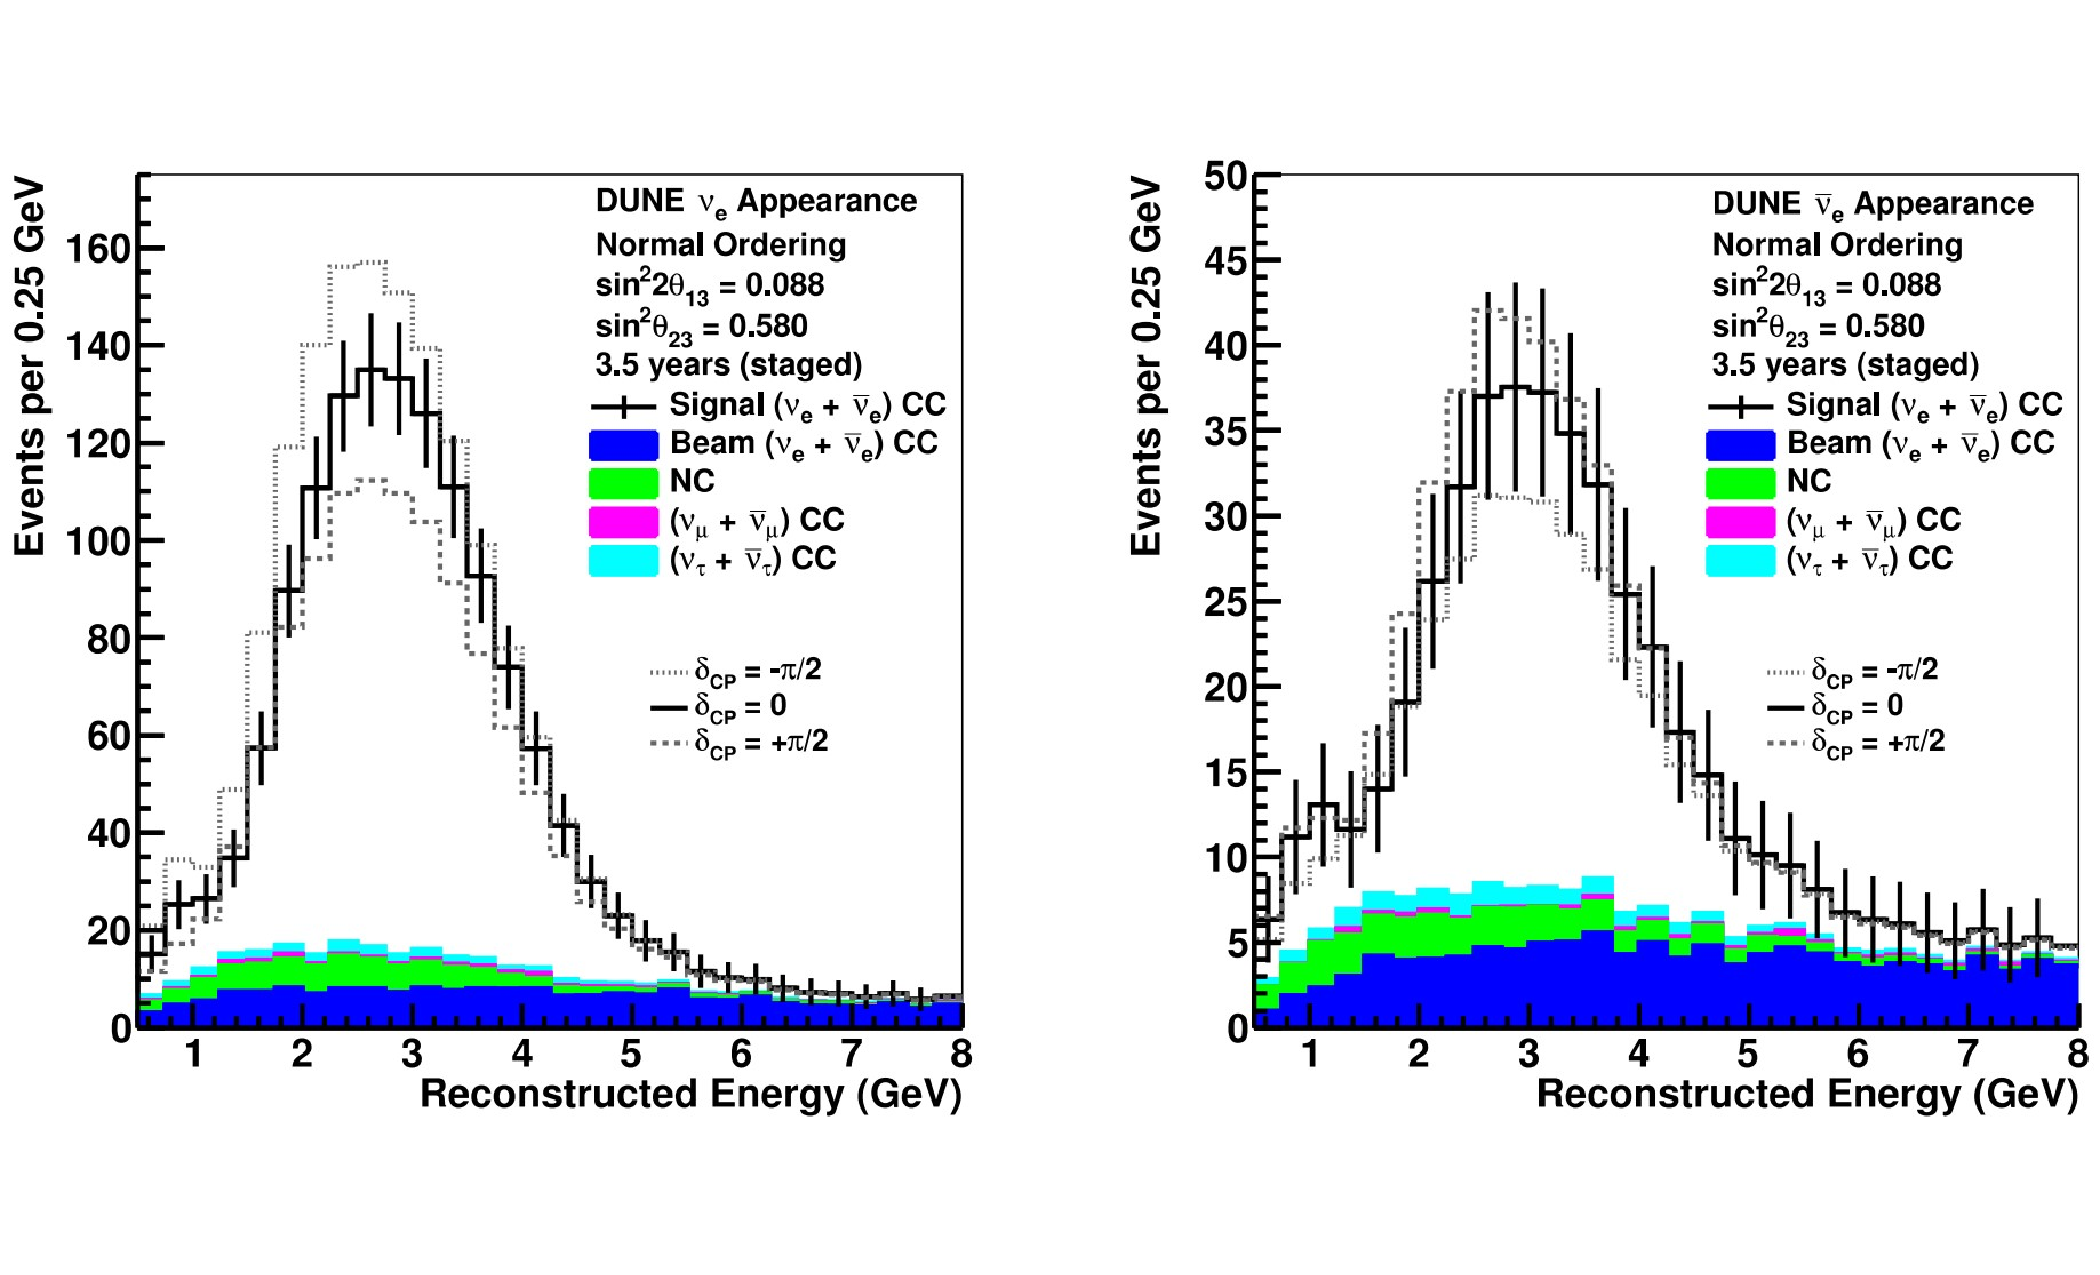
\includegraphics[width=\textwidth]{images/tdr_electron_reconstruction_tdrv2.pdf}
\caption{Figure is taken from from the DUNE-FD TDR~\citep{DUNE_FD_TDRv2_2020}.
Images show the $\nu_{e}$ and $\bar{\nu_{e}}$ appearance spectra respectively.
The left image shows the reconstructed energy distribution for the beam running in the forward horn-current direction for 3.5 years.
}
\end{figure}~\label{fig:electron_interaction}

\begin{figure}[]
\centering
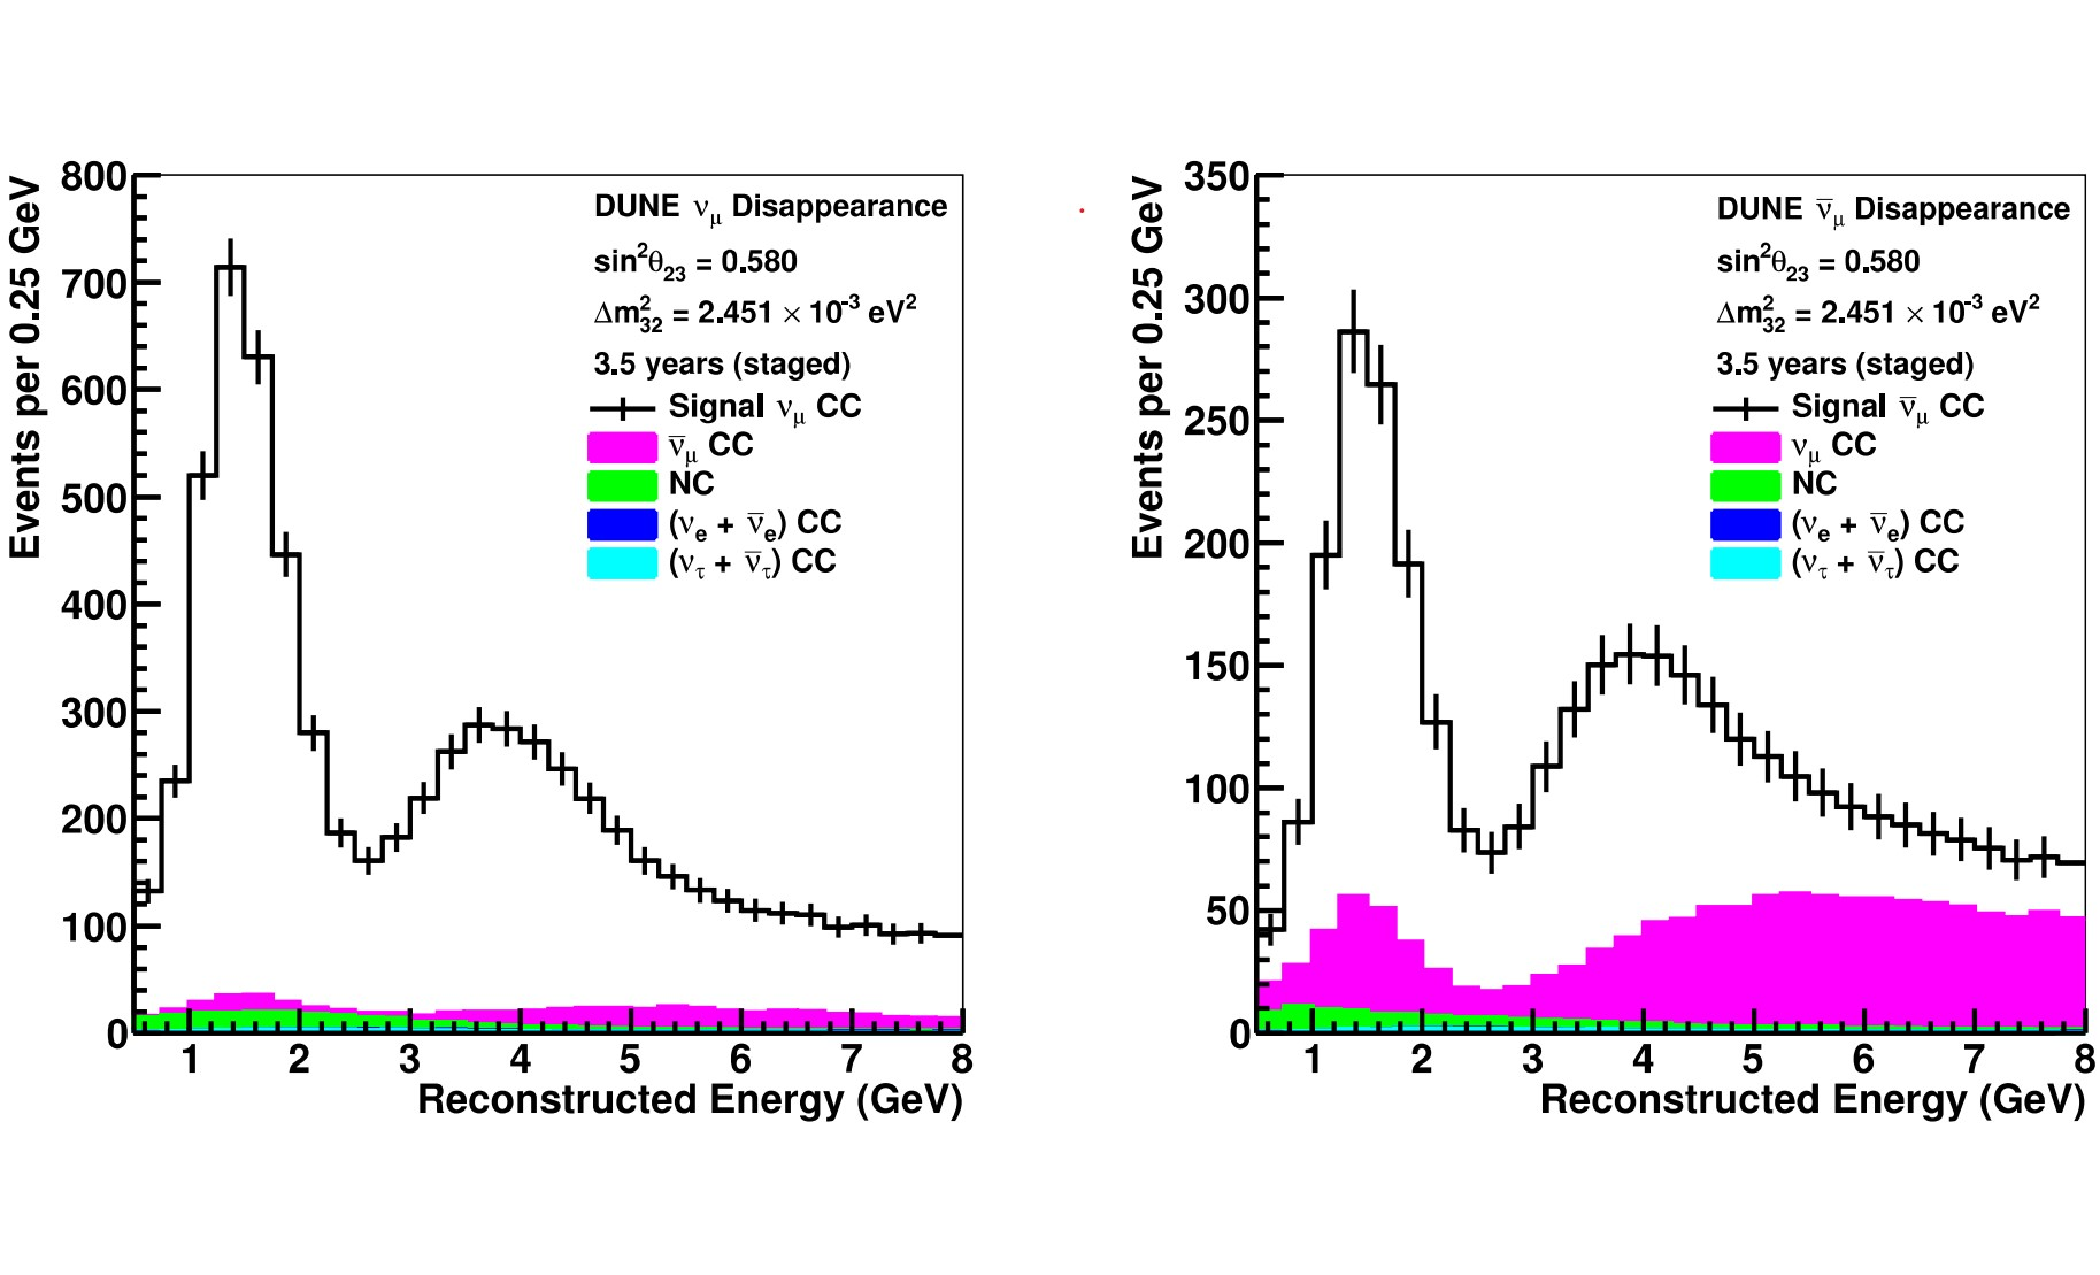
\includegraphics[width=\textwidth]{images/tdr_muon_reconstruction_tdrv2.pdf}
\caption{Figure is taken directly from the DUNE-FD TDR~\citep{DUNE_FD_TDRv2_2020}.
Images show the $\nu_{\mu}$ and $\bar{\nu_{\mu}}$ appearance spectra respectively.
}
\end{figure}~\label{fig:muon_interaction}

\printbibliography[heading=bibintoc]
% \printbibliography

%% appendix work on SVSC?
\appendix

% \chapter{SVSC OS1}
% \label{chap:OS1}
% the work in this subsection details the work and results of \cite{svsc_os1_aline_2021}. 

% \chapter{SVSC OS2}
% \label{chap:OS2}
% The section lists the work detailed in \citep{svsc_os2_Keefe_2022}.

\chapter{Neutrino Interaction Integral Data}~\label{app:integral_data}
\begin{longtable}{|l|l|l|l|l|l|}
			\hline
			lepton Pdg & Horn Current Direction & Z-Pos & Theta & 95\% Capture & 99\% Capture \\
			\hline
			12 & forward & 10 & 0 & 262 & 398 \\
			\hline
			12 & forward & 80 & 0 & 270 & 402 \\
			\hline
			12 & forward & 180 & 0 & 262 & 402 \\
			\hline
			12 & forward & 280 & 0 & 254 & 378 \\
			\hline
			12 & forward & 350 & 0 & 242 & 378 \\
			\hline
			12 & forward & 10 & 2 & 266 & 390 \\
			\hline
			12 & forward & 80 & 2 & 270 & 422 \\
			\hline
			12 & forward & 180 & 2 & 270 & 414 \\
			\hline
			12 & forward & 280 & 2 & 258 & 378 \\
			\hline
			12 & forward & 350 & 2 & 238 & 398 \\
			\hline
			12 & forward & 10 & -2 & 266 & 426 \\
			\hline
			12 & forward & 80 & -2 & 266 & 426 \\
			\hline
			12 & forward & 180 & -2 & 266 & 410 \\
			\hline
			12 & forward & 280 & -2 & 258 & 398 \\
			\hline
			12 & forward & 350 & -2 & 246 & 366 \\
			\hline
			12 & forward & 10 & 90 & 946 & 1526 \\
			\hline
			12 & forward & 80 & 90 & 950 & 1554 \\
			\hline
			12 & forward & 180 & 90 & 922 & 1638 \\
			\hline
			12 & forward & 280 & 90 & 798 & 1426 \\
			\hline
			12 & forward & 350 & 90 & 238 & 326 \\
			\hline
			12 & forward & 10 & -90 & 274 & 390 \\
			\hline
			12 & forward & 80 & -90 & 874 & 1570 \\
			\hline
			12 & forward & 180 & -90 & 954 & 1670 \\
			\hline
			12 & forward & 280 & -90 & 918 & 1586 \\
			\hline
			12 & forward & 350 & -90 & 906 & 1666 \\
			\hline
			-12 & forward & 10 & 0 & 238 & 362 \\
			\hline
			-12 & forward & 80 & 0 & 246 & 370 \\
			\hline
			-12 & forward & 180 & 0 & 234 & 358 \\
			\hline
			-12 & forward & 280 & 0 & 230 & 370 \\
			\hline
			-12 & forward & 350 & 0 & 214 & 334 \\
			\hline
			-12 & forward & 10 & 2 & 230 & 358 \\
			\hline
			-12 & forward & 80 & 2 & 238 & 382 \\
			\hline
			-12 & forward & 180 & 2 & 234 & 350 \\
			\hline
			-12 & forward & 280 & 2 & 226 & 350 \\
			\hline
			-12 & forward & 350 & 2 & 214 & 330 \\
			\hline
			-12 & forward & 10 & -2 & 234 & 382 \\
			\hline
			-12 & forward & 80 & -2 & 238 & 358 \\
			\hline
			-12 & forward & 180 & -2 & 238 & 358 \\
			\hline
			-12 & forward & 280 & -2 & 226 & 362 \\
			\hline
			-12 & forward & 350 & -2 & 214 & 334 \\
			\hline
			-12 & forward & 10 & 90 & 710 & 1378 \\
			\hline
			-12 & forward & 80 & 90 & 686 & 1274 \\
			\hline
			-12 & forward & 180 & 90 & 666 & 1350 \\
			\hline
			-12 & forward & 280 & 90 & 582 & 1250 \\
			\hline
			-12 & forward & 350 & 90 & 206 & 306 \\
			\hline
			-12 & forward & 10 & -90 & 238 & 354 \\
			\hline
			-12 & forward & 80 & -90 & 634 & 1358 \\
			\hline
			-12 & forward & 180 & -90 & 670 & 1358 \\
			\hline
			-12 & forward & 280 & -90 & 702 & 1454 \\
			\hline
			-12 & forward & 350 & -90 & 666 & 1354 \\
			\hline
			-12 & reverse & 10 & 0 & 222 & 342 \\
			\hline
			-12 & reverse & 80 & 0 & 226 & 334 \\
			\hline
			-12 & reverse & 180 & 0 & 226 & 326 \\
			\hline
			-12 & reverse & 280 & 0 & 218 & 322 \\
			\hline
			-12 & reverse & 350 & 0 & 202 & 306 \\
			\hline
			-12 & reverse & 10 & 2 & 226 & 322 \\
			\hline
			-12 & reverse & 80 & 2 & 222 & 330 \\
			\hline
			-12 & reverse & 180 & 2 & 222 & 326 \\
			\hline
			-12 & reverse & 280 & 2 & 214 & 318 \\
			\hline
			-12 & reverse & 350 & 2 & 198 & 290 \\
			\hline
			-12 & reverse & 10 & -2 & 218 & 326 \\
			\hline
			-12 & reverse & 80 & -2 & 226 & 342 \\
			\hline
			-12 & reverse & 180 & -2 & 218 & 318 \\
			\hline
			-12 & reverse & 280 & -2 & 214 & 322 \\
			\hline
			-12 & reverse & 350 & -2 & 202 & 306 \\
			\hline
			-12 & reverse & 10 & 90 & 710 & 1374 \\
			\hline
			-12 & reverse & 80 & 90 & 674 & 1378 \\
			\hline
			-12 & reverse & 180 & 90 & 642 & 1434 \\
			\hline
			-12 & reverse & 280 & 90 & 578 & 1266 \\
			\hline
			-12 & reverse & 350 & 90 & 194 & 286 \\
			\hline
			-12 & reverse & 10 & -90 & 230 & 330 \\
			\hline
			-12 & reverse & 80 & -90 & 590 & 1314 \\
			\hline
			-12 & reverse & 180 & -90 & 622 & 1334 \\
			\hline
			-12 & reverse & 280 & -90 & 674 & 1398 \\
			\hline
			-12 & reverse & 350 & -90 & 638 & 1310 \\
			\hline
			14 & forward & 10 & 0 & 258 & 370 \\
			\hline
			14 & forward & 80 & 0 & 258 & 386 \\
			\hline
			14 & forward & 180 & 0 & 254 & 366 \\
			\hline
			14 & forward & 280 & 0 & 246 & 358 \\
			\hline
			14 & forward & 350 & 0 & 238 & 338 \\
			\hline
			14 & forward & 10 & 2 & 258 & 382 \\
			\hline
			14 & forward & 80 & 2 & 258 & 398 \\
			\hline
			14 & forward & 180 & 2 & 258 & 394 \\
			\hline
			14 & forward & 280 & 2 & 246 & 334 \\
			\hline
			14 & forward & 350 & 2 & 226 & 338 \\
			\hline
			14 & forward & 10 & -2 & 254 & 378 \\
			\hline
			14 & forward & 80 & -2 & 262 & 386 \\
			\hline
			14 & forward & 180 & -2 & 254 & 354 \\
			\hline
			14 & forward & 280 & -2 & 238 & 346 \\
			\hline
			14 & forward & 350 & -2 & 230 & 326 \\
			\hline
			14 & forward & 10 & 90 & 786 & 1534 \\
			\hline
			14 & forward & 80 & 90 & 798 & 1470 \\
			\hline
			14 & forward & 180 & 90 & 754 & 1454 \\
			\hline
			14 & forward & 280 & 90 & 682 & 1338 \\
			\hline
			14 & forward & 350 & 90 & 234 & 322 \\
			\hline
			14 & forward & 10 & -90 & 258 & 382 \\
			\hline
			14 & forward & 80 & -90 & 726 & 1494 \\
			\hline
			14 & forward & 180 & -90 & 778 & 1490 \\
			\hline
			14 & forward & 280 & -90 & 766 & 1366 \\
			\hline
			14 & forward & 350 & -90 & 786 & 1482 \\
			\hline
			14 & reverse & 10 & 0 & 270 & 382 \\
			\hline
			14 & reverse & 80 & 0 & 278 & 406 \\
			\hline
			14 & reverse & 180 & 0 & 266 & 394 \\
			\hline
			14 & reverse & 280 & 0 & 258 & 378 \\
			\hline
			14 & reverse & 350 & 0 & 242 & 366 \\
			\hline
			14 & reverse & 10 & 2 & 274 & 402 \\
			\hline
			14 & reverse & 80 & 2 & 282 & 390 \\
			\hline
			14 & reverse & 180 & 2 & 266 & 398 \\
			\hline
			14 & reverse & 280 & 2 & 262 & 374 \\
			\hline
			14 & reverse & 350 & 2 & 242 & 374 \\
			\hline
			14 & reverse & 10 & -2 & 262 & 406 \\
			\hline
			14 & reverse & 80 & -2 & 274 & 418 \\
			\hline
			14 & reverse & 180 & -2 & 262 & 378 \\
			\hline
			14 & reverse & 280 & -2 & 258 & 394 \\
			\hline
			14 & reverse & 350 & -2 & 238 & 354 \\
			\hline
			14 & reverse & 10 & 90 & 942 & 1570 \\
			\hline
			14 & reverse & 80 & 90 & 898 & 1618 \\
			\hline
			14 & reverse & 180 & 90 & 842 & 1550 \\
			\hline
			14 & reverse & 280 & 90 & 822 & 1522 \\
			\hline
			14 & reverse & 350 & 90 & 234 & 334 \\
			\hline
			14 & reverse & 10 & -90 & 270 & 406 \\
			\hline
			14 & reverse & 80 & -90 & 838 & 1526 \\
			\hline
			14 & reverse & 180 & -90 & 898 & 1610 \\
			\hline
			14 & reverse & 280 & -90 & 914 & 1562 \\
			\hline
			14 & reverse & 350 & -90 & 894 & 1642 \\
			\hline
			-14 & forward & 10 & 0 & 222 & 326 \\
			\hline
			-14 & forward & 80 & 0 & 226 & 334 \\
			\hline
			-14 & forward & 180 & 0 & 214 & 322 \\
			\hline
			-14 & forward & 280 & 0 & 210 & 314 \\
			\hline
			-14 & forward & 350 & 0 & 194 & 302 \\
			\hline
			-14 & forward & 10 & 2 & 218 & 342 \\
			\hline
			-14 & forward & 80 & 2 & 222 & 330 \\
			\hline
			-14 & forward & 180 & 2 & 214 & 322 \\
			\hline
			-14 & forward & 280 & 2 & 210 & 314 \\
			\hline
			-14 & forward & 350 & 2 & 198 & 290 \\
			\hline
			-14 & forward & 10 & -2 & 218 & 322 \\
			\hline
			-14 & forward & 80 & -2 & 222 & 322 \\
			\hline
			-14 & forward & 180 & -2 & 214 & 310 \\
			\hline
			-14 & forward & 280 & -2 & 206 & 314 \\
			\hline
			-14 & forward & 350 & -2 & 202 & 298 \\
			\hline
			-14 & forward & 10 & 90 & 578 & 1274 \\
			\hline
			-14 & forward & 80 & 90 & 578 & 1254 \\
			\hline
			-14 & forward & 180 & 90 & 522 & 1186 \\
			\hline
			-14 & forward & 280 & 90 & 490 & 1046 \\
			\hline
			-14 & forward & 350 & 90 & 182 & 270 \\
			\hline
			-14 & forward & 10 & -90 & 218 & 314 \\
			\hline
			-14 & forward & 80 & -90 & 546 & 1214 \\
			\hline
			-14 & forward & 180 & -90 & 570 & 1150 \\
			\hline
			-14 & forward & 280 & -90 & 538 & 1190 \\
			\hline
			-14 & forward & 350 & -90 & 550 & 1238 \\
			\hline
			-14 & reverse & 10 & 0 & 218 & 338 \\
			\hline
			-14 & reverse & 80 & 0 & 218 & 326 \\
			\hline
			-14 & reverse & 180 & 0 & 210 & 318 \\
			\hline
			-14 & reverse & 280 & 0 & 206 & 306 \\
			\hline
			-14 & reverse & 350 & 0 & 194 & 294 \\
			\hline
			-14 & reverse & 10 & 2 & 210 & 318 \\
			\hline
			-14 & reverse & 80 & 2 & 210 & 338 \\
			\hline
			-14 & reverse & 180 & 2 & 218 & 326 \\
			\hline
			-14 & reverse & 280 & 2 & 206 & 302 \\
			\hline
			-14 & reverse & 350 & 2 & 194 & 278 \\
			\hline
			-14 & reverse & 10 & -2 & 218 & 310 \\
			\hline
			-14 & reverse & 80 & -2 & 218 & 334 \\
			\hline
			-14 & reverse & 180 & -2 & 214 & 314 \\
			\hline
			-14 & reverse & 280 & -2 & 206 & 306 \\
			\hline
			-14 & reverse & 350 & -2 & 194 & 290 \\
			\hline
			-14 & reverse & 10 & 90 & 514 & 1098 \\
			\hline
			-14 & reverse & 80 & 90 & 486 & 1082 \\
			\hline
			-14 & reverse & 180 & 90 & 498 & 1102 \\
			\hline
			-14 & reverse & 280 & 90 & 446 & 1030 \\
			\hline
			-14 & reverse & 350 & 90 & 174 & 266 \\
			\hline
			-14 & reverse & 10 & -90 & 218 & 326 \\
			\hline
			-14 & reverse & 80 & -90 & 486 & 1014 \\
			\hline
			-14 & reverse & 180 & -90 & 494 & 1110 \\
			\hline
			-14 & reverse & 280 & -90 & 494 & 1122 \\
			\hline
			-14 & reverse & 350 & -90 & 506 & 1118 \\
			\hline
			12 & reverse & 10 & 0 & 286 & 426 \\
			\hline
			12 & reverse & 80 & 0 & 290 & 426 \\
			\hline
			12 & reverse & 180 & 0 & 286 & 422 \\
			\hline
			12 & reverse & 280 & 0 & 278 & 426 \\
			\hline
			12 & reverse & 350 & 0 & 262 & 410 \\
			\hline
			12 & reverse & 10 & 2 & 282 & 422 \\
			\hline
			12 & reverse & 80 & 2 & 286 & 430 \\
			\hline
			12 & reverse & 180 & 2 & 286 & 454 \\
			\hline
			12 & reverse & 280 & 2 & 278 & 426 \\
			\hline
			12 & reverse & 350 & 2 & 250 & 422 \\
			\hline
			12 & reverse & 10 & -2 & 270 & 434 \\
			\hline
			12 & reverse & 80 & -2 & 294 & 446 \\
			\hline
			12 & reverse & 180 & -2 & 286 & 446 \\
			\hline
			12 & reverse & 280 & -2 & 274 & 426 \\
			\hline
			12 & reverse & 350 & -2 & 258 & 382 \\
			\hline
			12 & reverse & 10 & 90 & 1126 & 1774 \\
			\hline
			12 & reverse & 80 & 90 & 1098 & 1630 \\
			\hline
			12 & reverse & 180 & 90 & 1014 & 1694 \\
			\hline
			12 & reverse & 280 & 90 & 910 & 1498 \\
			\hline
			12 & reverse & 350 & 90 & 246 & 362 \\
			\hline
			12 & reverse & 10 & -90 & 286 & 406 \\
			\hline
			12 & reverse & 80 & -90 & 970 & 1658 \\
			\hline
			12 & reverse & 180 & -90 & 1114 & 1686 \\
			\hline
			12 & reverse & 280 & -90 & 1022 & 1770 \\
			\hline
			12 & reverse & 350 & -90 & 1014 & 1622 \\
			\hline
	\caption{APA Integral Data.
	Integrals are performed on histograms of bin widths of two.
	}
	\label{tab:apa_sum}
\end{longtable}

\printindex

\end{document}
